% REVISION v56: 2026-07-31
% Reviewer/annotation integration pass:
% clarified the material base and calculus-relative carrier; integrated
% context derivatives, Green series, and CK resource use; sharpened the
% independence, harmony, base-extension, and future-work boundaries.
\documentclass[10pt,a4paper]{article}

\usepackage{cmap}
\usepackage[T1]{fontenc}
\usepackage{lmodern}
\usepackage{microtype}
\usepackage{amsmath,amssymb,amsthm,mathtools}
\usepackage{enumitem}
\usepackage{booktabs,array,longtable}
\usepackage{tikz}
\usepackage{graphicx}
\usepackage{float}
\usepackage[margin=1in]{geometry}
\usepackage[hidelinks]{hyperref}

\setlength{\emergencystretch}{3em}
\setlist{nosep}
\allowdisplaybreaks

\theoremstyle{plain}
\newtheorem{theorem}{Theorem}[section]
\newtheorem{proposition}[theorem]{Proposition}
\newtheorem{lemma}[theorem]{Lemma}
\newtheorem{corollary}[theorem]{Corollary}
\theoremstyle{definition}
\newtheorem{definition}[theorem]{Definition}
\newtheorem{example}[theorem]{Example}
\theoremstyle{remark}
\newtheorem{remark}[theorem]{Remark}

\newcommand{\Base}{\mathcal B}
\newcommand{\Rules}{\mathcal R}
\newcommand{\Lang}{\mathcal L}
\newcommand{\Trees}{\mathsf T}
\newcommand{\Forests}{\mathsf F}
\newcommand{\HCK}{H_{\mathrm{CK}}}
\newcommand{\Hlic}{H_{\Base,\Rules}}
\newcommand{\DeltaCK}{\Delta_{\mathrm{CK}}}
\newcommand{\epsCK}{\varepsilon_{\mathrm{CK}}}
\newcommand{\ms}{\mathrel{\vdash}}
\newcommand{\rootseq}{\operatorname{bd}}
\newcommand{\Root}{\operatorname{Root}}
\newcommand{\BRoot}{\operatorname{BRoot}}
\newcommand{\FlatRoot}{\operatorname{flat}}
\newcommand{\HSeq}{\mathsf{HSeq}}
\newcommand{\fjoin}{\mathbin{\sqcup}}
\newcommand{\one}{\mathbf 1}
\newcommand{\Fill}{\operatorname{Fill}}
\newcommand{\Req}{\operatorname{req}}
\newcommand{\Punc}{\operatorname{Punc}}
\newcommand{\Comp}{\operatorname{Comp}}
\newcommand{\Tel}{\operatorname{Tel}}
\newcommand{\br}{\operatorname{br}}
\newcommand{\Ctx}{\mathsf{Ctx}}
\newcommand{\Prf}{\mathsf{Prf}}
\newcommand{\OpenPrf}{\mathsf{OpenPrf}}
\newcommand{\parr}{\mathbin{\rotatebox[origin=c]{180}{\&}}}
\newcommand{\eqtag}{\refstepcounter{equation}\tag{\theequation}}
\newcolumntype{L}[1]{>{\raggedright\arraybackslash}p{#1}}

\title{The Connes--Kreimer Hopf Algebra and Hypersequent Proof Trees}
\author{}
\date{}

\begin{document}
\maketitle

\begin{abstract}
We ask what the Connes--Kreimer decomposition of hypersequent proof trees
contributes to proof-theoretic semantics.  Cutting an ancestry antichain
detaches subproofs and leaves the typed context which uses them; filling the
punctures reconstructs or varies the proof.  A typed Fa\`a di Bruno law relates
retrospective cutting to prospective context composition.  Two positive
interpretations result.  Backward-refinement histories modulo exchange of
independent steps are precisely proof contexts, CK cuts are the frontiers of
their presentation-causality ideals, and convolution powers of the all-ones
and degree-one functionals count staged decompositions and complete
construction schedules, respectively.
Moreover, proof operations uniform under typed proof substitution are
represented by open contexts.  Filling repeated formal inputs by fresh probes
and evaluating the CK coproduct by two characters gives the resource polynomial
\(\prod_i(1+z_i)^{\nu_i}\); it detects linear, affine, relevant, erasing, and
independently copying uses of supplied proofs.  These results use cut support
and multiplicity rather than rule names.  The same construction then tests
proof identity.  Local rule-interface symmetries give CK-stable quotients, but
neither a harmonious tensor reduction nor a standard permutation between
sequentialisations of one MLL proof net can belong to any CK-stable proof
congruence on this tree carrier.  Component traces finally distinguish
Communication from ordinary assembly and separate consequence-equivalent
calculi with different direct Gentzen-Cut-free proof operations.
\end{abstract}

\section*{Introduction}

Many central ideas in proof theory and proof-theoretic semantics---including
harmony, polarity, proof-theoretic validity, and proof identity---have been
articulated through the analysis of introduction and use rules for logical
vocabulary
\cite{prawitz1965,dummett1991,schroederheister2015,
pistonetranchini2024}.  This paper studies a complementary aspect of proof
structure.  Once a sequent or hypersequent calculus and a material base are
fixed, which families of subproof occurrences can be detached
simultaneously, what typed residual context records their use, and which
such decompositions survive when the proof is transformed or identified
with another?  Here a \emph{material ground} is a tagged terminal proof
object supplied by the base for an accepted primitive-boundary inference,
rather than by a logical or structural rule.  The base need not be monotone
or closed under Weakening, Contraction, or composition.

The Connes--Kreimer admissible-cut construction gives an algebraic treatment
of this question.  We read a derivation as a rooted tree whose vertices are
concrete rule occurrences and whose indexed child edges identify their
premise positions.  A CK-admissible cut selects an antichain of subproofs
in the premise-ancestry order, so none contains another.  Removing them
leaves the root conclusion together with the
surrounding derivation, punctured at the premise positions formerly occupied
by those subproofs.

\begin{figure}[H]
\centering
\[
\begin{gathered}
t=
\underbrace{
 \frac{\pi:G_1\qquad \sigma:G_2}{G}\;a
}_{a(\pi,\sigma)}
\quad\xmapsto{\ \text{cut both premise edges}\ }\quad
\underbrace{\pi\fjoin\sigma}_{P^c(t)}
\ \otimes\
\underbrace{
 \frac{\Box_1:G_1\qquad\Box_2:G_2}{G}\;a
}_{R^c(t)},\\[4pt]
R^c(t)[\Box_1:=\pi,\Box_2:=\sigma]=t,\qquad
R^c(t)[\Box_1:=\pi',\Box_2:=\sigma']
\ \text{is defined when }\rootseq(\pi')=G_1,\ \rootseq(\sigma')=G_2 .
\end{gathered}
\]
\caption{A CK cut and its proof-theoretic reading.  The boundaries
\(G_1,G_2,G\) may be hypersequents.  Reinstating the selected proofs gives
the distinguished reconstruction of \(t\); inserting other complete proofs
of \(G_1,G_2\) is filling, while inserting punctured contexts is context
composition.}
\label{fig:intro-ck-cut}
\end{figure}

The construction has retrospective and prospective readings.  Retrospectively,
the cut records which subproofs a completed proof used and the rule context
in which they occurred.  Prospectively, the punctured context may be
completed by any proofs of the required premises available in the calculus;
the proofs originally removed are one possible filling, not privileged
contents of the punctures.  Linearising all admissible cuts gives the CK
coproduct, while multiplication forms the commutative forest of separate
proof trees.  The roots of such a forest can be flattened to one
hypersequent boundary, but multiplication is neither an external rule nor a
connected proof of that hypersequent.  Successive cuts record nested stages
of proof construction.

This factorisation has a causal reading, but a deliberately proof-specific
one.  Starting from an open conclusion, a proof context may be built by
refining currently open premise positions.  Refinements at independent
positions commute, while a premise rule cannot be introduced before the rule
whose premise it fills.  The CK coproduct sees the same dependency in reverse:
its terms are causal frontiers between a detached proof region and the context
which uses it, and its convolution powers count staged decompositions.  A
second reading concerns hypothetical proof use.  Once distinct open
occurrences are allowed to name the same formal input, the coproduct records
every independently detachable subfamily of the resulting proof copies.  The
history quotient uses strict interchange of independent context refinements;
its CK incidence refinement and the resource statements use coproduct support
and multiplicity, not classifications extracted from logical rule names.

Two small calculations preview the positive and negative payoffs.  If a
represented operation uses one formal proof twice,
\(R(x)=a(x,x)\), then the two singleton probe cuts and their simultaneous
cut give
\[
                    \mathsf Q_R(z)=1+2z+z^2;
\]
the coefficient \(2\) counts cut addresses rather than reading a
Contraction tag.  Conversely, the two familiar sequentialisations of one
MLL proof net have the same inputs and conclusion but expose different
intermediate proof boundaries.  The resource profile therefore agrees
while raw CK factorisation separates them.

Hypersequents make the distinction between these operations particularly
important.  A connected proof of a displayed hypersequent is not the same
proof object as a forest of independent proofs whose conclusions flatten
to that hypersequent.  Moreover, external structural rules may move, divide,
or recombine component occurrences in ways which scalar tree data do not
detect.  We therefore retain at each rule vertex the component-incidence
data recording which indexed premise-component occurrences contribute to
which indexed conclusion components, and compose these relations along the
punctured contexts exposed by CK cuts.

The logical and structural regime is supplied by the underlying calculus.
Its logical rules, structural rules, normalisation conversions, and proposed
proof equations are supplied by that calculus and justified on
proof-theoretic grounds independently of the CK structure.  The
Hopf-algebraic analysis
asks what those transformations preserve: their input proofs, their
component action, and their decomposition into detached evidence and a
surrounding proof context.  This separates the proof-theoretic justification
of an equation from the further question whether CK factorisation is
well-defined on the resulting proof classes.

Section~\ref{sec:interfaces} constructs the proof-tree carrier, punctured
derivations, and filling, and relates the one-hole case to the
differential/zipper account of datatype contexts developed by McBride and
Abbott et al.~\cite{mcbride2001,abbott2003derivatives}.
Section~\ref{sec:factorisation} linearises CK cuts,
proves a typed Fa\`a di Bruno identity for context composition, recovers
premise ancestry from iterated cuts, identifies refinement traces and their
Hopf-convolution counts, and studies changes of material base.
Section~\ref{sec:identity} adds component traces and the coideal criterion
for proof equations, proves CK stability for local interface symmetries, and
contrasts them with an MLL proof-net permutation.  Section~\ref{sec:harmony} separates factorisations
internal to fixed input proofs from those contributed by a surrounding rule
context, represents substitution-uniform hypothetical operations, extracts
their CK resource-use polynomials, and applies the relative construction to
local Gentzen-Cut reduction and harmony.
Section~\ref{sec:communication} gives the specifically hypersequent
application to Communication and analytic proof structure.

The paper can also be read payoff first.  Readers primarily interested in
the positive semantics may begin with the causal-schedule theorem in
Theorem~\ref{thm:causal-ck-semantics} and the resource-use theorem in
Theorem~\ref{thm:ck-resource-polynomial}.  Readers primarily interested in
harmony and proof identity may begin with the positive local-symmetry quotient
in Proposition~\ref{prop:local-symmetry-ck-stable}, the proof-net obstruction in
Example~\ref{ex:mll-permutation-obstruction}, the tensor and \(\mathbin{\mathrm{tonk}}\)
comparison in Proposition~\ref{prop:positive-tensor-harmony} and
Example~\ref{ex:tonk-disharmony}, and the Communication application in
Section~\ref{sec:communication}.  They can then return to
Sections~\ref{sec:interfaces}--\ref{sec:identity} for the constructions
supporting those tests.  The dictionary below gives the intended
proof-theoretic reading of the imported algebraic vocabulary; the formal
definitions remain in the body of the paper, and the final notation index
records symbols by section.

\section*{Reader's dictionary}

The entries in this table are orientation rather than substitute
definitions.  In particular, algebraic inversion is not proof reduction,
and a quotient becomes a semantics of proof identity only after the chosen
proof calculus has supplied and proof-theoretically justified the equations
being imposed.

\begingroup
\small
\begin{longtable}{@{}L{4.0cm}L{10.7cm}@{}}
\toprule
algebraic or combinatorial term & proof-theoretic reading in this paper\\
\midrule
\endfirsthead
\toprule
algebraic or combinatorial term & proof-theoretic reading in this paper\\
\midrule
\endhead
\midrule
\multicolumn{2}{r}{\small continued on next page}\\
\endfoot
\bottomrule
\endlastfoot
forest, basis symbol \([F]\), product
& A finite multiset of complete or punctured derivation trees.  \([F]\) is
  its basis symbol; formal sums combine outcomes with coefficients, and
  multiplication juxtaposes independent proof blocks.  Flattening their
  root boundaries displays a hypersequent profile, not a connected proof of
  that hypersequent.\\
CK cut and coproduct \(\DeltaCK\)
& A cut selects an ancestry antichain of subderivations.  The coproduct is the
  formal sum of all pairs consisting of the detached forest and the
  punctured remainder.\\
ancestry incidence map, order character
& Forgetting proof decorations sends the CK coproduct to the incidence
  coproduct of causal ideals.  Convolution powers count causal layerings;
  restricting every layer to one vertex counts complete construction
  schedules.\\
counit \(\epsCK\)
& The bookkeeping map which returns \(1\) on the empty forest and \(0\) on
  every nonempty forest; it is not a truth valuation.\\
puncture, filling fibre, corolla, telescope, zipper
& Respectively: an open premise position; all compatible tuples of complete
  proofs which can fill the open positions; one rule occurrence with every
  premise open; the ordered open positions together with their boundary
  requirements; and the factorisation of
  a marked subproof into that subproof and its one-hole context.  A nullary
  corolla has no open premises and is already a complete proof.\\
polynomial grammar and derivative
& A sum over possible rule constructors, with a product over their premise
  slots.  Its formal derivative marks one selected proof-input occurrence
  and retains the context surrounding it.\\
operad and context insertion
& The operad is the typed associative composition of proof contexts with
  identities; it is a compact name for the insertion operations already
  present in the proof grammar.\\
Green series and Fa\`a di Bruno identity
& A Green series is the formal inventory of all contexts of one interface.
  The identity collects every way to read a composite context as inner
  proof contexts inserted into an outer context.\\
CK resource polynomial \(\mathsf Q_R\)
& Fill every occurrence of a formal proof input by a fresh probe, take the
  CK coproduct, and evaluate its two factors by probe and all-ones
  characters.  Integrally, coefficients count simultaneous probe selections
  (with the whole-tree endpoint handling a nodeless identity) and hence
  independently copied, erased, or single uses of supplied proofs.\\
coaction, comodule, comodule map
& A coaction is a coproduct-like observation which keeps the root-containing
  remainder---or the retained tuple of pointed inputs---in a distinguished
  right-hand factor.  A comodule is a space carrying such an observation; a comodule map
  preserves it.\\
coideal, Hopf ideal, quotient
& Together with counit compatibility, the coideal condition is precisely
  what lets a coproduct be computed on equivalence classes rather than
  representatives.  A Hopf ideal is an algebra ideal which also satisfies
  this coideal condition, has zero counit, and is stable under the antipode;
  its quotient retains the Hopf structure.\\
local rule-interface symmetry
& A presentation change confined to one rule occurrence: its boundary is
  fixed, while component action and formula incidences are transported by
  chosen occurrence reindexings; genuinely
  symmetric premise slots may be permuted or a local evidence tag forgotten.
  Such a change preserves ancestry and transports CK cuts one-for-one.\\
context-relative residue \(\Omega_s\); protected replacement residue
\(\operatorname{Res}^{\mathsf{Prot}}\)
& The first subtracts cuts wholly internal to every designated input and
  retains cuts entering the fixed outer context.  The second compares two
  maps after subtracting only the protected inputs' decompositions, so
  changes involving unprotected inputs remain.  Its projection is complete
  for the displayed comparison ideal; full contextual closure is tested
  separately.\\
convolution and antipode
& Convolution combines two maps by first decomposing an input, applying one
  map to each factor, and multiplying the results.  The antipode supplies
  the recursive formal cancellation required for a convolution inverse; it
  does not invert proofs or reduce Gentzen Cuts.\\
\end{longtable}
\endgroup

\section{Material inference and rooted proof trees}
\label{sec:interfaces}

\subsection{Boundaries, rule vertices, and component focus}

Fix a finitary formula language \(\Lang\) with a chosen primitive formula
sublanguage \(\Lang_{\mathrm{pr}}\), often the atomic formulae.  The
primitive material objects below are not bare formulae: they are sequents
or hypersequents all of whose formula occurrences lie in
\(\Lang_{\mathrm{pr}}\).  Write \(\mathsf M_f(X)\) for the finite
multisets over \(X\).  Throughout, we treat formula contexts as finite
multisets of formulae and hypersequents as finite nonempty multisets of
sequents.  A sequent is a pair \(\Gamma\ms\Delta\).  A \emph{proof-boundary
hypersequent} is a finite nonempty multiset
\[
                 G=S_1\mid\cdots\mid S_n .
\]
Write \(\HSeq\) for their set, identifying a sequent with its singleton
hypersequent.  If \(G=(S_j)_{j\in I_G}\), then
\(\Comp(G)=I_G\) is its finite set of component \emph{occurrences}.
This indexing matters when two displayed components are equal: they remain
two occurrences.  A coherent reindexing is a bijection between equal
multiset occurrences which preserves the displayed formula and component
incidences.

Thus internal Exchange is already absorbed by equality of formula contexts,
and external Exchange by coherent
reindexing of component occurrences.  Neither convention identifies the
first and second premise slots of a binary rule.  Nor does it add
Weakening or Contraction; any such rule used by a proof is an explicit
rule occurrence.  Empty boundary hypersequents are excluded, while
\(\one\) will denote the empty proof forest.

A familiar component-local instance illustrates the data retained at a
vertex:
\[
 \frac{\mathcal G\mid\Gamma,A\ms B}
      {\mathcal G\mid\Gamma\ms A\to B}\;(\to R).
\eqtag\label{eq:component-local-example}
\]
The premise and conclusion are whole hypersequents.  The displayed
\(\to R\)-occurrence acts on one component and carries every companion
component in \(\mathcal G\) unchanged.  By an \emph{external rule} here we
mean one whose principal action changes or relates the hypersequent
component structure, rather than a sequent rule acting within one component
while carrying every companion component unchanged.  Communication will
provide the main example in Section~\ref{sec:communication}.

Write \(\HSeq_{\mathrm{pr}}\) for hypersequents all of whose formulae lie
in the primitive fragment, and fix a stock \(\Rules\) of rule symbols,
each with finite proof-rule arity.

The definitions permit arbitrary finite rule arity, although the displayed
sequent and hypersequent rules are nullary, unary, or binary.  Arity here
counts immediate proof premises, not hypersequent breadth or the number of
punctures accumulated through a proof.

\begin{definition}[Concrete rule occurrence]
\label{def:concrete-occurrence}
A \emph{concrete rule occurrence} is a finitary constructor with indexed
premise slots
\[
 a=(\rho,\theta):
   (G^a_1,\ldots,G^a_{n(a)})\longrightarrow G^a ,
\eqtag\label{eq:equipped-rule}
\]
where \(\rho\) is the rule tag and \(\theta\) is its fully instantiated
formula and context data.  The premises are ordered: for a binary rule they
are its literal left and right proof premises.  Write
\(\operatorname{in}_i(a)=G^a_i\) and
\(\operatorname{out}(a)=G^a\).
\end{definition}

The instance data \(\theta\) determine a component relation
\[
 \kappa_a\subseteq
 \left(\bigsqcup_{i=1}^{n(a)}
    \{i\}\times\Comp(G^a_i)\right)
 \times\Comp(G^a).
\eqtag\label{eq:component-relation}
\]
Read \(((i,c),d)\in\kappa_a\) as saying that component occurrence \(c\)
of premise \(i\) contributes tracked occurrence data to conclusion
component \(d\).
For a logical or internal structural rule, \(\theta\) selects one active
component occurrence in each relevant premise and conclusion, together
with its active and principal formula occurrences.  The relation
\(\kappa_a\) includes the active action and the concrete bijections which
carry passive component occurrences unchanged; equal passive components
remain distinct occurrences.  For such an external rule, \(\theta\)
may select several active components and \(\kappa_a\) may be a general
finite relation.  Any formula-occurrence incidence, discharge, or pairing
used below is likewise read from the concrete instance.  If a material rule tag
does not determine such incidence, the required relation is included in
\(\theta\); it is not duplicated as extra decoration on every vertex.
The occurrence is \emph{primitive-boundary} when all \(G^a_i,G^a\) lie in
\(\HSeq_{\mathrm{pr}}\).

For example, if \(p,q,r\) are primitive formulae, a small material base
might contain two tagged grounds
\[
 b_{pq}:()\longrightarrow(p\ms q),
 \qquad
 b_{qr}:()\longrightarrow(q\ms r).
\eqtag\label{eq:small-material-base}
\]
These are proof objects for the displayed primitive inferences.  Their
presence alone supplies neither a proof of \(p\ms r\) nor any weakened or
contracted variant.

\begin{definition}[Material base and the equipped calculus]
\label{def:material-equipped}
A \emph{material base} \(\Base\) is a tagged set of primitive-boundary
material rule occurrences.  Constructor tags are part of their identity, so several
material inferences may have the same input--output profile.  Its nullary
subfamilies are
\[
 \Base^{(0)}_G
   =\{b\in\Base\mid n(b)=0,\ \operatorname{out}(b)=G\},
 \qquad
 \Base_0=\coprod_G\Base^{(0)}_G .
\]
Here \(\coprod\) is a disjoint union: it remembers the boundary \(G\) from
which an occurrence came even when two displayed sets happen to coincide.
No Weakening, Contraction, or Gentzen Cut occurrence is supplied merely by
this definition.  We distinguish material occurrences in \(\Base\),
logical initials, and the allowed instances of logical or structural
symbols in \(\Rules\) by disjoint tags.  A concrete occurrence
\emph{belongs to the equipped calculus} \((\Base,\Rules)\) when it is one
of these occurrences.  Thus
\(\Base_0\) supplies terminal material grounds, while positive-arity
members of \(\Base\) are primitive material inference operations in the
same recursive rule grammar.

A \emph{persistent material inclusion}
\(j:\Base\hookrightarrow\Base'\) identifies each old tagged material
occurrence with one having the same ordered proof-input arity, concrete
premise and conclusion boundaries, and component/formula-incidence data.
Thus \(\Base'\) may add material grounds or primitive material operations,
but it does not revise an old one.  This extends the material base within
the fixed language; it is not a formula-language extension.  After
identifying \(\Base\) with its image we write
\(\Base\subseteq\Base'\).
\end{definition}

An arbitrary primitive material support relation
\[
 B\subseteq\mathsf M_f(\Lang_{\mathrm{pr}})
          \times\mathsf M_f(\Lang_{\mathrm{pr}})
\]
can be represented discretely by assigning each accepted pair
\((\Gamma,\Delta)\in B\) one tagged nullary ground
\[
       \ulcorner\Gamma\ms\Delta\urcorner:
       ()\longrightarrow(\Gamma\ms\Delta).
\eqtag\label{eq:discrete-material-presentation}
\]
Here ``nullary'' refers only to proof-input arity: \(\Gamma\) remains part
of the sequent boundary.  This is a faithful discrete encoding of \(B\):
every accepted pair becomes a terminal proof generator, and no weakened,
contracted, or composed pair is added automatically.  Thus \(B\) determines
the terminal part of the proof-tree carrier and the available filling
fibres.  It may, for example, contain
\(\Gamma\ms\Delta\) while omitting
\(\Gamma,A\ms\Delta\); the former ground cannot fill the latter boundary.
A nonmonotone support relation therefore remains nonmonotone at the
material level, while any monotonic closure of the equipped calculus must
come from explicitly admitted material, structural, or logical rule
occurrences.  An inclusion of support relations gives a persistent
inclusion of their grounds.  Positive-arity material occurrences add
proof-relevant internal structure which the discrete presentation omits.

\subsection{Punctured derivations and filling fibres}

\begin{definition}[Proof tree and puncture]
\label{def:proof-tree}
A (possibly punctured) proof tree is written recursively as the
premise-slot-indexed term
\[
                    t=a(u_1,\ldots,u_{n(a)}),
\]
and we use \emph{term} for this constructor notation and \emph{tree} for
the rooted-tree presentation of the same object.  The root is decorated by
a concrete rule occurrence \(a\), and each
\(u_i\) is either a compatible rule-rooted proof term of boundary
\(\operatorname{in}_i(a)\) or a vacant premise symbol in that position.
Every vertex is an admitted concrete rule occurrence of the equipped
calculus; punctures are vacant positions, not vertices.  Thus the carrier
is calculus-relative: arbitrary decorated trees whose occurrences or
boundaries are incompatible with \((\Base,\Rules)\) are excluded.  Its root boundary is
\(\rootseq(t)=\operatorname{out}(a)\).  Vertices are addressed by finite
words of premise-slot indices; the root has address \(\epsilon\), and the
\(i\)-th child appends \(i\) to its parent's address.  Such a
\emph{premise-slot address} records successive choices of proof-premise
slots from the root.  It is a position in the proof tree, not a formula
occurrence or a position inside a sequent.  The same words address vacant
child positions.

A \emph{puncture} is a vacant child position \(\Box_p\) at an address
\(p\).  If \(p\) is the \(i\)-th slot of the retained parent occurrence
\(a\), its required premise is inferred from that occurrence:
\[
 \Req_R(p)=\operatorname{in}_i(a)
\eqtag\label{eq:puncture-requirement}
\]
For the rule in \eqref{eq:component-local-example}, a puncture at its sole
premise slot therefore requires the whole hypersequent
\(\mathcal G\mid\Gamma,A\ms B\), while the retained occurrence identifies
\(\Gamma,A\ms B\) as the active component and the members of
\(\mathcal G\) as unchanged companion components.

Write
\[
       \Punc(R)=\{p\mid \Box_p\text{ is a vacant position of }R\}
\]
for the puncture addresses of the particular derivation \(R\).  Punctures
belong to arbitrary open derivations; when a CK cut \(c\) is applied to a
complete proof \(t\), the newly punctured remainder satisfies
\(\Punc(R^c(t))=c\) under the retained addresses.  A
\((\Base,\Rules)\)-derivation is \emph{complete} when
\(\Punc(R)=\varnothing\) and otherwise is an
\(n\)-\emph{punctured derivation}, \(n=|\Punc(R)|\).
Throughout, \emph{proof} means a complete derivation; a punctured
derivation viewed as an operation on its possible fillings is a
\emph{proof context}.  Derivations are identified up to rooted-tree
isomorphism preserving every concrete occurrence, premise-slot index, and
coherent component reindexing.
\end{definition}

Write \(V(t)\) for the ordinary finite vertex set of a rule-rooted proof
tree, and put \(V(\Box^G)=\varnothing\).

The lexicographic ordering of slot addresses gives the \emph{premise
telescope}: the ordered list of open positions and the hypersequent each
position requires,
\[
 \Tel(R)=
 \bigl(p_1:\Req_R(p_1),\ldots,p_n:\Req_R(p_n)\bigr).
\eqtag\label{eq:premise-telescope}
\]
Thus \(\Tel(R)\) is the ordered interface of the particular punctured
proof tree \(R\): each entry records an open tree address and the whole
hypersequent boundary required there.  These requirements are fixed by the
retained, fully instantiated rule occurrences, so filling one puncture
cannot change the requirement at another; in this precise sense the
telescope is nondependent.  An inserted context may itself introduce
punctures, accounting for nested CK cuts.  The same requirements serve as
the typing colours in the algebraic presentation below.  Optional variables
\(x_1,\ldots,x_n\) label positions only when differently shaped contexts
are compared over common formal inputs.  They form a temporary many-sorted
extension of the term grammar used to state substitution; they are not
intrinsic edge labels, and erasing them returns the underlying context.

Write \(\Prf_{\Base,\Rules}(G)\) for the set of complete proof
trees with boundary \(G\).

\begin{definition}[Filling]
\label{def:filling}
For a punctured derivation \(R\), its complete filling fibre---the set of
all compatible tuples which can close its punctures---is the indexed
Cartesian product of proof sets
\[
 \Fill^{\Base,\Rules}(R)
   =
 \prod_{p\in\Punc(R)}
   \Prf_{\Base,\Rules}\bigl(\Req_R(p)\bigr).
\eqtag\label{eq:closed-filling-fibre}
\]
This Cartesian product is unrelated to multiplication in the CK algebra.
Evaluation grafts the selected proofs into their premise slots:
\[
 \operatorname{ev}_R:
 \Fill^{\Base,\Rules}(R)
 \longrightarrow
 \Prf_{\Base,\Rules}\bigl(\rootseq(R)\bigr),\qquad
 (t_p)_p\longmapsto R[p:=t_p]_p .
\eqtag\label{eq:filling-evaluation}
\]
\end{definition}

When the equipped calculus \((\Base,\Rules)\) is fixed, we abbreviate
\(\Fill^{\Base,\Rules}(R)\) to \(\Fill(R)\).
For a complete proof \(t\), a CK cut \(c\) supplies one point of
\(\Fill(R^c(t))\): the indexed family of subproofs actually cut from
\(t\).  Other points of the same Cartesian product give proofs with the
same surrounding rule structure.

More generally, inserting punctured derivations of matching root boundary
defines \emph{context composition}.  Addresses internal to an inserted
context are prefixed by the slot address at which it was placed.  The
nodeless context \(\Box^G\) is its identity: it has boundary and sole
requirement \(G\), no rule vertex, and
\[
 \Box^G[t]=t,\qquad
 \Fill^{\Base,\Rules}(\Box^G)
       \cong \Prf_{\Base,\Rules}(G).
\eqtag\label{eq:closed-support-as-filling}
\]
It is a typed identity for context composition, not a generator of the CK
algebra.

\begin{proposition}[Associativity of context composition]
\label{prop:context-composition-associativity}
For each \(p\in\Punc(R)\), let \(S_p\) be a compatible context, and for
each \(q\in\Punc(S_p)\), let \(t_{p,q}\) be compatible with that
puncture.  Writing \(pq\) for concatenation of premise-slot addresses,
\[
 \bigl(R[p:=S_p]_p\bigr)[pq:=t_{p,q}]_{p,q}
 \ \cong\
 R[p:=S_p[q:=t_{p,q}]_q]_p .
\eqtag\label{eq:context-composition-associativity}
\]
Here \([p:=S]\) denotes insertion, or substitution, at puncture address
\(p\).  Insertions at distinct puncture addresses commute.  When the
inserted objects are complete proofs, this restricts to the evaluation maps
of Definition~\ref{def:filling}.
\end{proposition}

\begin{proof}
Both sides are the same concrete-occurrence-decorated rooted tree: every
\(t_{p,q}\) occupies the prefixed address \(pq\), and all other vertices
retain their addresses.  Concatenation of premise-slot words is
associative, while insertions at incomparable addresses modify disjoint
subtrees.
\end{proof}

Backward proof search uses the same objects in the other direction.  If
\(p\in\Punc(R)\) and \(a\) is an occurrence of the equipped calculus with
\(\operatorname{out}(a)=\Req_R(p)\), let
\(\operatorname{Cor}(a)=a(\Box_1,\ldots,\Box_{n(a)})\) be its
one-vertex \emph{corolla}: the rule occurrence with each of its premise
positions left open (and hence a complete proof when \(a\) is nullary).  The refinement
\[
                 R[p:=\operatorname{Cor}(a)]
\eqtag\label{eq:backward-refinement}
\]
replaces one puncture by the premises of \(a\).  Proposition
\ref{prop:context-composition-associativity} says that solving those goals and then
filling \(p\) agrees with filling \(p\) by the completed rule application.
Retrospective decomposition and prospective refinement therefore meet in
the same context calculus without identifying a puncture with any privileged
filler.

The bridge to the standard typed-tree terminology can now be stated without
interrupting that proof-theoretic construction.  For a complete proof
\(t\), let \(\mathcal D\) be the set of concrete rule occurrences and let
\(\mathcal T=\mathbb N_{>0}\times\HSeq\).  If \(e_{v,i}\) joins the child in
slot \(i\) to its parent \(v\), put
\[
 \operatorname{dec}(v)=a_v,\qquad
 \operatorname{type}(e_{v,i})
  =\bigl(i,\operatorname{in}_i(a_v)\bigr),
 \qquad
 \operatorname{out}(a_{vi})=\operatorname{in}_i(a_v).
\eqtag\label{eq:foissy-bridge}
\]
Thus a complete proof is a
\(\mathcal D\)-decorated, \(\mathcal T\)-typed tree in Foissy's sense
\cite{foissy2021typed}, restricted by rule-boundary compatibility.  The
underlying CK tree is nonplanar; the first coordinate of the edge type
retains the rule's premise slot, even when two premises have the same
boundary.  We draw children in slot order, but use the ordinary commutative
CK product on typed and decorated forests, not a Loday--Ronco product.
Punctured derivations are the corresponding proof contexts with vacant
typed slots.

The full Foissy-style carrier may contain arbitrary combinations of its
available decorations and edge types, independently of whether those
combinations are derivations licensed by the chosen calculus.  We use that
construction as the ambient CK
theorem, but not as the basis of proof objects: the set \(\Trees\) below is
the subcollection recursively generated by the admitted concrete
occurrences of \((\Base,\Rules)\).  Hypersequent boundaries provide its
typing colours, while membership in the equipped calculus and the matching
equations in \eqref{eq:foissy-bridge} exclude ill-typed or unlicensed
decorated trees.  An open member can have an empty complete filling fibre;
it is nevertheless a well-typed proof context rather than an ambient
ill-typed tree.

\subsection{One-hole proof contexts and context composition}
\label{subsec:proof-polynomial}

The proof-theoretic content of this subsection is the zipper principle:
a proof with one marked subproof factors uniquely as that subproof together
with the one-hole context which uses it.  The polynomial notation packages
the recursive proof grammar and extends the same factorisation to several
distinctly labelled punctures; it introduces neither new proof objects nor
a semantics for the rules.

Let \(\Ctx(H;G)\) be the family of \(G\)-rooted one-punctured
derivations with requirement \(H\) and a complete proof in every
off-path premise.  It includes the nodeless identity \(\Box^G\) when
\(H=G\).

An immediate \emph{rule frame} from \(K\) to \(G\) consists of a concrete
root occurrence in the equipped calculus, a chosen premise of boundary
\(K\), and complete proofs
of all its other premises.  The symbol \(\coprod\) below denotes a disjoint
union, so the chosen rule occurrence and premise slot remain identifiable:
\[
 \mathsf{Frame}(K;G)=
 \coprod_{\substack{a\text{ belongs to }(\Base,\Rules),\
                    \operatorname{out}(a)=G\\
                   1\le i\le n(a),\ \operatorname{in}_i(a)=K}}
       \prod_{j\ne i}
          \Prf_{\Base,\Rules}\bigl(\operatorname{in}_j(a)\bigr).
\eqtag\label{eq:one-rule-frame}
\]
Every one-hole context other than the nodeless identity has a unique final rule frame and a
unique child context on the path to its puncture.  Hence
\[
 \Ctx(H;G)\cong
 \left(
 \begin{cases}
   \{\Box^G\},&H=G,\\
   \varnothing,&H\ne G
 \end{cases}
 \right)
 \ \sqcup\
 \coprod_{K\in\HSeq}
      \mathsf{Frame}(K;G)\times\Ctx(H;K).
\eqtag\label{eq:one-hole-frame-recursion}
\]
Thus a one-hole proof context is a finite typed path of immediate rule
frames, retaining the completed side proofs at every step.  Marking a
subproof makes the elementary factorisation visible before any polynomial
notation is introduced.  In Figure~\ref{fig:intro-ck-cut}, for example,
marking \(\pi\) factors \(a(\pi,\sigma)\) into the proof \(\pi\) and the
one-hole context \(a(\Box_1,\sigma)\); filling that hole by \(\pi\)
reconstructs the original proof.  The resulting zipper
decomposition---named for
the marked subproof together with the context focused on its position---is
the typed bijection
\[
 \left\{(t,v)\ \middle|\
 t\text{ is a complete \(G\)-proof and \(v\) an
 \(H\)-subproof occurrence}\right\}
 \cong \Ctx(H;G)\times\Prf_{\Base,\Rules}(H) .
\eqtag\label{eq:typed-zipper}
\]
The forward map removes the marked subproof.  Filling and marking the root
of the inserted copy gives the inverse.  In particular, removal at the
root corresponds to the nodeless identity rather than a connected context.

The polynomial notation now packages the same concrete grammar.  Here
``polynomial'' means a disjoint sum over possible final rule occurrences,
with a Cartesian product over the ordered premises of each chosen rule.
For a family \(X=(X_G)_{G\in\HSeq}\), put
\[
 (P_{\Base,\Rules}X)_G=
 \coprod_{\substack{a\text{ belongs to }(\Base,\Rules)\\
                    \operatorname{out}(a)=G}}
       \prod_{i=1}^{n(a)}X_{\operatorname{in}_i(a)}.
\eqtag\label{eq:proof-polynomial}
\]
The family of slot-indexed proof terms with formal punctures is the least
solution
\[
 \OpenPrf_{\Base,\Rules}(X)\cong
       \mu Y\bigl(X+P_{\Base,\Rules}(Y)\bigr).
\eqtag\label{eq:free-proof-grammar}
\]
Thus \(\mu\) denotes the family of finite well-founded terms generated by
the displayed choices, not a further proof operation.  The \(X\)-summand
consists of explicitly sorted nodeless punctures.  At every nonroot
variable leaf below a rule occurrence, the same sort is instead inferred
from the parent occurrence and its premise slot.  Variables are used for
substitution but contribute no vertex to the CK algebra.  At \(X=0\), the
grammar gives \(\Prf_{\Base,\Rules}(G)\), the complete \(G\)-proofs.
Under a constructor-faithful Curry--Howard interpretation, punctured
derivations are sent to typed term contexts and filling to simultaneous
term substitution.  A general proof context need not be an
\emph{evaluation} context: the latter is a strategy-dependent one-hole
subgrammar selected by an operational semantics.

Following McBride's differential account of regular datatypes, taking a
formal derivative marks one input occurrence in this sum--product grammar
and retains the constructor data surrounding it
\cite{mcbride2001,abbott2003derivatives}.  Accordingly the zipper
bijection can be written
\[
 \Ctx(H;G)\cong
 \bigl(\partial_H\OpenPrf_{\Base,\Rules,G}\bigr)(0).
\]
Here the formal derivative \(\partial_H\) selects one occurrence of an
\(H\)-sorted variable in the sum-of-products grammar and retains its
surrounding constructor data.

For a distinctly labelled family
\(\mathbf H=(x_1:H_1,\ldots,x_n:H_n)\), replace each coordinate \(X_G\)
by the labelled sum
\[
 X^{\mathbf H}_G
   =\coprod_{\{i:H_i=G\}}X_{G,x_i},
\]
and write \(\partial_{H_i,x_i}\) for differentiation in the indicated
summand.  Let \(\Ctx(\mathbf H;G)\) be the \(G\)-rooted contexts having
exactly the labelled punctures \(x_i:H_i\), with every other branch
complete.  The corresponding mixed derivative classifies these
\(n\)-punctured derivations:
\[
 \Ctx(\mathbf H;G)
 \cong
 \left.
 \partial_{H_1,x_1}\cdots\partial_{H_n,x_n}
 \OpenPrf_{\Base,\Rules,G}(X^{\mathbf H})
 \right|_{X^{\mathbf H}=0}.
\eqtag\label{eq:typed-multizipper}
\]
Distinct labels avoid symmetry factors when requirements coincide.
Differentiation marks subderivation occurrences, not formula occurrences.
The puncture addresses of one context form an antichain in the prefix
order; nested detachments are
represented by composition of punctured derivations.

The following family forgets the optional external labels \(x_i\), but
retains every intrinsic slot address and its lexicographic order.

For an ordered word
\(
\mathbf K=(K_1,\ldots,K_n)
\)
of premise requirements, write \(\tau(C)\) for the word underlying
\(\Tel(C)\) after its addresses are suppressed, and let
\(
\mathcal O(\mathbf K;G)
\)
be the proof contexts of the equipped calculus with root boundary \(G\) and
inferred requirement word \(\tau(C)=\mathbf K\) in slot-address order.  Put
\(\mathcal O(();G)=\Prf_{\Base,\Rules}(G)\), and let
\(\mathcal O^+(\mathbf K;G)\) contain the contexts with at least one rule
vertex.  The nodeless context
\(\Box^G\in\mathcal O((G);G)\) is the identity.  Simultaneous context
composition has the typed form
\[
 D\langle C_1,\ldots,C_m\rangle
 \in
 \mathcal O(\mathbf K_1\cdots\mathbf K_m;G)
\eqtag\label{eq:typed-context-composition}
\]
whenever
\[
 D\in\mathcal O((H_1,\ldots,H_m);G),
 \qquad
 C_j\in\mathcal O(\mathbf K_j;H_j).
\]
Here juxtaposition concatenates ordered words.  Proposition
\ref{prop:context-composition-associativity} supplies associativity and the nodeless
contexts supply identities.  Algebraically, this says that \(\mathcal O\)
is an \(\HSeq\)-coloured nonsymmetric operad: ``coloured'' means that every
insertion must match a premise requirement, ``nonsymmetric'' means that
premise-slot order is retained, and ``operad'' means here only
that compatible contexts may be inserted associatively with identities.
We use the term as shorthand for the context-composition operation already
defined; it introduces no new proof objects.

\subsection{Proof forests and two root profiles}

Let \(\Trees\) be the set of isomorphism classes of complete and punctured
rule-rooted derivation trees, so every member has positive vertex number, and
\(
 \Forests=\mathsf M_f(\Trees)
\)
the commutative monoid of finite forests under \(\fjoin\), with unit
\(\one\).  Nodeless typed punctures remain context identities with an
externally retained sort; they are not additional degree-zero forest
generators.  All its connected factors are derivations over the fixed
equipped calculus.  Its puncture set is the disjoint
union of the puncture sets of its connected factors, with the factor
occurrence retained; a labelling is a bijection from a finite label set to
that disjoint union, and \(\Req_F\) is inherited factorwise.  If
\(
 F=t_1\fjoin\cdots\fjoin t_m
\),
its labelled premise family is the disjoint union of the premise
telescopes of its connected factors.  The labels distinguish equal
requirements without imposing an order on the forest factors.  Define its
\emph{block-root profile} and flattened root by
\[
\begin{aligned}
 \BRoot(F)&=\{\rootseq(t_1),\ldots,\rootseq(t_m)\}
       \in\mathsf M_f(\HSeq),\\
 \Root(F)&=\FlatRoot\BRoot(F)
       =\rootseq(t_1)\mid\cdots\mid\rootseq(t_m).
\end{aligned}
\eqtag\label{eq:two-root-profiles}
\]
Here \(\FlatRoot\) takes the multiset union of all displayed component
occurrences in the block-root profile.
A connected proof \(z:S\mid T\) has block profile
\(\{S\mid T\}\), whereas a forest \(p:S\fjoin q:T\) has profile
\(\{S,T\}\).  Their flattened roots coincide.  The comma inside a sequent,
the bar inside a connected hypersequent boundary, a formula connective,
and forest multiplication are four different operations.  In particular,
forest multiplication is not an implicit assembly rule: an assembly
occurrence admitted by the calculus is a vertex producing one connected
proof.

\section{Punctured factorisation and substitution}
\label{sec:factorisation}

\subsection{CK cuts and punctured derivations}

Let \(t\) be a complete or punctured derivation tree, with vertex positions
\(\operatorname{Pos}(t)\) given by premise-slot addresses.  A
\emph{CK-admissible cut}
is a finite prefix-free set
\[
 c\subseteq\operatorname{Pos}(t)\setminus\{\epsilon\}.
\]
Prefix-free means that no selected position extends another; equivalently,
no selected subderivation contains another selected one.  For \(p\in c\),
write \(t|_p\) for the subtree rooted at \(p\).  Detach these subtrees and
leave a puncture at each same address:
\[
 \mathbf P^c(t)=(t|_p)_{p\in c},\qquad
 P^c(t)=\mathop{\fjoin}_{p\in c}t|_p,\qquad
 R^c(t)=t[p\mapsto\Box_p]_{p\in c}.
\eqtag\label{eq:cut-factors}
\]
Order the finite set \(c\) lexicographically by its slot addresses.  The same
address therefore indexes a detached subtree and its puncture; no separate
matching map is required.  The indexed tuple \(\mathbf P^c(t)\) is retained
before its commutative forest image, even when selected subtrees are
isomorphic.

\begin{definition}[Address-indexed cut witness]
\label{def:linked-cut}
The occurrence-level witness determined by \(c\) is
\[
 \mathbb W_c(t)=
 \bigl(c,\mathbf P^c(t),R^c(t)\bigr).
\eqtag\label{eq:linked-cut}
\]
Its distinguished reconstruction composes \(t|_p\) into \(\Box_p\) and
recovers the original proof tree \(t\).  If \(t\) is complete, the
tuple of detached subtrees is one
point of \(\Fill(R^c(t))\).  If \(t\) is punctured, the detached terms may
themselves be punctured contexts; they are composable with the newly
created punctures but need not belong to the complete filling fibre.
\end{definition}

One selected premise edge creates one puncture, irrespective of how many
components occur in its premise boundary.  That boundary is recovered as
\(\Req_{R^c(t)}(p)\) from the retained parent rule.  For a component-local
rule, the same parent records the component at which the puncture is
logically active.

Figure~\ref{fig:intro-ck-cut} shows the binary case.  The prefix-free
condition is the part needed beyond that picture: it makes the selected
subtrees disjoint and preserves a literal address-by-address correspondence
between the cut forest and the new punctures.

Coassociativity compares cuts performed at successive depths.  To
state the corresponding witness-level coherence, write \(u<v\) when the occurrence \(u\) lies strictly inside the premise
subtree rooted at \(v\).  Two disjoint CK cuts \(c,d\) are
\emph{noncrossing} when comparable cross-pairs have one consistent
orientation:
\[
 \neg\bigl(\exists\,c_1,c_2\in c,\ d_1,d_2\in d:
                  c_1<d_1\ \text{and}\ d_2<c_2\bigr).
\eqtag\label{eq:noncrossing-stages}
\]
Thus disjoint branches cause no conflict, while opposite nesting orders on
two branches are excluded.  Equivalently, after branches met by only one
cut are ignored, one cut is everywhere weakly inside the other.

In this two-stage comparison, the second CK cut is transported after the
first to the relevant detached or retained factors of its witness.  Thus
``either order'' below compares two decompositions of one fixed tree, not
two proof conversions.

\begin{theorem}[Puncture factorisation and nested coherence]
\label{thm:linked-factorisation}
For every derivation tree \(t\) and CK cut \(c\):
\begin{enumerate}[label=(\roman*)]
\item the distinguished reconstruction selected by
\(\mathbb W_c(t)\) reconstructs
the original tree:
\[
 R^c(t)[p:=t|_p]_{p\in c}\cong t;
\eqtag\label{eq:linked-reconstruction}
\]
\item replacing the new punctures by proofs or punctured contexts admitted
by the fixed calculus and having the inferred requirements gives a
derivation of the same calculus with root
\(\rootseq(t)\); if \(t\) and all replacements are complete, the result is
complete;
\item if two noncrossing cuts are performed in either order, the
three vertex regions determined by the two cut levels, the resulting
punctured root derivation, and their relative slot addresses are
canonically the same;
\item consequently, a fixed noncrossing hierarchy of address-indexed
cuts is independent of parenthesisation, and staged context composition
reconstructs \(t\).
\end{enumerate}
\end{theorem}

\begin{proof}
For (i), the subtree at \(p\) is put back at the same slot address.  Part
(ii) follows because \(\Req_{R^c(t)}(p)=\rootseq(t|_p)\), as inferred from
the retained parent rule; context composition preserves any old punctures.

For (iii), describe a two-stage witness by its two noncrossing cuts in
the original tree.  The three vertex regions are then independent of the
order in which they are exposed, and address prefixing composes
associatively.  This proves (iii); induction using
Proposition~\ref{prop:context-composition-associativity} proves (iv).
\end{proof}

\begin{corollary}[Strict interchange of independent refinements]
\label{cor:strict-refinement-interchange}
Let \(R\) be a proof context, let \(p\ne q\) be two of its punctures,
and let \(S,T\) be compatible proof contexts for those positions.  Under
the canonical transport of the old addresses,
\[
       (R[p:=S])[q:=T]\cong (R[q:=T])[p:=S].
\eqtag\label{eq:strict-refinement-interchange}
\]
The isomorphism fixes every old rule occurrence and prefixes the addresses
internal to \(S,T\) by \(p,q\).  It therefore induces a bijection of all
address-indexed CK cut witnesses and equality of the collected
coproducts.  More generally, finite refinement schedules which differ by
adjacent exchanges at currently incomparable punctures produce the same
proof context.
\end{corollary}

\begin{proof}
Substitution at distinct punctures acts on disjoint subterms, by
Proposition~\ref{prop:context-composition-associativity}.  The resulting
slot-indexed trees are therefore isomorphic before any CK cut is chosen,
and the cut witnesses transport along that isomorphism.
\end{proof}

This is a strict interchange law for independent proof-search obligations:
they may be refined in parallel or in either schedule without changing
the proof presentation or its CK decomposition.  The noncrossing law in
Theorem~\ref{thm:linked-factorisation} likewise concerns repeated
decomposition of one fixed proof.  Neither statement by itself proves a
commuting conversion between different proof trees; such a conversion may
reverse rule ancestry and must instead pass the proof-identity and
relative-residue tests below.  The mixed derivative
\eqref{eq:typed-multizipper} classifies simultaneous antichain punctures;
nested observations are represented by staged context composition.

\begin{corollary}[Marked-subproof factorisation]
\label{cor:profiled-factorisation}
Let \(\mathbf H=(x_1:H_1,\ldots,x_n:H_n)\), and let
\(\mathsf{Mark}_{\mathbf H}(G)\) consist of a complete \(G\)-proof with
labelled subproof positions \(p_1,\ldots,p_n\) forming an ancestry
antichain, such
that \(p_i\ne\epsilon\) and
\(\rootseq(t|_{p_i})=H_i\).  Detachment and filling give a bijection
\[
 \mathsf{Mark}_{\mathbf H}(G)
 \ \cong\
 \Ctx^+(\mathbf H;G)\times
       \prod_{i=1}^n\Prf_{\Base,\Rules}(H_i).
\eqtag\label{eq:profiled-factorisation}
\]
Here \(\Ctx^+\) denotes the contexts having at least one rule vertex.  For
\(n=1\) this is
the nonroot sector of the zipper bijection \eqref{eq:typed-zipper}.
\end{corollary}

\begin{proof}
Remove the marked subproofs and leave \(x_i\) at position \(p_i\).
Conversely, fill the displayed positions and mark the roots of the inserted
copies.  These operations are inverse before commutative forest collection.
\end{proof}

\subsection{Linearisation and the CK recursion}

Linearisation changes the bookkeeping, not the proof objects: each forest
becomes a basis symbol, and finite formal sums record alternative cuts and
their multiplicities.  Fix a commutative coefficient ring \(k\) with
\(1\ne0\), and put
\[
                   \HCK=k[\Forests].
\]
Because \(\Trees\) was defined using the concrete occurrences admitted by
\((\Base,\Rules)\), this is the calculus-relative algebra \(\Hlic\); we
write \(\HCK\) when emphasising its CK
structure and \(\Hlic\) when the dependence on \((\Base,\Rules)\) matters.
This is the free \(k\)-module with basis symbols \([F]\), one for each
forest, with multiplication induced by forest union.  The coproduct below
lists every admissible cut; each tensor records the detached and retained
entries of one pair.  Its counit is the bookkeeping map which selects the
empty forest coefficient.  Let
\(\mathcal A(t)\) be the prefix-free
sets of nonroot slot addresses, including the empty set.  For the empty
cut set
\(
 P^\varnothing(t)=\one
\)
and
\(
 R^\varnothing(t)=t
\).
Adjoin one endpoint choice with factors \(t,\one\).

\paragraph{A running factorisation.}
The general formula is easiest to read first on a three-rule proof.  Let
\(b_S:S\) and \(b_T:T\) be distinct nullary material grounds, let
\(m:(S,T)\to S\mid T\) be a binary assembly occurrence, and let
\(i:(S\mid T)\to U\) be unary.  For \(t=i(m(b_S,b_T))\), the nonempty
cut choices select \(m(b_S,b_T)\), either ground, or both grounds.  Including
the two algebraic endpoints gives
\[
\begin{aligned}
 \DeltaCK[t]={}&[t]\otimes\one+\one\otimes[t]\\
 &+[m(b_S,b_T)]\otimes[i(\Box_1)]\\
 &+[b_S]\otimes[i(m(\Box_{(1,1)},b_T))]
   +[b_T]\otimes[i(m(b_S,\Box_{(1,2)}))]\\
 &+[b_S\fjoin b_T]\otimes[i(m(\Box_{(1,1)},\Box_{(1,2)}))].
\end{aligned}
\eqtag\label{eq:running-coproduct}
\]
Each tensor says what was detached on the left and what remains, with
typed holes, on the right.  The middle right factors are one-puncture
contexts; the last is a simultaneous two-puncture context.  The
\(m(b_S,b_T)\)-term displays nested composition, while cut incidence
recovers the premise ancestry \(b_S,b_T<m<i\).  Adding a new ground
\(b'_S:S\) makes it a possible filling of
\(i(m(\Box_{(1,1)},b_T))\) without changing this old cut.  Finally,
\(m(b_S,b_T)\) has an assembly vertex, whereas
\(b_S\fjoin b_T\) merely juxtaposes two independent proof blocks.

\begin{definition}[CK coproduct of proof trees]
\label{def:ck-coproduct}
On a connected derivation tree,
\[
 \DeltaCK[t]
   =[t]\otimes\one+
     \sum_{c\in\mathcal A(t)}
       [P^c(t)]\otimes[R^c(t)],
\qquad
 \epsCK[F]=
 \begin{cases}
 1,&F=\one,\\
 0,&F\ne\one.
 \end{cases}
\eqtag\label{eq:ck-coproduct}
\]
Extend \(\DeltaCK\) multiplicatively to forests and linearly to
\(\HCK\).
\end{definition}

Let
\(
 \mathcal A^+(t)=\mathcal A(t)\setminus\{\varnothing\}
\)
be the proper CK cuts.  Let \(D_t\) be the premise-ancestry poset of
rule occurrences in \(t\), ordered by the reflexive closure of strict
subproof occurrence.  The occurrence-level observation of \(t\) is the family
\(\{\mathbb W_c(t)\}_{c\in\mathcal A^+(t)}\), together with its iterated
noncrossing cuts and filling maps.  It retains the actual cut addresses
and the aligned tuple of detached subtrees.  The CK coproduct and its
iterates are the
collected linear images obtained after adjoining the two algebraic
endpoints.

For a connected tree put
\[
 \overline\Delta_{\mathrm{CK}}[t]
   =\DeltaCK[t]-[t]\otimes\one-\one\otimes[t]
   =\sum_{c\in\mathcal A^+(t)}
        [P^c(t)]\otimes[R^c(t)] .
\eqtag\label{eq:reduced-ck-coproduct}
\]
This reduced coproduct is the collected proper-cut observation.
The two removed tensors are necessary for the Hopf laws but are not
nontrivial decompositions.  A collected tensor does not by itself recover
the address alignment, and equal tensors may collect with multiplicity even
when their cut addresses differ.
For later comparison, define the CK \emph{cut-size polynomial}
\[
 \mathsf{Cut}_t(q)
   =\sum_{c\in\mathcal A^+(t)}
        q^{|c|}
\eqtag\label{eq:proper-cut-polynomial}
\]
of a connected derivation tree \(t\).  It retains only the number of connected
detached blocks in each proper cut, with multiplicity.

Cut witnesses are intrinsic to the proof presentation, whereas filling
fibres depend on the fixed equipped calculus.  A persistent material inclusion
can therefore fix every old cut while adding alternative fillings.
The finite witnesses are computed locally; the fibres are specified by
their premise requirements and material base, not by enumerating every
larger proof context.

Vertex number gives a connected grading: the empty forest is the sole
degree-zero basis element.  The standard CK theorem now says that the
compatible forest product and cut coproduct then determine, recursively in
vertex degree, a formal inverse called the antipode.

\begin{corollary}[Hopf algebra of proof trees]
\label{cor:hopf}
The operations above make
\(\HCK=\Hlic\) a connected graded Hopf algebra, graded by vertex number.
Complete proofs alone are not closed under the coproduct, because a CK cut
can create punctures in the retained factor.
\end{corollary}

This is the standard typed and decorated CK construction
\cite{conneskreimer1998,foissy2002,foissy2021typed}.  Its restriction to
the calculus-relative sector is closed because a CK cut partitions
admitted concrete rule occurrences without changing any local instance.
The closure is hereditary: cutting replaces occupied premise slots by
vacancies without changing an occurrence or boundary, detached components
are recursively admitted derivations, and pre-existing punctures remain
punctures.  This is why complete proofs alone are not the subcarrier, while
complete and punctured admitted derivations are.
The word ``Hopf'' adds a recursively determined antipode to the compatible
product and coproduct.  Connected grading makes that recursion terminate on
each finite proof forest; the antipode is a formal convolution inverse, not
an inverse proof or a normalisation step.

This establishes the calculus-relative instance of the ambient typed and
decorated CK construction.  The subsequent
proof-theoretic arguments use its address-indexed cut coproduct, with
premise requirements and slot positions retained at witness level.

Although the calculus-relative construction permits arbitrary finite proof-input
arity, let \(\HCK^{\le2}\) be spanned by forests whose concrete rule
occurrences satisfy \(n(a)\le2\).  It is a Hopf subalgebra: forest union
and CK cut preserve each occurrence and its fixed premise-slot arity,
and connected grading restricts the antipode.  This sector includes
nullary grounds, unary rules, and binary rules.  The bound concerns
immediate proof-premise slots, not occupied graph valence, puncture number,
hypersequent breadth, or active-component multiplicity
\cite{conneskreimer1998,foissy2021typed}.

\begin{lemma}[Final-corolla projection]
\label{prop:final-rule-extraction}
For a connected proof \(t\), let \(\operatorname{Prem}(t)\) be the forest
of its immediate proof children, let \(a_t\) be its final concrete rule
occurrence, and let \(\operatorname{Cor}(a_t)\) replace those children by
punctures in their ordered premise positions.  If
\(\operatorname{pr}_1\) fixes one-vertex
connected trees and kills every other
basis forest, then
\[
 (\mathrm{id}\otimes\operatorname{pr}_1)\DeltaCK[t]
   =[\operatorname{Prem}(t)]\otimes[\operatorname{Cor}(a_t)] .
\eqtag\label{eq:final-rule-extraction}
\]
Schematically,
\[
 a_t(t_1,\ldots,t_n)
 \quad\longmapsto\quad
 [t_1\fjoin\cdots\fjoin t_n]\otimes
 [a_t(\Box_1,\ldots,\Box_n)] .
\]
The premise slots align each immediate proof with its puncture.
\end{lemma}

\begin{proof}
Exactly one cut leaves only the final vertex in the root factor: cut at the
roots of all immediate proof children.  For a nullary occurrence this is the empty
cut.  Every other retained factor has either zero or more than one vertex.
\end{proof}

Extraction recovers the concrete final occurrence and its premise
telescope \(\Tel(\operatorname{Cor}(a_t))\).  Its status as logical is determined independently by the
rule family's behaviour under inversion, use, and substitution.

\subsection{Context composition and the typed CK Fa\`a di Bruno identity}
\label{subsec:faa}

The proof-theoretic claim is that CK cutting reads typed context
composition backwards: it exposes the inserted evidence and the outer
context which uses it, while compatible composition rebuilds the original
derivation.  The family \(\mathcal O\) organises these existing contexts;
it does not replace the CK carrier.  At witness level, every compatible
decomposition
\[
 C=D\langle C_1,\ldots,C_m\rangle
 \quad\leadsto\quad
 [C_1\fjoin\cdots\fjoin C_m]\otimes[D]
\eqtag\label{eq:context-composition-to-ck-tensor}
\]
is obtained by cutting \(C\) at the roots of the positive-vertex inserted
contexts, with identity contexts omitted from the forest factor.
Conversely, every CK cut gives such an outer context and typed family
of inner contexts.  To sum this already established correspondence, use
the coefficientwise forest-series completion
\[
 \widehat{\Hlic}=\prod_{F\in\Forests}k\,[F]\cong k^{\Forests},
\]
Forest multiplication and the CK coproduct extend to the series below
coefficientwise: a fixed finite forest has only finitely many subforest
decompositions, and a fixed tensor has only finitely many assignments of
its detached factors to the punctures of its retained context.

For a requirement word \(\mathbf K\) and root boundary \(G\), inventory
all contexts of that interface in the formal Green series
\[
 \mathfrak G^G_{\mathbf K}
   =
   \delta_{\mathbf K,(G)}\,\one+
   \sum_{C\in\mathcal O^+(\mathbf K;G)}[C].
\eqtag\label{eq:typed-context-green-series}
\]
The unit summand represents the externally typed nodeless identity
\(\Box^G\); it is present only when \(\mathbf K=(G)\) and is not a new CK
generator.

``Fa\`a di Bruno'' names the substitution/decomposition law obtained by
summing these presentations: every term chooses a retained outer context
together with the compatible inner contexts inserted into its ordered
punctures.  The theorem below is the judgement-typed proof version of that
law.

\begin{theorem}[Typed CK-cut/context-composition bijection and Fa\`a di Bruno identity]
\label{thm:typed-faa}
Address-indexed CK cuts of a context
\(C\in\mathcal O^+(\mathbf K;G)\), with inherited punctures represented
by typed identities, are in bijection with its compatible presentations
\[
                C=D\langle C_1,\ldots,C_m\rangle
\]
as an outer typed context and an ordered family of inner contexts.
Linearising this bijection gives, coefficientwise in the completed tensor
product,
\[
\boxed{
 \DeltaCK\mathfrak G^G_{\mathbf K}
 =
 \sum_{m\ge0}
 \ \sum_{\mathbf H=(H_1,\ldots,H_m)\in\HSeq^m}
 \ \sum_{\mathbf K=\mathbf K_1\cdots\mathbf K_m}
 \left(
   \prod_{j=1}^{m}\mathfrak G^{H_j}_{\mathbf K_j}
 \right)
 \otimes
 \mathfrak G^G_{\mathbf H}.
}
\eqtag\label{eq:typed-operadic-faa}
\]
The last sum is over decompositions into consecutive subwords in
slot-address order; every \(\mathbf K_j\) may be empty.  For \(m=0\) it occurs only
when \(\mathbf K=()\), and the empty product is \(\one\).
Here \(\mathbf H\) is the premise-requirement word of the retained outer
context, while \(\mathbf K_j\) records the old punctures remaining inside
its \(j\)-th inner context.  The number \(m\) counts punctures of the
outer context, not premises of one rule; it can be arbitrarily large even
inside \(\HCK^{\le2}\).
\end{theorem}

\begin{proof}
Let \(C\in\mathcal O^+(\mathbf K;G)\) and let \(c\) be an ordinary CK
cut, including the empty cut.  Put \(D=R^c(C)\), order its
punctures \(q_1<\cdots<q_m\), and set
\(
H_j=\Req_D(q_j)
\).
If \(q_j\) was created by the cut, let \(C_j=C|_{q_j}\); if it is an
inherited puncture of \(C\), let \(C_j=\Box^{H_j}\).  The old punctures
inside each \(C_j\) form one interval in slot-address order, so for
\(\mathbf K_j=\tau(C_j)\),
\[
 \mathbf K=\mathbf K_1\cdots\mathbf K_m,\qquad
 C=D\langle C_1,\ldots,C_m\rangle,\qquad
 P^c(C)=\mathop{\fjoin}_{|V(C_j)|>0}C_j .
\eqtag\label{eq:typed-faa-cut-data}
\]
An empty \(\mathbf K_j\) therefore records a detached complete proof with
no old puncture; an inherited puncture contributes the singleton identity
word \((H_j)\).

Conversely, from typed contexts
\[
 D\in\mathcal O(\mathbf H;G),\qquad
 C_j\in\mathcal O(\mathbf K_j;H_j)
\]
with positive-vertex \(D\), form
\(C=D\langle C_1,\ldots,C_m\rangle\) and cut at exactly the roots of the
positive-vertex \(C_j\).  Those roots are nonroot and prefix-free.  The two
constructions are inverse at the ordered-witness level.  The empty cut
uses identity inner contexts, or \(m=0\) when \(C\) is complete; the
whole-tree endpoint uses the identity outer context.  The nodeless
identity context has its single identity-by-identity decomposition.

Before forest collection the \(C_j\) remain ordered by the punctures of
\(D\).  Passing to their commutative forest product may identify tensors,
but the ordered decompositions then collect with exactly the CK cut
multiplicities.  Summing the bijection over all typed contexts proves
\eqref{eq:typed-operadic-faa}.
\end{proof}

\begin{remark}[One-colour calibration]
\label{cor:one-colour-faa}
In a locally finite one-colour specialisation, write
\(\mathfrak G_n\) for the series of contexts with \(n\) punctures.  Then
\eqref{eq:typed-operadic-faa} becomes
\[
 \DeltaCK\mathfrak G_n
 =
 \sum_{m\ge0}\ 
 \sum_{n_1+\cdots+n_m=n}
 \mathfrak G_{n_1}\cdots\mathfrak G_{n_m}
 \otimes\mathfrak G_m ,
\]
with the same nullary and identity conventions as in
Theorem~\ref{thm:typed-faa}.  After simultaneously forgetting judgement
colours and rule decorations to the terminal one-colour operad, this is
the usual Fa\`a di Bruno Green-function coproduct.  Thus the
CK-cut/context-composition bijection used above is the standard Fa\`a di Bruno
mechanism for context composition
\cite{galvezkocktonks2014,kockweber2019}; its application here consists
in retaining premise-hypersequent colours, indexed proof inputs, concrete
rule occurrences, and their hypersequent interpretation.
\end{remark}

The local-finiteness qualification concerns numerical collection after
colours and decorations have been forgotten.  The typed identity itself
is coefficientwise and needs no finite fibre for a global forgetful map:
each concrete proof context retains its own rule decorations.

The terminal calibration is deliberately lossy.  For fixed compatible
inputs \(p,r\), the proof trees
\(\mathrm{Com}(p,r)\) and
\(\mathrm{Asm}_{\mid}(p,r)\) have the same undecorated binary-root shape
and hence the same cut-size polynomial.  Proposition
\ref{prop:communication-footprint} nevertheless separates their
immediate-input component traces as \(\mathsf K_{2,2}\) and a bijection.
The scalar one-colour formula calibrates decomposition multiplicities;
judgement colours, concrete occurrences, and component transport carry
the specifically hypersequent information.

The identity says that CK decomposition and typed context composition
describe the same proof structure in opposite directions.  A cut exposes
the independently supplied evidence in the left tensor factor and the
punctured rule context which uses it in the right; compatible composition
reconstructs the original proof.  Linearisation collects these
address-indexed decompositions with their CK multiplicities.  This is the
proof-theoretic reading of the judgement-typed Fa\`a di Bruno law inside
the same CK Hopf algebra
\cite{frabettimanchon2015,galvezkocktonks2014,kockweber2019}.

This also locates the later resource polynomial.  The present Green series
keeps its punctures as distinct ordered occurrences; repeated uses of one
formal input do not yet exist.  Section~\ref{subsec:resource-use} adds a
non-bijective alias map from those punctures to formal inputs.  Its use
monomial is the cardinal shadow of the mixed derivatives above, and the CK
probe evaluation is its binomial translate.  Thus context derivatives,
Green-series substitution, and resource use are three levels of one
occurrence calculus, but the resource polynomial is not literally a
derivative of the unaliased Green series.

The colours are inferred premise hypersequents.  Logical and structural
rules, their instantiated formula data, and their component action remain
in the vertex decorations; context composition creates no structural rule,
and forest multiplication records only the independently detached proof
blocks.  Component relations compose towards the root as shown in
Section~\ref{subsec:structural-footprints}.

Shared formula and context parameters are fixed by each concrete rule
occurrence.  Iterated composition records premise ancestry, but no later
requirement depends on the particular proof chosen for an earlier
puncture.  Thus the telescope is nondependent for the present fully
instantiated occurrence carrier.  Harmony and proof identity remain
independently justified; the later CK tests ask which of these typed
decompositions they preserve.

The Fa\`a di Bruno identity sums every compatible family of insertions at
once.  Its one-slot part is simpler: choose one required premise of an
outer proof context and insert an inner context of the matching boundary.
Summing that operation over all compatible punctures gives the following
infinitesimal form of context composition.

\begin{proposition}[One-slot insertion and singleton CK cuts]
\label{prop:prelie-context-insertion}
Let
\[
 \mathfrak C^+
   =\bigoplus_{G\in\HSeq}\ 
      \bigoplus_{\mathbf K\in\HSeq^\ast}
        k[\mathcal O^+(\mathbf K;G)]
\]
be the linear span of positive-vertex proof contexts.  For
\(
S\in\mathcal O^+(\mathbf K;H)
\)
and
\(
T\in\mathcal O^+((L_1,\ldots,L_m);G)
\),
define, with ill-typed summands omitted,
\[
 [S]\mathbin{\triangleright}[T]
   =
 \sum_{\substack{1\le i\le m\\L_i=H}}
   [\,T\circ_i S\,],
\qquad
 T\circ_iS
   =
 T\langle
   \Box^{L_1},\ldots,\Box^{L_{i-1}},
   S,\Box^{L_{i+1}},\ldots,\Box^{L_m}
 \rangle .
\eqtag\label{eq:prelie-context-insertion}
\]
The standard total-insertion theorem makes
\(\triangleright\) pre-Lie
\cite{chapoton2002,chapotonlivernet2001}: its failure of associativity is
symmetric in the two inserted contexts.  We use that standard
classification only as a name for the operation; the proof-theoretic
content needed here is its exact pairing with one-address cutting.
For a positive connected context \(U\), put
\[
 \Delta_{\mathrm{CK}}^{(1)}[U]
   =
 \sum_{p\in\operatorname{Pos}(U)\setminus\{\epsilon\}}
   [U|_p]\otimes[R^{\{p\}}(U)],
\eqtag\label{eq:singleton-cut-coproduct}
\]
the singleton-cut part of its reduced coproduct.  For positive connected
contexts \(S,T,U\),
\[
 \operatorname{coeff}_{[U]}
       \bigl([S]\triangleright[T]\bigr)
 =
 \operatorname{coeff}_{[S]\otimes[T]}
       \bigl(\Delta_{\mathrm{CK}}^{(1)}[U]\bigr)
 =
 \operatorname{coeff}_{[S]\otimes[T]}
       \bigl(\DeltaCK[U]\bigr).
\eqtag\label{eq:singleton-cut-pairing}
\]
\end{proposition}

\begin{proof}
An occurrence of \(U\) in \(S\triangleright T\) selects a puncture of
\(T\) at which \(S\) was inserted.  Its address \(p\) satisfies
\(
U|_p\cong S
\)
and
\(
R^{\{p\}}(U)\cong T
\).
Conversely, filling the puncture of any singleton cut with its detached
context reconstructs \(U\) by
Theorem~\ref{thm:linked-factorisation}.  Summing over \(p\) gives the
first equality with the same address multiplicities.  Since both tensor
factors are positive and connected, no endpoint or multi-root cut can
contribute \([S]\otimes[T]\), proving the second.
\end{proof}

Equation~\eqref{eq:singleton-cut-pairing} is the paper-specific content:
prospective insertion into one typed proof obligation is the
coefficient-transpose of retrospective cutting at one address.  It is the
\(m=1\) sector of Theorem~\ref{thm:typed-faa}, whereas
Lemma~\ref{prop:final-rule-extraction} cuts all immediate children to
retain only the final corolla.  For a unary occurrence \(e:G\to H\),
\[
 [C]\triangleright[\operatorname{Cor}(e)]
    =[e(C)]=[B_e^+(C)] ,
\eqtag\label{eq:unary-rooting-prelie}
\]
so unary rule-rooting is right multiplication by its corolla in this
inner-first convention; higher-arity rooting remains simultaneous typed
context composition.

\subsection{Iterated cuts and premise ancestry}

For a proof forest \(F\), let \(D_F\) be the finite premise-ancestry
poset of its rule occurrences: \(u\le v\) when \(u=v\) or \(u\) occurs in
a premise subtree of \(v\).  Write \([n]=\{1<\cdots<n\}\).  An
\(n\)-stage cut is an address-resolved term of the
\((n-1)\)-fold iterated coproduct, hence an ordered list of \(n\) ancestry
layers.  Endpoint choices are allowed at every stage, so a layer may have
degree zero.  Assigning \(f(v)=j\) below means that the occurrence \(v\)
first appears in layer \(j\).  If empty layers were forbidden, the same
construction would classify only surjective maps to \([n]\).

\begin{proposition}[Iterated cuts record presentation ancestry]
\label{thm:cut-flags}
For \(n\ge1\), before equal CK tensors are collected, address-indexed
\(n\)-stage cuts of \(F\)
are in bijection with weakly order-preserving maps
\[
                         D_F\longrightarrow[n].
\]
They are equivalently flags of ancestry ideals: an ancestry ideal is a
downward-closed subset, and a map \(f\) gives
\[
 \varnothing=I_0\subseteq I_1\subseteq\cdots\subseteq I_n=D_F,
 \qquad I_j=f^{-1}(\{1,\ldots,j\}).
\eqtag\label{eq:ancestry-flag}
\]
The flag says which rule occurrences have been exposed by each stage; a
descendant cannot be exposed later than the rule which uses it.  If one rule
occurrence is exposed at each positive-degree stage, the one-vertex layers and their slot
addresses reconstruct the raw proof presentation up to the
isomorphisms of Definition~\ref{def:proof-tree}.  Exchanging adjacent
incomparable stages does not change the reassembled proof.

\end{proposition}

\begin{figure}[H]
\centering
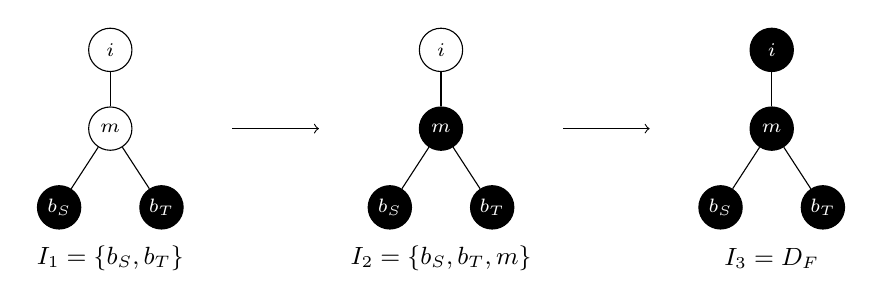
\begin{tikzpicture}[
  v/.style={circle,draw,minimum size=5.5mm,inner sep=0pt,font=\scriptsize},
  on/.style={v,fill=black,text=white},
  every edge/.style={draw}
]
  \begin{scope}[xshift=-4.2cm]
    \node[v] (i1) at (0,2) {$i$};
    \node[v] (m1) at (0,1) {$m$};
    \node[on] (b1) at (-.65,0) {$b_S$};
    \node[on] (c1) at (.65,0) {$b_T$};
    \draw (i1)--(m1); \draw (m1)--(b1); \draw (m1)--(c1);
    \node[font=\small] at (0,-.65) {$I_1=\{b_S,b_T\}$};
  \end{scope}
  \begin{scope}
    \node[v] (i2) at (0,2) {$i$};
    \node[on] (m2) at (0,1) {$m$};
    \node[on] (b2) at (-.65,0) {$b_S$};
    \node[on] (c2) at (.65,0) {$b_T$};
    \draw (i2)--(m2); \draw (m2)--(b2); \draw (m2)--(c2);
    \node[font=\small] at (0,-.65) {$I_2=\{b_S,b_T,m\}$};
  \end{scope}
  \begin{scope}[xshift=4.2cm]
    \node[on] (i3) at (0,2) {$i$};
    \node[on] (m3) at (0,1) {$m$};
    \node[on] (b3) at (-.65,0) {$b_S$};
    \node[on] (c3) at (.65,0) {$b_T$};
    \draw (i3)--(m3); \draw (m3)--(b3); \draw (m3)--(c3);
    \node[font=\small] at (0,-.65) {$I_3=D_F$};
  \end{scope}
  \draw[->] (-2.65,1) -- (-1.55,1);
  \draw[->] (1.55,1) -- (2.65,1);
\end{tikzpicture}
\caption{A flag of ancestry ideals for the running tree
\(i(m(b_S,b_T))\).  Black vertices have been exposed by that stage.  The
leaves \(b_S,b_T\) may exchange order, but the rule \(m\) cannot precede its
premises and \(i\) cannot precede \(m\).}
\label{fig:iterated-cut-flag}
\end{figure}

\begin{proof}
In the ideal form of the coproduct, an address-resolved iterated term has
successive tensor layers
\(I_1,I_2\setminus I_1,\ldots,D_F\setminus I_{n-1}\).
Conversely, successive frontier cuts of any flag produce a unique
address-resolved term; coassociativity identifies its parenthesisations.
Assigning each rule occurrence the first ideal in which it appears then
gives the weakly order-preserving map, and initial preimages give the
inverse flag.  Refining the flag until one new vertex is added at each
stage gives a linear extension of \(D_F\), and
Theorem~\ref{thm:linked-factorisation}(iv) reassembles its
one-vertex layers independently of exchanges of incomparable stages.
\end{proof}

This establishes presentation reconstruction and premise-ancestry
recovery.  The reconstruction claim concerns the uncollected,
address-indexed witnesses: ordinary iterated coproduct endpoints contain
the source forest itself, while collected tensors can identify distinct
addresses.  Theorem~\ref{thm:typed-faa} records every one-stage typed
context decomposition, including closed side proofs; iterated cuts
additionally retain where those stages occur in a chosen proof tree.  This
allows the construction to be compared precisely with causal trace
semantics.

\subsection{Refinement traces and causal incidence}

Fix an equipped calculus \(C=(\Base,\Rules)\).  A \emph{backward-refinement
history} of a finite context \(R\) is a sequence
\[
 \Box^G=R_0\longrightarrow R_1\longrightarrow\cdots
       \longrightarrow R_N=R
\eqtag\label{eq:refinement-history}
\]
in which one current puncture is replaced at each step by the rule corolla
occupying that address in \(R\).  The punctures of \(R\) itself are left
unrefined.  Thus every rule occurrence of \(R\) is introduced exactly once;
the nodeless identity has the unique empty history.  Let
\(\equiv_{\parallel}\) be generated by exchanging two adjacent steps which
refine distinct punctures already present before either step.  These are
exactly the exchanges covered by
Corollary~\ref{cor:strict-refinement-interchange}.
Write
\[
 \mathsf{Hist}_C(\mathbf H;G)
   =\coprod_{R\in\Ctx_C(\mathbf H;G)}\mathsf{Hist}_C(R),
\]
with histories taken up to the same coherent context isomorphisms as their
stages.

To state the coalgebraic comparison, let
\(H^{\mathbb Z}_{\mathsf{ForPos}}\) be the rooted-forest sub-Hopf algebra of
the standard Hopf algebra of finite posets
\cite{aguiarbergeronsottile2006}.  Its product is disjoint union and its
coproduct splits a poset into a downward-closed ideal and the complementary
upset:
\[
 \Delta_{\mathrm{inc}}[P]
   =\sum_{I\in J(P)}[I]\otimes[P\setminus I],
\eqtag\label{eq:forest-poset-incidence-coproduct}
\]
where \(J(P)\) is the set of downward-closed ideals and both factors carry
the induced order.  Empty factors give the two endpoints.  Write
\(H^{\mathbb Z}_{\Base,\Rules}\) for the integral form of the proof-tree
Hopf algebra.

For the orientation used here, a downward ideal of a rooted-forest ancestry
poset is a disjoint union of rooted descendant subtrees, while its
complementary upset is the remaining root-containing pruned forest.
Therefore these posets are closed under both factors of
\(\Delta_{\mathrm{inc}}\), which is why they form the stated sub-Hopf
algebra rather than merely a subspace of the poset Hopf algebra.

\begin{theorem}[Causal-trace representation and CK incidence semantics]
\label{thm:causal-ck-semantics}
Let \(R\) be a connected finite proof context and \(F\) a finite proof
forest.
\begin{enumerate}[label=(\roman*)]
\item Histories of \(R\) are reverse linear extensions of \(D_R\).  The
final-context map therefore induces a bijection
\[
 \mathsf{Hist}_{C}(\mathbf H;G)/{\equiv_{\parallel}}
       \ \cong\ \Ctx_C(\mathbf H;G),
\eqtag\label{eq:history-trace-quotient}
\]
where the left side ranges over histories ending in contexts of the
displayed interface.
\item If \(|V(R)|>0\), augment the CK cut choices of \(R\) by the whole-tree
endpoint.  For \(c\in\mathcal A(R)\), send \(c\) to the vertex region
detached by it,
\[
 I_c=\bigcup_{p\in c}V(R|_p),
\eqtag\label{eq:cut-ancestry-ideal}
\]
sends the empty cut to \(\varnothing\), sends the whole-tree endpoint to
\(D_R\), and gives a bijection with \(J(D_R)\).  For a nonempty proper
ideal, the inverse cut is its antichain of maximal elements.
\item Forgetting boundaries, rule tags, component data, and punctures but
retaining premise ancestry defines a graded Hopf map
\[
 \operatorname{Anc}:H^{\mathbb Z}_{\Base,\Rules}
      \longrightarrow H^{\mathbb Z}_{\mathsf{ForPos}},
 \qquad [F]\longmapsto[D_F].
\eqtag\label{eq:ancestry-hopf-map}
\]
Thus the proof-tree CK coproduct is a typed, proof-relevant lift of the
incidence coproduct of causal ideals.
\item Let \(\zeta([F])=1\) for every basis forest, and let
\[
 \omega_1([F])=
 \begin{cases}
 1,&|V(F)|=1,\\
 0,&|V(F)|\ne1.
 \end{cases}
\eqtag\label{eq:causal-characters}
\]
Then, for \(n\ge1\),
\[
 \zeta^{*n}([F])
   =\#\{f:D_F\to[n]\mid f\text{ is weakly order-preserving}\}.
\eqtag\label{eq:ck-order-polynomial}
\]
If \(N=|V(F)|>0\), then
\[
 \omega_1^{*N}([F])
       =|\operatorname{LinExt}(D_F)|.
\eqtag\label{eq:ck-linear-extension-count}
\]
For connected positive-degree \(R\), reversal gives a bijection between
\(\operatorname{LinExt}(D_R)\) and its root-first refinement histories, and
\[
 1+\mathsf{Cut}_R(q)
  =\sum_{A\in\operatorname{Ant}(D_R\setminus\{\rho_R\})}q^{|A|},
 \qquad
 \max_{c\in\mathcal A(R)}|c|
  =\operatorname{width}(D_R\setminus\{\rho_R\}).
\eqtag\label{eq:ck-causal-width}
\]
where \(\rho_R\) denotes the unique root occurrence of \(R\).
For a one-vertex context both sides of the width equation are \(0\).
\end{enumerate}
\end{theorem}

\begin{proof}
Label a refinement step by the address of the vertex it creates in the
final context.  A parent rule must already be present before a rule can be
inserted into one of its premise positions, so the resulting time order is
a reverse linear extension of \(D_R\).  Conversely, every reverse linear
extension gives a legal refinement sequence.  Any two linear extensions of
a finite poset are connected by adjacent exchanges of incomparable
elements; strict refinement interchange identifies exactly those exchanges.
This proves (i).

For \(c\in\mathcal A(R)\) with \(R\) of positive degree, the union in
\eqref{eq:cut-ancestry-ideal} is downward
closed.  Every proper ideal is the downward closure of its maximal
elements, which form a nonroot antichain; the empty and total ideals give
the two exceptional choices.  This proves (ii).

For a connected generator \(t\), part (ii) identifies every coproduct term,
including endpoints, with a unique ideal \(I\in J(D_t)\).  Writing \(c\)
for the associated cut choice, including the endpoint conventions,
\[
 D_{P^c(t)}=I,
 \qquad
 D_{R^c(t)}=D_t\setminus I.
\]
Thus \(\operatorname{Anc}\) preserves the coproduct on connected
generators.  Forest union becomes disjoint union of posets, so
multiplicativity extends the equality to every forest.  Connected
gradedness then gives the antipode compatibility and proves (iii).

The functional \(\zeta\) is a character and \(\omega_1\) is an
infinitesimal character.  Expanding an \(n\)-fold convolution expands the
iterated CK coproduct.  Proposition~\ref{thm:cut-flags} identifies its
address-resolved terms with weakly order-preserving maps to \([n]\), and
\(\zeta\) assigns \(1\) to every layer.  Requiring all \(N\) layers to have
degree one instead selects linear extensions and proves
\eqref{eq:ck-linear-extension-count}.  Finally, proper cuts are precisely
the nonempty antichains of nonroot vertices.  Every antichain occurs, so
the largest cut has the width stated in \eqref{eq:ck-causal-width}.
\end{proof}

The integer in \eqref{eq:ck-order-polynomial} is the order polynomial of
the presentation-ancestry poset evaluated at \(n\).  After base change to a
coefficient ring of positive characteristic it is observed modulo that
characteristic; address-indexed witnesses retain the individual schedules
before collection.  No rule name contributes to
\eqref{eq:ancestry-hopf-map}: decorations supply the typed proof-theoretic
lift, while the causal order is carried by CK cut support and convolution
multiplicity.

The history/linear-extension correspondence, the cut/ideal bijection, and
the resulting order-polynomial counts are standard trace and poset-Hopf
mechanisms.  Their role here is not a new concurrency theorem.  The
paper-specific content is their lift to typed proof contexts, where each
frontier retains a detached proof forest, a punctured filling interface,
material grounds, and hypersequent component data.

\begin{corollary}[Antipode reciprocity for causal stages]
\label{cor:causal-antipode-reciprocity}
Work over a characteristic-zero coefficient ring.  Let
\(\mathsf{ord}_{P}(x)\) be the order polynomial occurring in
\eqref{eq:ck-order-polynomial}, and let
\(\mathsf{ord}^{\circ}_{P}(n)\) count strictly order-preserving maps
\(P\to[n]\).  For \(N=|V(F)|\) and \(n\ge1\),
\[
 ((\zeta\circ S)^{*n})([F])
   =\mathsf{ord}_{D_F}(-n)
   =(-1)^N\mathsf{ord}^{\circ}_{D_F}(n).
\eqtag\label{eq:causal-antipode-reciprocity}
\]
Thus the convolution inverse supplied by the antipode performs the standard
incidence-Hopf inclusion--exclusion which replaces weak causal layerings by
signed strict layerings.  It is not a proof reduction or an inverse proof.
\end{corollary}

\begin{proof}
Put \(\eta=\zeta-\epsCK\).  This functional vanishes in degree zero and is
locally nilpotent for convolution on each fixed finite-degree forest.
Consequently the binomial identity
\[
 \zeta^{*m}([F])
   =\sum_{k\ge0}\binom{m}{k}\eta^{*k}([F])
\]
is degreewise finite.  Work first in the integral form.  For positive
integers \(m\) the left side is \(\mathsf{ord}_{D_F}(m)\) by
Theorem~\ref{thm:causal-ck-semantics}; the finite binomial expression and
the order polynomial are therefore the same polynomial over \(\mathbb Q\).
Evaluating that integer-valued identity at negative integers and then
extending scalars to the chosen coefficient ring gives the claimed
identity.  Since
\(\zeta\circ S=\zeta^{*-1}\), taking \(m=-n\) gives the first displayed
equality; compare the Hopf-algebraic treatment of poset chain enumerators
in \cite{ehrenborg1996}.  Stanley's order-polynomial reciprocity
\cite{stanley1972} gives the second equality.
\end{proof}

The trace principle itself is established concurrency mathematics.  Event
structures represent computations by event occurrences, causal
prerequisites, and conflict \cite{nielsenplotkinwinskel1981}; for a fixed
completed context, \(D_R\) is only the conflict-free event-poset part of
that picture, not a global event-structure semantics of proof search.
Benson's shuffle/cut bialgebras algebraise interleavings and word-like
traces \cite{benson1989}; their operations differ from the forest
juxtaposition and ancestry cutting used here.  More closely, Behr and Kock
identify reorderings of sequentially independent rewrites by shift
equivalence and construct a cocommutative Hopf algebra of causal tracelets
\cite{behrkock2022}; their coproduct splits a tracelet normal form into
subsets of primitive connected components.  The generally noncocommutative
coproduct here instead cuts within one proof-dependency tree and returns a
detached typed proof forest together with the punctured context which uses
it.  Castellan and Yoshida construct causal invariants for unit-free MALL
whose equality characterises commuting conversions
\cite{castellanyoshida2019}.  By contrast, \(D_R\) records explicitly
\emph{presentation causality}: the MLL obstruction below shows that raw CK
may retain ancestry forgotten by an accepted proof permutation.  Hopf
algebra has also entered denotational proof semantics through shuffle
actions used for noncommutative full completeness
\cite{blutescott1998}; that construction acts on denotations, whereas the
present CK basis consists of proof presentations and its coproduct
decomposes them.

This completes the central sequence from cut through the CK coproduct to
typed context composition and causal incidence.  We next apply it to
changes of material base before turning to proof identity.
\subsection{Persistent and revisory material change}

Material change affects the prospective side of the construction.  A
persistent extension leaves every old proof and its cuts untouched but may
supply new evidence for an old puncture.  Withdrawing a previously admitted
ground is different: affected proof presentations must be removed by a
quotient, after which their surviving contexts can expose replacement
obligations.

\begin{proposition}[Persistent material inclusion and filling]
\label{prop:base-extension}
Let \(\Base\subseteq\Base'\) be a persistent material inclusion,
preserving every old concrete occurrence.  Reinterpretation of an existing
\((\Base,\Rules)\)-proof as a \((\Base',\Rules)\)-proof commutes with
filling: for \(\mathbf t\in\Fill^{\Base,\Rules}(R)\),
\[
 j_*\!\left(\operatorname{ev}_{R}(\mathbf t)\right)
 \ \cong\
 \operatorname{ev}_{j_*R}(j_*\mathbf t).
\eqtag\label{eq:base-extension}
\]
Thus enlarging the material base may add positive-arity material rules as
well as nullary grounds, and hence new proofs, contexts, and possible
fillers, while preserving every puncture position and surrounding rule
context of an old proof.  Every filling operation anchored over the old
base is natural over its persistent extensions.
\end{proposition}

\begin{proof}
Every old occurrence remains in the enlarged calculus.  Both sides
substitute the same proofs into the same premise slots.
\end{proof}

\begin{definition}[Persistent calculus inclusion and conservativity]
\label{def:base-conservativity}
With the boundary language and colours fixed, a
\emph{persistent calculus inclusion}
\[
  \iota:(\Base,\Rules)\hookrightarrow(\Base',\Rules')
\]
consists of a persistent material inclusion together with
instance-preserving injections of the old logical initials and
concrete rule occurrences into the new ones.  These injections preserve
constructor tags, ordered premise positions, boundaries, component focus,
and derived component relations, and hence induce a recursive
reinterpretation map
\(\iota_*:\Prf_{\Base,\Rules}(G)\to
\Prf_{\Base',\Rules'}(G)\).

Given a class \(\mathcal C\) of old boundaries, the inclusion is
\emph{\(\mathcal C\)-consequence-conservative} when
\[
 \Prf_{\Base',\Rules'}(G)\ne\varnothing
 \quad\Longrightarrow\quad
 \Prf_{\Base,\Rules}(G)\ne\varnothing
 \qquad(G\in\mathcal C).
\eqtag\label{eq:consequence-conservativity}
\]
For a selected family \(D\) of constructor tags common to the two calculi,
write
\[
 \Prf_{\Base,\Rules}^{\neg D}(G)
   =\{t\in\Prf_{\Base,\Rules}(G):
          t\text{ contains no occurrence tagged }D\}.
\eqtag\label{eq:constructor-free-proof-fibre}
\]
The inclusion is \emph{\(D\)-free consequence-conservative} when the same
inhabited-fibre condition holds for the \(D\)-free subsets.  For the family
of formula-mediated Gentzen-Cut instances we say
\emph{Gentzen-Cut-free}.
\end{definition}

By \eqref{eq:closed-support-as-filling}, consequence conservativity
preserves inhabitedness of old one-puncture filling fibres while allowing
new proofs in them.  Premise nonmonotonicity instead concerns
\(\Gamma\mapsto\Gamma,\Upsilon\) inside one support relation.  A persistent
inclusion extends the stock of admitted evidence; a revisory change which
withdraws an old material occurrence is treated below by a quotient.
Thus the support relation may be nonmonotone in its formula premises while
the causal-incidence and resource-use results remain valid over every fixed
equipped calculus.  If adding information defeats an old ground, or if a negative rule
condition ceases to hold after extension, the change is not persistent and
no forward Hopf map is asserted.  The fixed-calculus theorems remain intact;
only naturality across that revisory change is unavailable.

The following theorem packages one repeated observation.  Calling the
assignment a \emph{functor} says only that reinterpreting an old proof along
successive persistent inclusions agrees with reinterpreting it once along
their composite.  The substantive claim is that this reinterpretation also
preserves every CK cut and filling operation.

\begin{theorem}[Persistent calculus inclusions and factorisation naturality]
\label{thm:base-hopf-functor}
Fix the boundary language \(\Lang\), and let
\(\mathsf{Calc}_{\Lang}\) be the category whose objects are equipped
calculi \((\Base,\Rules)\) and whose arrows are persistent calculus
inclusions from Definition~\ref{def:base-conservativity}.  The assignment
\[
 (\Base,\Rules)\longmapsto H_{\Base,\Rules},
\qquad
 \bigl(\iota:(\Base,\Rules)\hookrightarrow
                  (\Base',\Rules')\bigr)
 \longmapsto
 \bigl(\iota_*:[F]\mapsto[\iota_*F]\bigr)
\eqtag\label{eq:base-hopf-functor}
\]
is a functor to connected graded Hopf \(k\)-algebras and injective graded
Hopf maps.  At witness level, for every old proof \(t\) and CK cut
\(c\),
\[
\begin{aligned}
P^c(\iota_*t)&=\iota_*P^c(t),&
R^c(\iota_*t)&=\iota_*R^c(t).
\end{aligned}
\eqtag\label{eq:base-linked-naturality}
\]
Thus \(\iota_*\) identifies every old address-indexed and iterated cut, while
embedding its old evaluation family into the possibly larger filling
family in the extended calculus.
The maps also commute with \(\Root,\BRoot\) and typed filling.  Recursive
reinterpretation induces compatible
injections
\(
\OpenPrf_{\Base,\Rules}(X)\hookrightarrow
\OpenPrf_{\Base',\Rules'}(X)
\)
and hence inclusions on labelled punctured-context coefficients.

For fixed \(\Rules\), the subcategory in which only \(\Base\) varies is
the material-extension category
\(\mathsf{Mat}_{\Lang,\Rules}\).  The preceding functor restricts to the
material-base functor used below.
\end{theorem}

\begin{proof}
Injectivity of \(\iota\) on the full tagged constructor signature makes
\(\iota_*\) injective on
rule-rooted trees and forests.  An old proof has exactly the same vertex
order after reinterpretation.  Every prefix-free cut set therefore gives
the same detached and retained factors at the same addresses, proving
\eqref{eq:base-linked-naturality} and
\[
 \DeltaCK \iota_*=(\iota_*\otimes \iota_*)\DeltaCK,
 \qquad
 \epsCK \iota_*=\epsCK .
\]
Forest union and vertex degree are unchanged, so \(\iota_*\) is an injective
graded bialgebra map; connected gradedness makes it commute with the
antipodes.  Identity and composition of persistent inclusions act
identically on every old rule occurrence, proving functoriality.  The root
assertions are immediate.  The proof of
Proposition~\ref{prop:base-extension} applies verbatim: both sides insert
the same reinterpreted terms into the same preserved premise slots.
Recursive reinterpretation injects every old punctured proof and every
labelled context into the larger grammar; marking literal puncture
occurrences commutes with that inclusion, which gives the coefficient
inclusions.
\end{proof}

Logically, a persistent extension leaves the decomposition of every old
hypersequent proof unchanged.  It may only supply further proofs of premise
requirements already determined by the retained rule contexts.

\begin{corollary}[Base-extension naturality of proofs and filling]
\label{cor:proof-fibre-parametricity}
For each boundary \(G\), the assignment
\[
 \mathsf P_G(\Base)=\Prf_{\Base,\Rules}(G),
 \qquad
 \mathsf P_G(j)=j_*,
\]
defines a covariant functor
\(\mathsf P_G:\mathsf{Mat}_{\Lang,\Rules}\to\mathsf{Set}\).
Fix an anchor base \(\Base_\ast\), let
\(\mathsf{Ext}(\Base_\ast)\) be its category of persistent extensions, and
let \(R_\ast\) be an \(n\)-punctured derivation admitted over
\(\Base_\ast\), with root boundary \(G\) and labelled premise telescope
\((x_i:G_i)_{1\le i\le n}\).  For each persistent extension \(\Base\) of
\(\Base_\ast\), write
\(R_{\Base}\) for its reinterpretation.  Filling defines a natural
operation on this extension category,
\[
 \operatorname{ev}_{R_\bullet}
   =\bigl(\operatorname{ev}_{R_{\Base}}\bigr)_
         {\Base\in\mathsf{Ext}(\Base_\ast)}:
 \prod_i\mathsf P_{G_i}|_{\mathsf{Ext}(\Base_\ast)}
 \Longrightarrow
 \mathsf P_G|_{\mathsf{Ext}(\Base_\ast)} .
\eqtag\label{eq:proof-fibre-natural-operation}
\]
Explicitly, for every persistent inclusion
\(j:\Base\hookrightarrow\Base'\),
\[
 j_*\!\left(\operatorname{ev}^{\Base}_{R_{\Base}}(\mathbf t)\right)
 \cong
 \operatorname{ev}^{\Base'}_{R_{\Base'}}(j_*\mathbf t).
\eqtag\label{eq:proof-fibre-naturality}
\]
Every address-indexed cut and the collected coproduct of every old
evaluation are transported by the same reinterpretation.
\end{corollary}

\begin{proof}
The functor laws are those of recursive reinterpretation.  Equation
\eqref{eq:proof-fibre-naturality} is Proposition~\ref{prop:base-extension}
applied simultaneously to the displayed punctures.  Theorem
\ref{thm:base-hopf-functor} gives the factorisation assertions.
\end{proof}

Every old filling embeds into the corresponding filling set over a
persistent extension; additional fillers may become available while the
anchored operation and all its old factorisations are preserved.  This
naturality maps proofs forward along material-base extensions in the same
direction as the uniformity clauses of base-extension semantics, but its
values are proof presentations rather than support judgements.  The
discrete presentation in \eqref{eq:discrete-material-presentation}
resembles a sequent-based atomic system only at boundary level:
\(\Gamma\) is stored inside the nullary boundary
\(\Gamma\ms\Delta\), not exposed as a list of proof premises.  Positive
arity can represent primitive atomic rules with proof premises, but neither
presentation by itself defines semantic support.  This distinction is
especially relevant to recent sequent-calculus formulations of
base-extension semantics
\cite{sandqvist2015,barrosonascimentopiotrovskapimentel2026,
gheorghiuGuPymIMLL,guGheorghiuPymBI}.

A genuine adequacy result would additionally have to specify
\begin{enumerate}[label=(\alph*)]
\item the class of semantic atomic bases and their admissible extensions;
\item the atomic derivability relation generated at each base;
\item support clauses for the chosen logical vocabulary, including any
resource splitting and hypersequent bars;
\item soundness and completeness against inhabited proof fibres; and
\item when an operation natural over all base extensions is represented by
one anchored proof context.
\end{enumerate}
The last point is not formal: extension naturality alone may give a family
of support implications without selecting a single uniform context.  If an
independently defined semantics proves
\(
\Base\Vdash G\Longleftrightarrow
\Prf_{\Base,\Rules}(G)\ne\varnothing
\)
with the required resource indices, then an anchored context supplies the
forward extension-uniform implication from support of its premises to
support of its conclusion.  The missing converse would be a representation
theorem: every suitably natural support operation is induced by one
anchored context.  Proving items (a)--(d) and that representation theorem
in item (e) is additional proof-theoretic work, not a consequence of CK
naturality.  The fixed-calculus results also permit a support relation
nonmonotone in formula premises; a semantic change which defeats an old
ground is revisory rather than an arrow of the persistent extension
category.

At the one-hole level, context composition and filling already have the
familiar categorical shape.  Fix \(C=(\Base,\Rules)\), and write
\(\Prf_C,\Ctx_C\) for its proof and context families.  The one-hole sector
forms the category
\(\mathsf{Use}_C(H,G)=\Ctx_C(H;G)\), with puncture insertion as
composition and \(\Box^G\) as identity, and it acts covariantly on proof
fibres by filling.  Persistent calculus inclusions induce faithful
identity-on-objects functors between these categories and commute with
their actions.  This is the unary part of context composition, not a
category taking arbitrary derivations as arrows and formula-mediated
Gentzen Cut as composition.

The next result is an extensionality criterion for raw proof-context
presentation, not a proposed identity of proofs: distinctly tagged generic
fillers separate contexts.

\begin{theorem}[Generic-filler separation of proof contexts]
\label{thm:generic-filler-separation}
Let \(R,R'\in\Ctx_C(\mathbf H;G)\) be finite proof contexts with the
same root and a chosen alignment
\(\mathbf H=(x_1:H_1,\ldots,x_n:H_n)\) of all their punctures.  The
following are equivalent:
\begin{enumerate}[label=(\roman*)]
\item \(R\cong R'\) by an isomorphism inducing the chosen puncture
alignment;
\item for every persistent calculus extension
\(j:C\hookrightarrow C'\) and every compatible tuple
\(\mathbf t=(t_i)\) of complete \(C'\)-proofs,
\[
       (j_*R)[t_i/x_i]_i\cong(j_*R')[t_i/x_i]_i;
\eqtag\label{eq:all-filler-separation}
\]
\item the equality in \eqref{eq:all-filler-separation} holds in the one
persistent formal rule-signature extension \(C^\pi\) obtained by adjoining
pairwise distinct fresh nullary probe occurrences
\[
                  \pi_i:()\longrightarrow H_i
\]
and taking \(t_i=\pi_i()\).
\end{enumerate}
The probe tags are indexed by puncture labels, so equal requirements
\(H_i=H_j\) remain distinguishable.
\end{theorem}

\begin{proof}
Part (i) is preserved by reinterpretation and filling, giving (ii), and
(ii) gives (iii).  Conversely, every fresh tag \(\pi_i\) occurs exactly
once in each completed proof and nowhere in either old context.  An
isomorphism in (iii) must preserve that tag, hence its label \(x_i\) and,
when it is nonroot, its parent premise slot.  Removing the matched probe
leaves (or restoring the root identity context) recovers an isomorphism
\(R\cong R'\) inducing the chosen alignment.
\end{proof}

The theorem makes filling jointly separating over persistent extensions:
a raw punctured proof presentation is determined by its uniform action on
possible reasons, and one finite tuple of generic reasons suffices.  The
probe extension is metasyntactic and need not be consequence-conservative.
This is generic-element separation in the free proof-term grammar: under
a faithful Curry--Howard assignment the same fresh constants separate
typed term contexts.  It is a syntactic genericity result, not relational
parametricity.
Proof identity coarser than presentation is treated below by quotienting
the same context-composition operations.

Write \(\Sigma_{\Base,\Rules}\) for the full tagged signature of material
occurrences, logical initials, and admitted logical or structural rule
instances.  For any tagged constructor signature \(\Sigma\), write
\(H_\Sigma\) for its proof-tree Hopf algebra.  If \(D\) is a selected
family of material, logical, or structural constructor tags, let
\[
 I_D=\operatorname{span}_k\{[F]:F\text{ contains an occurrence tagged by }D\}.
\eqtag\label{eq:constructor-deletion-ideal}
\]

An algebra ideal is called a \emph{Hopf ideal} when coproduct, counit, and
antipode pass to the quotient.  Equivalently for the present connected
graded setting, cutting an element of the ideal always leaves at least one
tensor factor in the ideal, and the counit vanishes there.  The next result
is the standard decorated-tree instance of that condition; its
proof-theoretic use follows the statement.

\begin{theorem}[Constructor deletion as a Hopf quotient]
\label{thm:constructor-deletion}
The subspace \(I_D\) is a homogeneous Hopf ideal, and deletion of the
tagged instances induces
\[
 H_{\Sigma_{\Base,\Rules}}/I_D
   \ \cong\
 H_{\Sigma_{\Base,\Rules}\setminus D}.
\eqtag\label{eq:constructor-deletion-hopf-quotient}
\]
\end{theorem}

This is the standard decorated-tree constructor-ideal result
\cite{foissy2002,foissy2021typed}: a CK cut places every selected vertex
in one of its two factors, and the surviving forest basis is precisely
the basis over the signature with \(D\) deleted.

Its use below is proof-theoretic: constructor deletion lets full and
selected proof fibres be compared without identifying either with mere
derivability support.

\begin{corollary}[Effect on filling fibres]
\label{cor:constructor-deletion-filling}
For every \(D\)-free punctured proof \(R\), constructor deletion restricts
its filling fibre to the tuples whose completed proof contains no
occurrence tagged by \(D\).  In particular, when \(D\) is the family of
Gentzen-Cut instances, the quotient is the Hopf algebra of
Gentzen-Cut-free proof presentations.
\end{corollary}

A completed filling is \(D\)-free exactly when its fixed context and all
its fillers are \(D\)-free.

The quotient gives a retrospective answer: it removes a proof
presentation once a forbidden constructor has been found in it.  There is
also a prospective question---which proof contexts can be built without
that constructor in the first place?  The ordinary recursive grammar of
proof trees answers it by the following standard polynomial fixed point.

\begin{corollary}[Prospective constructor-free grammar]
\label{prop:constructor-truncation-dse}
Let
\(\Sigma^-=\Sigma_{\Base,\Rules}\setminus D\), and let
\(P^-\) be the many-sorted polynomial
\eqref{eq:proof-polynomial} with the \(D\)-tagged constructor summands
deleted.  Let \(q_D\) be the quotient map of
Theorem~\ref{thm:constructor-deletion}.  Write
\(\mathcal O_{\Sigma^-}\) for the typed proof contexts
over this truncated signature and put
\[
 W_G^-=\coprod_{\mathbf K\in\HSeq^\ast}
          \mathcal O_{\Sigma^-}(\mathbf K;G).
\]
Let \(\mathsf{Id}_G=\{\Box^G\}\) and let
\(\mathsf{Id}=(\mathsf{Id}_G)_{G\in\HSeq}\) be the many-sorted family of
identity contexts.  Final-root decomposition gives the initial-algebra
equation
 \[
                 W^-\cong\mathsf{Id}+P^-(W^-).
\eqtag\label{eq:constructor-truncation-dse}
\]
This is the ordinary recursive constructor-free proof grammar (or,
equivalently, its standard many-sorted combinatorial Dyson--Schwinger
equation) \cite{kock2017}.  For every positive-vertex
basis proof or context \(T\),
\[
 T\text{ is \(D\)-free}
 \quad\Longleftrightarrow\quad
 T\in W^-
 \quad\Longleftrightarrow\quad
 q_D[T]\ne0 .
\eqtag\label{eq:constructor-free-three-way}
\]
Define its profile-refined Green family by
\[
 \mathfrak N_{\mathbf K}^{G,-}
   =\delta_{\mathbf K,(G)}\one+
      \sum_{C\in\mathcal O_{\Sigma^-}^+(\mathbf K;G)}[C].
\]
Under the quotient identification of
Theorem~\ref{thm:constructor-deletion},
\[
             q_D(\mathfrak G_{\mathbf K}^{G})
                =\mathfrak N_{\mathbf K}^{G,-};
\]
applying \(q_D\otimes q_D\) to
\eqref{eq:typed-operadic-faa} gives the same identity with every
\(\mathfrak G\) replaced by \(\mathfrak N^{-}\), without a new
combinatorial proof.
\end{corollary}

The quotient is retrospective: it rejects a presentation in which a
deleted constructor occurs.  The fixed point is prospective: it enumerates
the contexts still available to proof search.  For
\(D=\mathrm{GCut}\), the support of
\(\mathfrak N_{()}^{G,-}\) is precisely the complete
Gentzen-Cut-free \(G\)-proof fibre.  Neither construction rewrites a
rejected proof; typed reducts, termination, and confluence remain data of
the underlying calculus.

\begin{corollary}[Material withdrawal and revision]
\label{thm:material-withdrawal}
If \(D\subseteq\Base\) is a subfamily of material occurrences, then
\[
 H_{\Base,\Rules}/I_D
   \ \cong\
 H_{\Base\setminus D,\Rules}.
\eqtag\label{eq:withdrawal-hopf-quotient}
\]
More generally, if
\(
 \Base=\Base_{\mathrm{keep}}\sqcup D
 \rightsquigarrow
 \Base'=\Base_{\mathrm{keep}}\sqcup A
\)
with common occurrences carrying identical concrete instances, the change factors as
\[
 H_{\Base,\Rules}
   \twoheadrightarrow
 H_{\Base_{\mathrm{keep}},\Rules}
   \hookrightarrow
 H_{\Base',\Rules}.
\eqtag\label{eq:revision-quotient-inclusion}
\]
The composite sends a proof using \(D\) to \(0\); alternative evidence is
described separately by the replacement context below.
\end{corollary}

This combines constructor deletion with the persistent inclusion
\(\Base_{\mathrm{keep}}\hookrightarrow\Base'\) of
Theorem~\ref{thm:base-hopf-functor}.

\begin{theorem}[Ground withdrawal exposes a replacement context]
\label{thm:ground-repair-fibre}
Let \(D\subseteq\Base\) be a finite family of tagged nullary material
occurrences,
and let \(t\) be a connected complete proof which uses \(D\) but is not
itself a one-vertex \(D\)-ground.  The occurrences
\[
 L_D(t)=\{v\in V(t):a_v\in D\}
\]
where \(a_v\) is the concrete rule occurrence decorating \(v\), form a CK
cut.  We identify a nullary occurrence \(a_v\) with its one-vertex
proof term \(a_v()\).
Cutting there detaches the \(D\)-grounds and
leaves the \(D\)-free punctured derivation \(\operatorname{Rep}_D(t)\):
\[
 \left[\mathop{\fjoin}_{v\in L_D(t)}a_v\right]\otimes
       [\operatorname{Rep}_D(t)] .
\eqtag\label{eq:ground-repair-coefficient}
\]
At each address \(v\), the requirement is
\(\Req_{\operatorname{Rep}_D(t)}(v)=\operatorname{out}(a_v)\).  If
\(\Base'=(\Base\setminus D)\sqcup A\) is a revised base, then
\[
 \Fill^{\Base',\Rules}
       (\operatorname{Rep}_D(t))
 \ \cong\
 \prod_{v\in L_D(t)}
       \Prf_{\Base',\Rules}(\operatorname{out}(a_v)).
\eqtag\label{eq:ground-repair-fibre}
\]
The bijection is natural under further persistent base inclusions.
\end{theorem}

\begin{proof}
Nullary grounds are leaves, so their distinct nonroot occurrences are
incomparable.  The CK cut at those occurrences replaces them by punctures
at the same addresses
and detaches exactly the displayed forest.  A filling is therefore
precisely an independent tuple of proofs with the required boundaries;
restriction to the inserted subtrees is the inverse.  Filling by the original
grounds reconstructs \(t\), and Proposition~\ref{prop:base-extension}
gives naturality.
\end{proof}

The quotient of Theorem~\ref{thm:constructor-deletion} says which old proofs
survive withdrawal; this theorem retains more intensional information about
an affected proof.  Its detached-ground factor presents a proof-replacement
obligation whose possible solutions are determined by the revised material
base.

Restricting every connected boundary and rule instance to singleton
hypersequents recovers the ordinary sequent-proof sector.  It is closed
under CK cuts, filling, and iterated cuts and therefore spans
a Hopf subalgebra.  The Communication occurrence studied in
Section~\ref{sec:communication}, whose conclusion has two active
components, marks the proper hypersequent extension.

Proof identity is supplied independently in the next section.

\section{Structural profiles and proof identity}
\label{sec:identity}

Keep three levels distinct.
\begin{enumerate}[label=(\roman*)]
\item \emph{Proof grammar.}  Weakening, Contraction, Splitting,
Communication, and similar admitted rules are concrete proof vertices.
Internal and external Exchange are instead absorbed by the multiset and
coherent-reindexing conventions.
\item \emph{Proof conversion.}  The proof theory may independently accept
conversions or equations between presentations.
\item \emph{Factorisation.}  The CK coproduct descends to the resulting
proof classes only when cutting equivalent representatives gives
equivalent collected factors---the coideal condition formalised below.
\end{enumerate}
Neither CK multiplication nor the CK coproduct is a structural rule.
Multiplication juxtaposes independent proof blocks; the coproduct opens a
proof presentation already built.

For any basis span \(M\) of proof forests, including a
constructor-deletion quotient identified with its surviving forest basis,
write \(M^{\mathrm{cl}}\) for the span of complete forests and
\(M_{\mathrm{cl}}^{\mathrm{con}}[G]\) for the span of connected complete
proofs with root boundary \(G\).

\subsection{Connected proof and independent forest}

The block-root profile from \eqref{eq:two-root-profiles} distinguishes a
connected proof of \(S\mid T\) from a forest containing independent proofs
of \(S\) and \(T\), even though their flattened boundaries agree.

\begin{proposition}[Connected realisation is not forest factorisation]
\label{thm:connected-factorised}
Let \(z\) be a one-vertex connected proof of \(S\mid T\), and let \(x,y\)
be distinct one-vertex proofs of \(S,T\).  Then
\[
 \Root(z)=\Root(x\fjoin y)=S\mid T,\qquad
 \BRoot(z)=\{S\mid T\}\ne\{S,T\}=\BRoot(x\fjoin y),
\]
while
\[
\begin{aligned}
 \DeltaCK[z]&=[z]\otimes\one+\one\otimes[z],\\
 \DeltaCK[x\fjoin y]&=[x\fjoin y]\otimes\one
                 +\one\otimes[x\fjoin y]
                 +[x]\otimes[y]+[y]\otimes[x] .
\end{aligned}
\eqtag\label{eq:connected-factorised}
\]
Consequently the equation \([z]=[x\fjoin y]\) does not preserve CK factorisation over
a nonzero coefficient ring.
\end{proposition}

\begin{proof}
One-vertex connected trees are primitive and the coproduct is
multiplicative.  Modulo \([z]-[x\fjoin y]\), the endpoint terms cancel while the two
mixed tensors remain.  They record the separate detachability of the forest
factors.
\end{proof}

Forest multiplication is therefore vertex-free juxtaposition, whereas an
admitted assembly rule contributes a connected vertex and its own cut.
Proof-theoretically, the former says only that two proofs are being
considered side by side; the latter records that the calculus performed a
specific operation on them.  This distinction is finer than the
hypersequent displayed at the root.  We call an admitted binary occurrence
\[
 \mathrm{Asm}_{\mid}:(\mathcal G,\mathcal H)
       \longrightarrow\mathcal G\mid\mathcal H
\eqtag\label{eq:bar-assembly-occurrence}
\]
a \emph{connected bar-assembly}: it joins two premise proofs below one
rule vertex and transports their displayed components bijectively.

To observe all cuts while keeping the root-containing proof context in a
distinguished position, remove the whole-tree endpoint from the
coproduct.  This is the role of a \emph{coaction}: it is bookkeeping for a
decomposition with one factor still living in the chosen space of rooted
proofs, not a further rule of the calculus.  For a hypersequent \(G\), let
\(C_G^{\mathrm{con}}\) be the span of connected rule-rooted derivation
trees, complete or punctured, with boundary \(G\), and let
\(C_G^{\mathrm{cl}}\subseteq C_G^{\mathrm{con}}\) be the subspace spanned by
the complete ones.  Put
\[
 \delta_G:C_G^{\mathrm{con}}\longrightarrow
     \HCK\otimes C_G^{\mathrm{con}},\qquad
 \delta_G[t]=\DeltaCK[t]-[t]\otimes\one .
\eqtag\label{eq:root-coaction}
\]
Every right-hand retained factor in \(\delta_G[t]\) still has root \(G\).
Formally, a left \(\HCK\)-coaction is a map
\(\delta:C\to\HCK\otimes C\) satisfying
\[
 (\DeltaCK\otimes\mathrm{id})\delta
   =(\mathrm{id}\otimes\delta)\delta,\qquad
 (\epsCK\otimes\mathrm{id})\delta=\mathrm{id}.
\]
These equations say that staged observation is coherent and that the empty
detached factor changes nothing.  Coassociativity and the counit law for
\(\DeltaCK\) give them for \(\delta_G\).  A space equipped with such a map
is called a \emph{comodule}; a comodule map preserves the observation.

\subsection{Local structural action of rule vertices}
\label{subsec:structural-footprints}

Component-local logical rules, internal structural rules, and external
hypersequent rules all occur as concrete connected vertices.  Their
behaviour is read from the instantiated rule and its component focus rather
than from the spelling of the tag.  For
\(G\in\HSeq\), let \(\br(G)\) be its number of displayed components.
For
\(
 a:(G_1,\ldots,G_{n(a)})\to G
\)
define its proof-factor and hypersequent-component defects by
\[
 \sigma_{\mathrm{pf}}(a)=1-n(a),
 \qquad
 \sigma_{\mathrm{hs}}(a)
   =\br(G)-\sum_{i=1}^{n(a)}\br(G_i).
\eqtag\label{eq:local-structural-defects}
\]
The first counts how many proof factors a rule joins beneath one root; the
second counts its net change in displayed hypersequent components.  The
derived relation \(\kappa_a\) in \eqref{eq:component-relation} records the
non-scalar movement, merger, splitting, deletion, or creation of component
occurrences.  Active and principal formula behaviour is already part of the
concrete instance \(a\) and need not be duplicated in the CK carrier.

The following familiar cases show what the two numbers see and why the
relation \(\kappa_a\) is also needed.
\begin{center}
\small
\begin{tabular}{@{}L{4.4cm}ccL{7.2cm}@{}}
\toprule
concrete rule occurrence & \(\sigma_{\mathrm{pf}}\) &
 \(\sigma_{\mathrm{hs}}\) & further incidence needed\\
\midrule
binary component-local logical rule (singleton-hypersequent boundaries) & \(-1\) & \(-1\) &
 active/principal formula in the concrete instance\\
connected bar-assembly & \(-1\) & \(0\) &
 two premise blocks assembled below one root\\
Communication (Section~\ref{sec:communication}) & \(-1\) & \(0\) &
 formula-occurrence-bijective but crossed component transport\\
unary Splitting & \(0\) & \(+1\) &
 one-to-many component transport\\
external Weakening adding one component & \(0\) & \(+1\) &
 unsupported output component\\
external Contraction & \(0\) & \(-1\) &
 many-to-one component or occurrence incidence\\
\bottomrule
\end{tabular}
\end{center}

The scalar pair checks boundary arithmetic.  Explicit connected
bar-assembly and separated-tail Communication have the same pair, while
their component relations distinguish independent assembly from crossed
transport.  External Exchange is the coherent reindexing already built
into hypersequent component occurrences.  If a binary component-local
instance repeats \(g\) passive components in both premises, then
\(\sigma_{\mathrm{hs}}=-(g+1)\); the first row records only the
singleton-boundary calibration \(g=0\).

\begin{lemma}[Euler form of the scalar defects]
\label{lem:euler-defects}
Let \(R\) be a nonempty finite punctured proof forest with
\(r\ge1\) connected roots.
Then
\[
\begin{aligned}
 \sum_{v\in V(R)}\sigma_{\mathrm{pf}}(a_v)
   &=r-|\Punc(R)|,\\
 \sum_{v\in V(R)}\sigma_{\mathrm{hs}}(a_v)
   &=\br(\Root R)-\sum_{p\in\Punc(R)}\br(\Req_R(p)).
\end{aligned}
\eqtag\label{eq:euler-defects}
\]
Thus the total scalar defects are determined by the root and premise
telescope.  Their useful intensional information is their distribution
among rule vertices and ancestry layers; the non-scalar component action
lies in \(\kappa\).
\end{lemma}

\begin{proof}
The premise edges between rule vertices number \(|V(R)|-r\), and the
remaining premise positions are the \(|\Punc(R)|\) punctures.  Hence
\(\sum_v n(a_v)=|V(R)|-r+|\Punc(R)|\), proving the first equation.  In the
second, the breadth of every internal premise boundary occurs once with a
minus sign at its parent and once with a plus sign at the child root; only
the forest roots and puncture requirements remain.
\end{proof}

For the empty forest, put
\(V(\one)=\Punc(\one)=\varnothing\) and
\(\br(\operatorname{flat}\varnothing)=0\); both identities then extend
to \(r=0\).  There is no nonempty root-free forest of nodeless context
identities in the CK carrier, because \(\Box^G\) is an identity for context
composition rather than a forest generator.

Accordingly, the carrier records component-local formula action through
active and principal incidence, internal structural action through
multiset-context incidence, and external structural action through
component transport.  Any nonnullary rule also joins its premise proof
blocks beneath a new vertex, so these recorded behaviours may overlap.
Whether a rule family is logical or harmonious is determined independently
by its substitution, inversion, and use behaviour.

For a relation \(L\subseteq X\times Y\), \emph{functional} means that each
\(x\) is related to at most one \(y\), \emph{inverse-functional} that each
\(y\) has at most one antecedent \(x\), \emph{total} that every \(x\) has
an image, and \emph{surjective} that every \(y\) has an antecedent.
Functionality forbids one-to-many splitting, inverse-functionality forbids
many-to-one merger, totality forbids erasure, and surjectivity forbids
unsupported creation.

For a punctured derivation \(R\), its \emph{composite component trace}
\(\kappa_R\) is obtained by putting identity relations at its punctures
and composing the local component relations \(\kappa_a\) towards the root.
Thus, for a root occurrence \(a\),
\[
 \kappa_{a(R_1,\ldots,R_{n(a)})}
   =\kappa_a\circ\bigsqcup_{i=1}^{n(a)}\kappa_{R_i}.
\eqtag\label{eq:structural-trace-recursion}
\]
Also put
\[
 \sigma_\bullet(R)=\sum_{v\in V(R)}
       \sigma_\bullet(a_v),
 \qquad
 \bullet\in\{\mathrm{pf},\mathrm{hs}\}.
\eqtag\label{eq:composite-scalar-defect}
\]

\begin{lemma}[Composition of component traces]
\label{thm:structural-footprints}
Let \(R\) be a punctured derivation with labelled positions
\(x_j:K_j\), where \(K_j=\Req_R(p_j)\) is inferred from the corresponding
slot position, and let \(t_j\) be compatible proof contexts, including
complete proofs as the filling case.  Then
\[
\begin{aligned}
 \kappa_{R\langle t_j\rangle}
   &=\kappa_R\circ\bigsqcup_j\kappa_{t_j},\\
 \sigma_\bullet(R\langle t_j\rangle)
   &=\sigma_\bullet(R)+\sum_j\sigma_\bullet(t_j),
 &&\bullet\in\{\mathrm{pf},\mathrm{hs}\}.
\end{aligned}
\eqtag\label{eq:structural-footprint-composition}
\]
Consequently a composite of functional traces cannot split an input, a
composite of inverse-functional traces cannot merge two inputs, a composite
of total traces cannot erase one, and a composite of surjective traces
cannot create an unsupported output.
\end{lemma}

\begin{proof}
Structural induction substitutes each filler trace at the identity trace of
its puncture.  Relational composition preserves the four stated properties,
and the vertex sets of the outer context and fillers are disjoint.
\end{proof}

\begin{proposition}[Occurrence-resolved component semantics]
\label{prop:component-relational-semantics}
Let \(\widetilde{\HSeq}\) be the family of hypersequent boundaries with
displayed component occurrences resolved, and let
\(\widetilde{\mathcal O}\) be the corresponding lift of the context
family before coherent reindexing.  For
\[
 C\in\widetilde{\mathcal O}((K_1,\ldots,K_n);G)
\]
put
\[
 \widetilde\kappa_C\subseteq
 \left(\bigsqcup_{i=1}^n\{i\}\times\Comp(K_i)\right)
 \times\Comp(G).
\eqtag\label{eq:occurrence-resolved-kappa}
\]
Then \(C\mapsto\widetilde\kappa_C\) preserves typed identities and
context composition:
\[
 \widetilde\kappa_{D\langle C_1,\ldots,C_m\rangle}
   =
 \widetilde\kappa_D\circ
       \bigsqcup_{j=1}^m\widetilde\kappa_{C_j}.
\eqtag\label{eq:kappa-context-morphism}
\]
Consequently, equality of \(\widetilde\kappa\)-relations is a typed
context congruence.  Persistent calculus inclusions preserve and reflect
this congruence on old contexts.
\end{proposition}

This is the composition equation of
Lemma~\ref{thm:structural-footprints} before coherent reindexing;
persistence fixes every old local relation and hence its composite.

\begin{corollary}[Local-to-global component-action criterion]
\label{cor:local-global-component-action}
Fix a family \(\mathcal S\) of concrete rule occurrences and generate
all compatible derivations from their full-premise corollas and typed
identities, including the complete corollas of nullary occurrences.  For
each property
\[
 \mathcal P\in
 \{\text{functional},\text{inverse-functional},
   \text{total},\text{surjective}\},
\]
every generated derivation has a \(\mathcal P\)-component trace if and only
if every \(\kappa_a\), \(a\in\mathcal S\), has property \(\mathcal P\).
The equivalence is invariant under coherent component reindexing.
\end{corollary}

\begin{proof}
The forward direction evaluates the claim on the full-premise corolla
\(\operatorname{Cor}(a)\), whose trace is \(\kappa_a\).  The reverse
direction is Lemma~\ref{thm:structural-footprints}, since disjoint union
and relational composition preserve each displayed property.
\end{proof}

For a complete proof the trace domain is empty.  Functionality,
inverse-functionality, and totality are therefore vacuous; surjectivity may
still detect an output component with no premise-component source.
Corollary~\ref{cor:local-global-component-action} concerns every derivation
generated by a rule family.  It does not classify a single composite: a
nonfunctional local trace may be followed by a rule whose net composite is
functional.

A coherent reindexing only renames input and output component occurrences,
so the carrier remembers the relation only up to those renamings.  This is
the invariance used by the CK-resolved profile below.

Identifying contexts exactly when their net component relations agree,
after coherent renaming, gives the compositional abstraction which forgets
everything except component transport.  It is not by itself an identity of proofs:
its nullary sector identifies all complete proofs of one root because their
relation has empty domain.  Any extension to forest equations must still
pass the CK coideal criterion if recursive factorisation is to survive.

By Lemma~\ref{lem:euler-defects}, total scalar defects are boundary data.
Their local distribution is a consistency check, while the composed
relations carry the non-scalar component action.
\[
\begin{array}{c@{\qquad}c}
\text{behaviour visible in }\kappa_R
&
\text{some local rule trace }\kappa_a\text{ must be}\\
\hline
\text{one input reaches two outputs} & \text{nonfunctional}\\
\text{two inputs reach one output} & \text{not inverse-functional}\\
\text{an input disappears} & \text{nontotal}\\
\text{an output has no source} & \text{nonsurjective}
\end{array}
\eqtag\label{eq:component-trace-payoff}
\]
Thus a composite proof context cannot acquire splitting, merger, erasure,
or unsupported creation merely by nesting otherwise incidence-preserving
rules.  The trace locates the kind of local structural action which must
occur somewhere in its ancestry.

\begin{proposition}[CK-resolved component profile]
\label{prop:ck-component-profile}
Let \(t\) be a connected complete proof.  For each proper CK cut \(c\),
let
\[
 Q_c=\bigsqcup_{p\in c}\{p\}\times
       \Comp(\rootseq(t|_p)),
 \qquad O_t=\Comp(\rootseq(t)).
\]
The cut addresses identify \(Q_c\) with the component occurrences expected
at the punctures of \(R^c(t)\).  Composing through the retained derivation
gives
\[
                  \kappa_t^c\subseteq Q_c\times O_t .
\]
The addressed family, called the \emph{CK-resolved component profile},
\[
 \mathsf{CT}(t)
   =\{(c,Q_c,\kappa_t^c,O_t):c\in\mathcal A^+(t)\}
\eqtag\label{eq:ck-component-profile}
\]
is unchanged by coherent reindexing of multiset-occurrence
representatives.  Forgetting the relations and
replacing each cut by \(q^{|c|}\) recovers
\(\mathsf{Cut}_t(q)\).  If the final occurrence \(a\) has at least one premise and
\(c_{\mathrm{fin}}\) consists of the roots of its immediate children, then
\[
                  \kappa_t^{c_{\mathrm{fin}}}\cong\kappa_a
\eqtag\label{eq:transport-final-corolla}
\]
under the ordered-premise identification.  Under context composition,
every retained relation is obtained by the composite law of
Lemma~\ref{thm:structural-footprints}.
\end{proposition}

\begin{proof}
The cut positions supply the domain, and recursive trace composition gives
\(\kappa_t^c\).  At the immediate-child cut the retained context is
the one-vertex final corolla, giving \(\kappa_a\).  Reindexing invariance
and the context-composition claim follow from coherent reindexing and
relational composition.
\end{proof}

\begin{corollary}[Persistent naturality of the CK-resolved profile]
\label{cor:component-profile-naturality}
Let
\(\iota:(\Base,\Rules)\hookrightarrow(\Base',\Rules')\)
be a persistent calculus inclusion and let \(t\) be an old complete
proof.  Under the canonical identification of its preserved boundary
component occurrences,
\[
                    \mathsf{CT}(\iota_*t)=\mathsf{CT}(t).
\]
Thus extension preserves not only every old cut and retained context but
also the component relation observed at that cut.
\end{corollary}

\begin{proof}
Theorem~\ref{thm:base-hopf-functor} preserves the cut addresses and both
CK factors.  Persistence preserves every old local relation
\(\kappa_a\); Lemma~\ref{thm:structural-footprints} therefore gives the
same composite \(\kappa_t^c\) for each cut.
\end{proof}

This couples a component relation to the CK location at which it is
observed.  A persistent extension may add new fillers and new contexts,
but it cannot reroute the components of an old proof at any old CK cut.
Final-corolla extraction and fully refined iterated cuts expose the full
concrete rule instance together with its causal position.  The collected CK
tensors are their coarser linear image.

\subsection{Rule application, conversion, and structural equations}

At the level of an individual rule, distinguish three operations.
\begin{enumerate}[label=(\roman*)]
\item \emph{Rule application.}  For an admitted occurrence \(e\),
\(B_e^+(\mathbf t)=e(\mathbf t)\) adds \(e\) as a new root below its
ordered premise proofs.  In the unary case this is the one-slot insertion
of \eqref{eq:unary-rooting-prelie}; higher arity uses simultaneous typed
composition.
\item \emph{Conversion.}  A proof conversion replaces one realised rule
context \(F\) by another \(F'\), transporting punctures, component indices,
and the fillings available in the fixed calculus.
\item \emph{Equation.}  Declaring \([F]=[F']\) symmetrically and
contextually generates an algebra ideal.  Whether the CK coproduct descends
to the resulting proof classes is a further question.
\end{enumerate}

The distinction is already exact for a unary occurrence \(e:G\to H\).  The
root-preserving coactions satisfy the affine recursion
\[
 \delta_H[B_e^+(t)]
   =(\mathrm{id}\otimes B_e^+)\delta_G[t]
       +[t]\otimes[\operatorname{Cor}(e)].
\eqtag\label{eq:affine-rule-grafting}
\]
The first summand transports every cut internal to the premise; the second
is the unique new cut immediately below \(e\).  A conversion which
preserves this collected root-preserving decomposition instead intertwines
the two coactions---that is, it is a comodule map---and has no extra
corolla term.
Formula \eqref{eq:affine-rule-grafting} applies without changing its form to a
unary component-local logical rule, internal structural rule, Splitting, external
Weakening, or external Contraction.  Binary Communication and explicit
connected bar-assembly obey the corresponding multi-input grafting
recursion, whereas definitional forest juxtaposition obeys multiplicativity.

Internal Exchange is absorbed by the multiset formula contexts.  External
Exchange acts by coherent reindexing of the component occurrences of a
hypersequent multiset.  Neither operation forgets the indexed premise order
of a proof rule: left and right inputs remain distinct unless that
particular rule schema carries an explicit input symmetry.  The connected
bar-assembly occurrence used below remains a connected rule vertex;
identifying its application with independent juxtaposition would be a
further equation subject to the coideal criterion.

\subsection{Proof congruences and the coideal diagnostic}

By puncture factorisation, the CK coproduct records decompositions into
detached proof forests and retained proof contexts.  If an equation is
intended to preserve this collected factorisation, the coproduct must be
independent of the chosen representative.  That requirement is precisely
coideal descent.  Algebraically, ``coideal'' names the condition that the
coproduct of every equation lies in
\(I\otimes\Hlic+\Hlic\otimes I\), where \(I\) is the generated equation
ideal, so it becomes zero after both tensor
factors are quotiented.  In
proof-theoretic terms, an equation passes the
coideal test exactly when it remains valid after either side is inspected
as detached evidence together with the punctured context which used it.
An identity intended to abstract from a chosen scheduling presentation need not
meet it; failure then diagnoses the dimension forgotten rather than
refuting the identity.

Proof identity is supplied independently; the Hopf structure tests its
factorisation stability.

\begin{definition}[Proof congruence]
\label{def:proof-congruence}
A \emph{compatible input labelling} of punctured forests \(F,F'\) is a
finite set \(I\) with bijections
\(\ell_F:I\to\Punc(F)\) and
\(\ell_{F'}:I\to\Punc(F')\) such that
\[
 \Req_F(\ell_F(i))=\Req_{F'}(\ell_{F'}(i))
 \qquad(i\in I).
\]
An \emph{aligned proof equation} consists of two forests admitted by the
fixed calculus, with the
same flattened root and, when they are punctured, a chosen compatible
input labelling.  The chosen labelling aligns common variables across
differently shaped contexts; it is not an intrinsic name on either proof
edge.

A \emph{proof congruence} \(E\) is the equivalence relation
\(\sim_E\) on the underlying unlabelled forests generated by a family of
aligned proof equations and their instances under forest multiplication,
uniform substitution of formula and context metavariables whenever the
resulting concrete occurrences remain in the calculus, and compatible context
composition along the specified alignments, hence in particular complete
filling.  The
alignment is retained while contextual instances are formed and then
forgotten on the CK basis.  Thus different alignments of equal-requirement
punctures need not generate the same equation.  Put
\[
 I_E=\operatorname{span}_k
       \{[F]-[F']:F\sim_EF'\}\subseteq\Hlic .
\eqtag\label{eq:proof-congruence-ideal}
\]
No preservation of vertex number or block-root profile is assumed.
\end{definition}

Flattened root is nevertheless invariant under every proof congruence.
Aligned generators have equal flattened root; forest multiplication adds the
same companion boundary to both sides, context composition retains the outer
root, and uniform substitution preserves equality of the instantiated roots.
Thus
\[
                 F\sim_EF'\quad\Longrightarrow\quad
                 \Root(F)=\Root(F').
\eqtag\label{eq:proof-congruence-root-sector}
\]
The same induction preserves the complete open interface
\[
 \mathsf{Int}(F)=
 \left(
   \Root(F),
   \bigl\{\!\bigl\{\Req_F(p):p\in\Punc(F)\bigr\}\!\bigr\}
 \right),
 \qquad
 F\sim_EF'\Longrightarrow\mathsf{Int}(F)=\mathsf{Int}(F').
\eqtag\label{eq:proof-congruence-interface-sector}
\]
Indeed, the compatible input labelling of every generator is a
requirement-preserving bijection of its punctures, and every closure operation
adds, fills, or substitutes matching requirements on the two sides.  These
elementary sector conditions become decisive when a proposed proof identity
exposes detached factors with different boundaries or open requirements.

Because boundary hypersequents are nonempty and \(\one\) has no flattened
root, aligned generators never relate \(\one\) to a nonempty forest; the
displayed closure operations do not create such a relation.  Hence
\(\epsCK(I_E)=0\) is automatic for proof congruences as defined here.  It is
retained in the next proposition to display the full algebraic quotient
criterion.

Thus \(E\)-equivalent proofs may replace one another at a puncture by contextual
closure.  Agreement of their cut decompositions is the additional
condition tested next.

\begin{proposition}[Filling and the universal CK quotient of proof classes]
\label{prop:coideal-diagnostic}
For each fixed labelled context
\(R:(x_i:H_i)_{i=1}^n\to G\), let \(E\) also denote its restrictions to
the displayed complete-proof fibres.  Contextual closure makes
\[
 \overline{\operatorname{ev}}_R:
   \prod_{i=1}^n\Prf_C(H_i)/E\longrightarrow\Prf_C(G)/E,
 \qquad
 ([t_i]_E)_i\longmapsto[\,R[t_i/x_i]_i\,]_E
\eqtag\label{eq:proof-class-filling}
\]
well-defined.  If \(R\sim_E R'\) through a specified compatible input
alignment, their descended evaluation maps agree after the corresponding
reindexing of factors.
Put \(A_E=\Hlic/I_E\) and let \(q_E:\Hlic\to A_E\) be the algebra
quotient.  Here a \emph{bialgebra} carries the compatible product, coproduct, and
counit before an antipode is added.  ``Connected filtered'' allows the
equations to collapse exact vertex degrees while retaining the increasing
degree filtration needed for the recursive antipode.
With this terminology, the following are equivalent:
\begin{enumerate}[label=(\roman*)]
\item
\[
 \DeltaCK(I_E)\subseteq
       I_E\otimes\Hlic+\Hlic\otimes I_E,
 \qquad
 \epsCK(I_E)=0.
\eqtag\label{eq:coideal-diagnostic}
\]
\item \(A_E\) has the necessarily unique induced bialgebra structure for
which \(q_E\) is a bialgebra map;
\item with the quotient vertex filtration
\[
 \mathcal F_nA_E
   =q_E\!\left(\bigoplus_{d\le n}(\Hlic)_d\right),
\]
\(A_E\) is a connected filtered Hopf algebra, \(q_E\) is a Hopf map, and
every Hopf map \(f:\Hlic\to K\) satisfying
\[
       F\sim_EF'\Longrightarrow f([F])=f([F'])
\]
factors uniquely through \(q_E\) as a Hopf map.
\end{enumerate}
When these conditions hold, every finite iterated coproduct is
well-defined on proof classes.  The universal property concerns collected
CK factorisation; occurrence-level invariance additionally requires the
address-indexed evaluations to be representative-independent.
\end{proposition}

\begin{proof}
Filler congruence gives the well-defined map
\eqref{eq:proof-class-filling}; aligned contextual closure identifies the
maps arising from aligned \(E\)-equivalent contexts.  The equivalence of
(i) and (ii) is the standard
quotient criterion.  Under (i), the quotient of the vertex grading is a
connected filtration; the standard connected-filtered bialgebra recursion
supplies its unique antipode.  Algebraic quotient universality and
surjectivity of \(q_E\) give the Hopf factorisation in (iii).  Conversely,
the kernel of a Hopf map satisfies (i).
\end{proof}

Contextual closure always makes prospective filling well-defined on
\(E\)-classes.  The aligned one-hole quotient \(\mathsf{Use}_C/E\) and its
action on proof classes therefore exist independently of CK stability.
Retrospective recursive decomposition descends exactly under the equivalent
conditions of Proposition~\ref{prop:coideal-diagnostic}.

If those conditions fail, no Hopf quotient has kernel exactly \(I_E\).
Any Hopf quotient enforcing the equations must make further identifications
or annihilations, and \(E\) itself does not choose them.  For an algebra
equation outside the proof-congruence format, failure of the counit
condition can rule out any Hopf quotient imposing it at all.

\begin{definition}[Proper-factor multiplicity]
\label{def:proper-factor-multiplicity}
Work over \(\mathbb Z\).  Let
\(\Forests_{\Base,\Rules}\) be the
monoid of forests admitted by the calculus.  For \(E\)-classes \(U,V\), let
\[
 N_F^E(U,V)
 =
 \operatorname{coeff}_{U\otimes V}
 \bigl((q_E\otimes q_E)\overline\Delta_{\mathrm{CK}}[F]\bigr),
\eqtag\label{eq:proper-factorisation-count}
\]
where
\(
q_E:\mathbb Z[\Forests_{\Base,\Rules}]\to
       \mathbb Z[\Forests_{\Base,\Rules}/E]
\)
is the quotient map and
\(\overline\Delta_{\mathrm{CK}}[F]
=\DeltaCK[F]-[F]\otimes\one-\one\otimes[F]\) for \(F\ne\one\), as in
\eqref{eq:reduced-ck-coproduct}, with value \(0\) on \(\one\).
Equivalently, \(N_F^E(U,V)\) is the multiplicity of proper CK
factorisations of \(F\) whose detached factor lies in \(U\) and whose
punctured remainder lies in \(V\).  For connected trees these are exactly
the proper CK cuts.
\end{definition}

\begin{proposition}[Proper-factorisation criterion for CK-stable proof identity]
\label{prop:proper-factorisation-criterion}
Under the hypotheses of Definition~\ref{def:proper-factor-multiplicity},
the equivalent quotient conditions of
Proposition~\ref{prop:coideal-diagnostic} hold if and only if
\[
 F\sim_EF'
 \quad\Longrightarrow\quad
 N_F^E(U,V)=N_{F'}^E(U,V)
\quad\text{for every }U,V.
\eqtag\label{eq:proper-factorisation-bisimulation}
\]
\end{proposition}

\begin{proof}
For \(F\sim_EF'\), the two endpoint differences
\(
([F]-[F'])\otimes\one
\)
and
\(
\one\otimes([F]-[F'])
\)
already lie in
\(
I_E\otimes\Hlic+\Hlic\otimes I_E
\).
Thus coideal descent is equivalent to equality of the quotient reduced
coproducts.  The tensors \(U\otimes V\) form a basis of the quotient module
over \(\mathbb Z\), so equality is coefficientwise.  Counit compatibility
is exactly the excluded empty/nonempty identification.
\end{proof}

This is the class-level proof-identity criterion: synonymous proof
presentations retain recursive decomposition exactly when they have the
same multiplicities of synonymous detached evidence and synonymous
punctured remainders.  Over a coefficient ring of positive
characteristic, the analogous linear criterion compares these
multiplicities only after reduction in that ring; integral counts avoid
such cancellation.  In particular, every \(1\)-versus-\(0\) obstruction below
persists over the fixed coefficient ring \(k\), since \(1_k\ne0\).

The criterion has nontrivial positive instances.  The first is the class
of proof equations which alter the local presentation of one rule
occurrence without changing its interface or its place in premise ancestry.

Call concrete occurrences
\[
 a:(G_1,\ldots,G_n)\longrightarrow G,
 \qquad
 a':(G'_1,\ldots,G'_n)\longrightarrow G'
\]
\emph{locally interface-isomorphic} when there are a permutation
\(\sigma\in\mathfrak S_n\), equalities
\(
G_i=G'_{\sigma(i)}
\)
for every \(i\) and \(G=G'\), and chosen bijections between the component
occurrences of every matched input pair and of the output.  The chosen
reindexings must transport \(\kappa_a\) to
\(\kappa_{a'}\), including the active, principal, discharge, and formula-occurrence
incidences carried by the concrete instances.  Thus the occurrences express
the same local proof operation up to presentation of its premise slots and
component occurrences.  The choices matter when an equal hypersequent has
repeated components.  Let \(\mathcal S\) be a family of such local
isomorphisms, closed under inverse, composition, and every permitted uniform
substitution.  It supplies the aligned corolla equations
\[
 a(x_1,\ldots,x_n)
 \ \sim_{\mathcal S}\
 a'\bigl(x_{\sigma^{-1}(1)},\ldots,
          x_{\sigma^{-1}(n)}\bigr),
\eqtag\label{eq:local-interface-symmetry}
\]
where the displayed permutation is the puncture alignment.  Write
\(E_{\mathcal S}\) for their proof-congruence closure.  Component relations
will be compared modulo the occurrence reindexings generated by
\(\mathcal S\); this is their \(\mathcal S\)-orbit semantics.

\begin{proposition}[Local interface symmetries are CK-stable]
\label{prop:local-symmetry-ck-stable}
The proof congruence \(E_{\mathcal S}\) satisfies the proper-factorisation
criterion \eqref{eq:proper-factorisation-bisimulation}.  More strongly, every
local symmetry move induces a prefix-order isomorphism of vertex addresses
which transports its CK cuts bijectively and, for corresponding cuts \(c,c'\),
gives
\[
 P^c(F)\sim_{E_{\mathcal S}}P^{c'}(F'),
 \qquad
 R^c(F)\sim_{E_{\mathcal S}}R^{c'}(F').
\eqtag\label{eq:local-symmetry-cut-transport}
\]
Consequently \(I_{E_{\mathcal S}}\) is a homogeneous Hopf ideal, the quotient
is connected graded, and filling, aligned context composition, and the
\(\mathcal S\)-orbit of the occurrence-resolved component semantics descend
to the proof classes.  If \(E_{\mathcal S}\) itself is sectorwise in root
boundary and global labelled premise word, the typed Fa\`a di Bruno identity
also descends in the form of
Corollary~\ref{cor:quotient-typed-faa}.
\end{proposition}

\begin{proof}
For one move at vertex address \(v\), replace the first premise-slot coordinate
below \(v\) according to \(\sigma\), leaving every other coordinate unchanged.
This is a bijection of vertex and puncture occurrences preserving and
reflecting the prefix order.  It therefore bijects the prefix-free cut sets,
without identifying two equal-looking edge occurrences.

If a cut contains \(v\) or one of its ancestors, the whole local move occurs
in one detached factor and the remainders agree.  Otherwise \(v\) remains in
the retained factor; any selected descendants are reindexed as a forest, and
the retained factors differ by the aligned corolla equation
\eqref{eq:local-interface-symmetry}.  This includes a cut containing several
incomparable descendants of \(v\).  Hence
\eqref{eq:local-symmetry-cut-transport}; forest multiplication treats the
connected factors independently.

Context composition, filling, and schematic substitution only place such a
move at another vertex, while symmetry and transitivity compose the resulting
address bijections.  Hence every pair of \(E_{\mathcal S}\)-equivalent forests
has equal integral multiplicities of corresponding factor classes.
Proposition~\ref{prop:proper-factorisation-criterion} gives the Hopf quotient;
vertex number is unchanged, so its filtration remains a grading.  The
component-orbit and context-composition claims follow from the local incidence
hypothesis and the same transported witnesses.  Under the stated global
sector hypothesis, Corollary~\ref{cor:quotient-typed-faa} gives the final
assertion.
\end{proof}

The result is stronger than quotienting by an equality already built into
the carrier.  Formula contexts and displayed hypersequents were multisets from
the outset, but premise-slot indices were deliberately retained.  Proposition
\ref{prop:local-symmetry-ck-stable} permits those indices to be forgotten only
where the proof theory itself supplies a local symmetry, and it preserves the
number of edge occurrences rather than merely the support of the coproduct.

\begin{corollary}[Material-ground tag irrelevance]
\label{cor:material-ground-proof-irrelevance}
For nullary material grounds, write \(b\equiv_0 b'\) when \(b\) and \(b'\)
are locally interface-isomorphic with the empty premise permutation.  Thus
they have the same boundary and the same local focus and incidence data up to
the chosen output-occurrence reindexing; only the material tag or its local
presentation may differ.  Identify the members of each \(\equiv_0\)-class,
while fixing every positive-arity material occurrence and every logical or
structural occurrence, and let \(E_{\mathrm{gr}}\) be the resulting proof
congruence.  Form \(\Base_{\mathrm{ext}}\) by replacing every nonempty class
\(C\subseteq\Base^{(0)}_G\) by one ground
\(
\star_C:()\to G
\)
with a fresh material tag and the interface of a chosen representative, and
leave the rest of \(\Base\) unchanged.  The label-replacement map
\[
 \pi_{\mathrm{gr}}:
 H_{\Base,\Rules}\longrightarrow H_{\Base_{\mathrm{ext}},\Rules}
\]
is a surjective connected graded Hopf map with kernel
\(I_{E_{\mathrm{gr}}}\).  Hence it induces
\[
 H_{\Base,\Rules}/I_{E_{\mathrm{gr}}}
 \ \cong\
 H_{\Base_{\mathrm{ext}},\Rules}
\eqtag\label{eq:material-ground-extensional-quotient}
\]
compatibly with puncturing and filling.  In the discrete nullary presentation
\eqref{eq:discrete-material-presentation}, where the boundary is the only
local data apart from the tag, this remembers only which primitive boundaries
are supported.  It does not identify arbitrary compound proofs of the same
boundary, or grounds with observably different local interfaces.
\end{corollary}

\begin{proof}
The defining ground pairs are local interface symmetries, so
Proposition~\ref{prop:local-symmetry-ck-stable} applies.  Replacing every
ground label in a class \(C\) by \(\star_C\) defines a surjection on
proof forests which commutes with context composition and with every
address-indexed CK cut.  Two basis forests have the same image exactly when
they differ by finitely many such ground replacements.  Its linear kernel is
therefore \(I_{E_{\mathrm{gr}}}\), giving
\eqref{eq:material-ground-extensional-quotient}.
\end{proof}

This positive quotient is stable under enlargement of the material base.
For every persistent material inclusion
\(\iota:\Base\hookrightarrow\Base'\), persistence preserves local interfaces,
so each old \(\equiv_0\)-class lies in a unique new one and distinct old
classes remain distinct.  Choose the fresh tags coherently by interface;
sending each \(\star_C\) to the ground representing its enlarged class gives an
injective map
\(
\iota_{\mathrm{ext}}:\Base_{\mathrm{ext}}
 \hookrightarrow\Base'_{\mathrm{ext}}
\)
and a commuting square of Hopf maps:
\[
 \pi'_{\mathrm{gr}}\,\iota_*
   = (\iota_{\mathrm{ext}})_*\,\pi_{\mathrm{gr}}.
\eqtag\label{eq:ground-extensionalisation-naturality}
\]
Because both ground quotients change only the corresponding nullary labels,
\[
 I_{E_{\mathrm{gr}}'}\cap H_{\Base,\Rules}
    =I_{E_{\mathrm{gr}}},
\eqtag\label{eq:ground-proof-irrelevance-conservativity}
\]
so the old-sector quotient remains injective after extension.
Extensionalising material reasons therefore commutes with adding new ones; it
does not retrospectively change the factorisation classes of old proofs.

For example, if \(b_S,b'_S:()\to S\) are distinct but
locally interface-isomorphic material reasons, the two
running proofs
\(
i(m(b_S,b_T))
\)
and
\(
i(m(b'_S,b_T))
\)
remain different raw proof trees but become equal in the quotient.  Their
coproducts in \eqref{eq:running-coproduct} agree term-for-term after replacing
\(b_S,b'_S\) by one class representative \(\star_{[b_S]_0}\): the quotient
forgets which reason token was used, not the position at which material
support entered the proof.

As a second instance, suppose the calculus admits connected bar-assembly
occurrences with the local symmetry
\[
 \operatorname{Asm}_{G,H}(x:G,y:H)
 \ \sim\
 \operatorname{Asm}_{H,G}(y:H,x:G).
\eqtag\label{eq:symmetric-assembly-congruence}
\]
The conclusion \(G\mid H\) is unchanged as a hypersequent multiset and the
component relation is transported by the transposition, so the equation is
CK-stable.  This identifies the two premise presentations of one connected
assembly proof; it does not identify that proof with the independent forest
\(x\fjoin y\).  If the two premises are the same proof, or become equal in
the quotient, the two singleton edge cuts still contribute multiplicity
\(2\) after quotienting.  The local symmetry
forgets left-versus-right presentation without collapsing two proof uses into
one.  Any nontrivial premise permutation can exchange the global ordered
premise-word sectors after punctured contexts are inserted, even when \(G=H\):
inherited words \(KL\) and \(LK\) need not agree.  Its Hopf quotient remains
valid, but the ordered Green-series statement of
Corollary~\ref{cor:quotient-typed-faa} requires the full congruence to be
sectorwise, or else an orbit-indexed refinement of input words.  The
material-ground tag quotient fixes premise slots and is sectorwise.

Local interface symmetry therefore supplies a positive proof identity which
preserves premise ancestry.  The next example changes that ancestry, and the
factorisation criterion detects the difference.

\begin{example}[A proof-net permutation cannot preserve raw CK factorisation]
\label{ex:mll-permutation-obstruction}
In the one-sided unit-free multiplicative linear sequent calculus, take
\[
 x:\ms\Gamma,A,B,D,\qquad y:\ms\Delta,C
\]
and compare the standard \(\parr/\otimes\) commuting conversion
\[
\begin{aligned}
 s(x,y)
   &=\otimes_{D,C}\bigl(\parr_{A,B}(x),y\bigr),\\
 r(x,y)
   &=\parr_{A,B}\bigl(\otimes_{D,C}(x,y)\bigr).
\end{aligned}
\eqtag\label{eq:mll-permutation-contexts}
\]
Both contexts use the same two labelled inputs once and conclude
\(
\ms\Gamma,\Delta,A\parr B,D\otimes C
\).
They are the familiar two sequentialisations of the same MLL proof net
\cite{girard1987}.  Write \(\bar s=s(x,y)\) and \(\bar r=r(x,y)\) for
the two unresolved contexts.  Their proper CK factorisations are
\[
\begin{aligned}
 \overline\Delta_{\mathrm{CK}}[\bar s]
   &=[\parr_{A,B}(x)]\otimes
       [\otimes_{D,C}(\Box,y)],\\
 \overline\Delta_{\mathrm{CK}}[\bar r]
   &=[\otimes_{D,C}(x,y)]\otimes
       [\parr_{A,B}(\Box)].
\end{aligned}
\eqtag\label{eq:mll-permutation-coproducts}
\]
This failure cannot be repaired by enlarging the generated proof
congruence.  Let \(E\) be any proof congruence containing the aligned
equation \(\bar r\sim_E\bar s\).  The detached factors have flattened
roots
\[
 G_s=\ms\Gamma,A\parr B,D,
 \qquad
 G_r=\ms\Gamma,\Delta,A,B,D\otimes C.
\eqtag\label{eq:mll-detached-root-obstruction}
\]
They are unequal: after the common multiset \(\Gamma\) is removed, the
left boundary contains two formula occurrences and the right contains
\(|\Delta|+3\).  By
\eqref{eq:proof-congruence-root-sector}, the two detached factors cannot
belong to one \(E\)-class.  If
\[
 U=[\parr_{A,B}(x)]_E,
 \qquad
 V=[\otimes_{D,C}(\Box,y)]_E,
\]
then the two one-cut calculations give
\[
            N_{\bar s}^{E}(U,V)=1,
            \qquad
            N_{\bar r}^{E}(U,V)=0.
\eqtag\label{eq:mll-absolute-factor-obstruction}
\]
Proposition~\ref{prop:proper-factorisation-criterion} therefore rules out
every CK-stable proof congruence containing this permutation, not merely
the congruence minimally generated by it.
\end{example}

This distinguishes two notions which are easy to conflate.  In
\emph{co-present puncture independence}, two holes already occur in one
context and insertion modifies disjoint subtrees; Corollary
\ref{cor:strict-refinement-interchange} therefore gives the same raw tree
and the same CK witnesses in either order.  The \(\parr\)- and
\(\otimes\)-links above are instead independent in the proof-net or
\emph{conversional} sense: proof theory permits their permutation, but
each sequentialisation makes one rule occurrence an ancestor of the other
and gives it a different intermediate boundary.  They also share the input
\(x\), so component incidence alone neither states nor decides this
conversional independence.

\begin{remark}[Focusing selects presentations; it does not force descent]
\label{rem:focusing-does-not-repair-descent}
Focalization ensures that every cut-free provable linear-logic sequent has a
focused proof \cite{andreoli1992}; it does not by itself choose a unique
representative or establish an equation between derivations.  More
particularly, focusing cannot rescue descent for the iso-polar equations
relevant to proof-net canonicity.  For pairwise distinct atoms \(A,B,C,D\) and
\(
x:\ms\Gamma,A,B,C,D
\), the erasures of two focused one-input contexts are
\[
 p=\parr_{A,B}(\parr_{C,D}(x)),
 \qquad
 q=\parr_{C,D}(\parr_{A,B}(x))
\]
whose focused lifts consist of one negative phase and differ by a
negative/negative iso-polar permutation.  Their sole detached
factors have respective roots
\[
 \ms\Gamma,A,B,C\parr D,
 \qquad
 \ms\Gamma,A\parr B,C,D,
\]
so the argument of Example~\ref{ex:mll-permutation-obstruction} applies
unchanged: no CK-stable proof congruence can contain \(p\sim q\).  This is
directly relevant to proof identity: in cut-free unit-free MLL, iso-polar
classes of maximally multifocused proofs are in bijection with proof nets
\cite{chaudhurimillersaurin2008}.  Selecting focused representatives therefore
does not prove quotient descent.  Nor does restricting the basis to complete
end-to-end focused proofs give a CK subcoalgebra: an arbitrary cut can expose
an open phase fragment.  One may take a CK-hereditary closure of the erased
fragments as a bare coalgebra, but an intrinsically typed focused filling and
context calculus would require phase-indexed puncture data absent from the
present requirement colour \(\Req_R(h)\), which records only the boundary
required at a puncture \(h\).
\end{remark}

Thus proof-net equality is an independently motivated proof identity which
the raw tree coproduct cannot refine to these proof classes.  The mismatch is
structural: CK remembers sequential premise ancestry which the proof net
deliberately forgets, and no additional boundary-preserving proof equations
can identify the exposed factors in
\eqref{eq:mll-detached-root-obstruction}.  This does not preclude a coproduct
defined natively on proof nets; it precludes obtaining one by descending the
present tree coproduct through this standard permutation.

Sectorwise preservation is substantive here.  Without it, a premise
permutation may identify a context in the global input-word sector \(KL\)
with one in \(LK\).  The Hopf quotient may still exist, but the
word-indexed Green-series identity is then no longer well typed unless one
passes to orbits of input words.

\begin{corollary}[Typed decomposition on proof classes]
\label{cor:quotient-typed-faa}
Let \(E\) be sectorwise in root boundary and labelled premise word and
satisfy Proposition~\ref{prop:coideal-diagnostic}.  Every finite
vertex-degree truncation of the typed CK-cut/context-composition identity
\eqref{eq:typed-operadic-faa} descends along \(q_E\otimes q_E\).
If the quotient Green series are coefficientwise locally finite, their
completion therefore satisfies the same typed Fa\`a di Bruno identity
with every \(\mathfrak G_{\mathbf K}^{G}\) replaced by its
\(E\)-class series.
\end{corollary}

\begin{proof}
Apply the induced coproduct to the finite truncations of
Theorem~\ref{thm:typed-faa}; local finiteness permits passage to the
coefficientwise completion.
\end{proof}

\begin{remark}[Persistent base change of proof congruences]
\label{rem:congruence-base-change}
Let
\(\iota:(\Base,\Rules)\hookrightarrow(\Base',\Rules')\)
be a persistent calculus inclusion, and let \(E,E'\) be proof congruences
such that
\[
       F\sim_EF'\quad\Longrightarrow\quad
       \iota_*F\sim_{E'}\iota_*F'.
\]
Then \(\iota_*(I_E)\subseteq I_{E'}\), so \(\iota_*\) induces an algebra
map between the two proof-class quotients.  If both ideals pass the
coideal and counit test, this induced map is a Hopf map by
Theorem~\ref{thm:base-hopf-functor}.

The induced algebra map is injective exactly under the conservativity
condition
\[
 I_{E'}\cap\iota_*(H_{\Base,\Rules})
      =\iota_*(I_E).
\eqtag\label{eq:congruence-extension-conservativity}
\]
When this holds, the proper-factorisation criterion for an equation
between old forests is unchanged by extension.  Indeed,
Theorem~\ref{thm:base-hopf-functor} preserves all its cut factors, and
\eqref{eq:congruence-extension-conservativity} preserves exactly their
equivalence classes.  Hence the two multiplicity tests agree on the old
sector.

Condition \eqref{eq:congruence-extension-conservativity} is not automatic.
An extended
calculus may supply new substitution instances, fillers, and surrounding
rule contexts for the generating equations.  Their contextual closures
may create new identifications even among old forests; generators
involving genuinely new forests must in any case satisfy
Proposition~\ref{prop:coideal-diagnostic}, or the relative criterion of
Theorem~\ref{thm:protected-relative-descent} when common input regions are
specified.  Hence CK-stable proof congruences form a natural family under
persistent extension only when this additional base-change condition is
verified.  Even when the old-sector test is preserved, it does not force
the full extended ideal to be a coideal.  Material-ground tag irrelevance
is the concrete positive exception established above:
\eqref{eq:ground-proof-irrelevance-conservativity} verifies the required
intersection for every persistent material inclusion.
\end{remark}

This is the proof-theoretic form of the standard coideal test: proposed
synonyms must admit equally many decompositions into synonymous detached
forests and synonymous punctured remainders.  The statement concerns the
collected proper-factorisation semantics, not the uncollected address-indexed
witnesses.

\section{Harmony, structural demand, and Gentzen Cut}
\label{sec:harmony}

Harmony is assessed relative to a fixed structural regime: the concrete
structural rules present in the calculus and any independently justified
structural proof equations.  CK factorisation neither chooses that regime
nor confers harmony.  It tests what an already justified conversion or
identity preserves, directly or relative to separately chosen CK-stable
background proof equations.

A rule corolla is already a finite derivation context, punctured exactly at
the ordered premises on which the concrete rule acts; a nullary corolla is
complete.
Final-rule extraction therefore exposes its premise telescope without a
second construction.  Fixing all but one position gives the one-puncture slice classified
by \eqref{eq:typed-zipper}.

Structural demand is likewise read from the concrete instance rather than
from arity.  For
example, in the familiar shared-context rule
\(
\Gamma\ms A,\Gamma\ms B/\Gamma\ms f(A,B)
\)
the repeated metavariable \(\Gamma\) records sharing, whereas the
split-context version uses distinct multiset metavariables.  CK arity alone
does not record this distinction; it belongs to the instantiated rule, not
to a label copied onto its punctures.

The main question of this section is more general.  Given two independently
justified punctured rule contexts with the same input variables, which
factorisations belong to the input proofs and which to the surrounding rule
structure?
The answer yields a relative test for normalisation, harmony equations, and
macro rules without asking Hopf algebra to choose those equations.
Here a context is \emph{linear} in its labelled inputs when each input
variable occurs exactly once.

For orientation, when Gentzen Cut is admitted, its simplest two-input
context is the corolla
\[
 K_A=\mathrm{GCut}_A(\Box_1,\Box_2),\qquad
 K_A\langle\pi,\sigma\rangle=\mathrm{GCut}_A(\pi,\sigma).
\]
The machinery below becomes informative when a redex or reduct is a
compound context around such inputs.
Figure~\ref{fig:tensor-cut-inputs} is the concrete target to keep in view.
Its boxed premise proofs are preserved by a principal tensor reduction,
while the intervening rule context changes.  The construction below first
accounts for every cut lying wholly inside the boxed inputs, then records
only the factorisations contributed by the surrounding rule vertices.

\begin{figure}[H]
\centering
\small
\[
\boxed{\pi}:\Gamma\ms A,\qquad
\boxed{\sigma}:\Delta\ms B,\qquad
\boxed{\tau}:A,B,\Theta\ms C
\]
\[
\underbrace{
\frac{
  \displaystyle
  \frac{\boxed{\pi}\qquad\boxed{\sigma}}
       {\Gamma,\Delta\ms A\otimes B}\;(\otimes R)
  \qquad
  \displaystyle
  \frac{\boxed{\tau}}
       {A\otimes B,\Theta\ms C}\;(\otimes L)
}{
  \Gamma,\Delta,\Theta\ms C
}\;(\mathrm{GCut}_{A\otimes B})
}_{\text{principal redex}}
\quad\Longrightarrow\quad
\underbrace{
\frac{
  \boxed{\sigma}
  \qquad
  \displaystyle
  \frac{\boxed{\pi}\qquad\boxed{\tau}}
       {\Gamma,B,\Theta\ms C}\;(\mathrm{GCut}_A)
}{
  \Gamma,\Delta,\Theta\ms C
}\;(\mathrm{GCut}_B)
}_{\text{standard reduct}}
\]
\[
\begin{array}{c@{\qquad}c}
\{\otimes R\},\{\otimes L\},\{\otimes R,\otimes L\}
&
\{\mathrm{GCut}_A\}
\\[2pt]
\mathsf{Cut}_{s_\otimes}(q)=2q+q^2
&
\mathsf{Cut}_{r_\otimes}(q)=q
\end{array}
\]
\caption{The principal tensor Gentzen-Cut reduction.  The common input
proofs are boxed.  The underlying proof theory justifies the
input-preserving reduction; the cut polynomials record the change in its
surrounding rule context, not a failure of harmony.  The contexts
\(s_\otimes,r_\otimes\) are defined formally in
Proposition~\ref{prop:positive-tensor-harmony}.}
\label{fig:tensor-cut-inputs}
\end{figure}

\subsection{The input-proof coaction and relative factorisation}

The full CK coproduct sees cuts in both the input proofs and the fixed
punctured derivation which uses them.  To isolate those internal to the
inputs, adjoin a formal puncture \(x\) to each root proof space.  The
subtraction below cancels from the linear observation the CK-cut terms
already attributable to supplied inputs; it neither deletes nor reduces a
proof.  For
\(x:G\), set
\[
 \widetilde C_{G,x}=kx\oplus C_G^{\mathrm{con}}
\]
and define
\[
\lambda_{G,x}(x)=\one\otimes x,\qquad
\lambda_{G,x}([t])=[t]\otimes x+\delta_G[t].
\eqtag\label{eq:pointed-coaction}
\]
The first term detaches the whole filler and restores the formal puncture;
\(\delta_G\) records the empty cut and every proper cut inside the filler.
Expanded on a basis proof, this says simply
\[
 \lambda_{G,x}([t])
   =[t]\otimes x+\one\otimes[t]
     +\sum_{c\in\mathcal A^+(t)}
        [P^c(t)]\otimes[R^c(t)].
\eqtag\label{eq:pointed-coaction-expanded}
\]

For a labelled premise telescope
\(\Xi=(x_i:G_i)_{1\le i\le n}\), put
\[
 V_\Xi=\bigotimes_{i=1}^n\widetilde C_{G_i,x_i}.
\]
Tensoring the pointed coactions defines a common input-proof coaction.
We use Sweedler notation
\(\lambda(v)=\sum v_{[-1]}\otimes v_{[0]}\), meaning ``sum over the
finitely many terms of \(\lambda(v)\)''; the indices merely name the two
tensor factors.  Then
\[
\lambda_\Xi(v_1\otimes\cdots\otimes v_n)
   =\sum v_{1[-1]}\cdots v_{n[-1]}\otimes
        (v_{1[0]}\otimes\cdots\otimes v_{n[0]}).
\eqtag\label{eq:supplied-coaction}
\]
In each term, \(v_{[-1]}\) is the detached forest and \(v_{[0]}\) is the
retained pointed input from the finite list in
\eqref{eq:pointed-coaction-expanded}; no further proof objects are added.
Every positive-degree punctured rule context
\(s:\Xi\to G\) admitted by the current calculus has an evaluation
\[
 e_s:V_\Xi\longrightarrow C_G^{\mathrm{con}}
\eqtag\label{eq:context-evaluation-map}
\]
by context composition; a complete input fills its position, while a
formal input \(x_i\) leaves that puncture unresolved.

\begin{lemma}[Fixed linear context replacement]
\label{lem:fixed-input-regions}
Equations \eqref{eq:pointed-coaction} and
\eqref{eq:supplied-coaction} define left \(\HCK\)-coactions.  If
\(s,s':\Xi\to G\), changing the outer context while fixing
\(v\in V_\Xi\) preserves every tuple and iterated family of CK cuts
chosen wholly inside the input proofs, including their detached factors and
relative cut addresses inside each labelled input proof.
\end{lemma}

\begin{proof}
The pointed coaction laws follow from
\(
 \DeltaCK[t]=[t]\otimes\one+\delta_G[t]
\).
Tensor products of comodules use multiplication on the detached factors,
which gives \eqref{eq:supplied-coaction}.  Changing \(s\) is literally the
identity on each \(v_i\), hence on every cut witness internal to it.
\end{proof}

\begin{definition}[Context-relative factorisation residue]
\label{def:context-relative-residue}
For a fixed positive-degree linear punctured context \(s\) of root
boundary \(G\), define
\[
\Omega_s
   =\delta_Ge_s-(\mathrm{id}\otimes e_s)\lambda_\Xi:
      V_\Xi\longrightarrow\HCK\otimes C_G^{\mathrm{con}} .
\eqtag\label{eq:context-relative-residue}
\]
\end{definition}

\paragraph{The running tree through the residue.}
Return to \(u=i(m(b_S,b_T))\) from
\eqref{eq:running-coproduct}, and regard
\[
                  s(x)=i(m(x,b_T))
\]
as a one-input context: \(b_S\) is the supplied proof, while the side proof
 \(b_T\) and the occurrences \(m,i\) belong to the fixed surrounding
context.  Since \(b_S\) is one-vertex,
\[
 (\mathrm{id}\otimes e_s)\lambda_{S,x}([b_S])
   =\one\otimes[u]
      +[b_S]\otimes[i(m(\Box_{(1,1)},b_T))].
\]
Subtracting these two input-internal terms from
\(\delta_U[u]\) leaves
\[
\begin{aligned}
 \Omega_s([b_S])={}&
 [m(b_S,b_T)]\otimes[i(\Box_1)]
 +[b_T]\otimes[i(m(b_S,\Box_{(1,2)}))]\\
 &+[b_S\fjoin b_T]\otimes
       [i(m(\Box_{(1,1)},\Box_{(1,2)}))].
\end{aligned}
\eqtag\label{eq:running-relative-residue}
\]
The three terms are exactly the cuts which enter the nonroot fixed
context---at \(m\), at the fixed side proof \(b_T\), or at \(b_S\) and
\(b_T\) together.  The cut lying only in the supplied proof \(b_S\) has
cancelled.

\begin{proposition}[Support and defect of the relative residue]
\label{thm:context-relative-residue}
If \(v=v_1\otimes\cdots\otimes v_n\) is a basis input and
\(T=e_s(v)\), tag the vertex set as
\[
 V(T)=V(s)\sqcup\bigsqcup_iV(v_i).
\]
Here \(V(x_i)=\varnothing\) for an unresolved pointed input.
For a cut \(c\), let
\(\operatorname{Sel}_T(c)=\{\text{the root vertex of }T|_p:p\in c\}\)
be its selected vertex set.  Then
\[
 \Omega_s(v)=
 \sum_{\substack{c\text{ a proper CK cut of }T\\
                  \operatorname{Sel}_T(c)\cap V(s)\ne\varnothing}}
       [P^c(T)]\otimes[R^c(T)] .
\eqtag\label{eq:context-relative-cuts}
\]
Thus \(\Omega_s\) records exactly the proper cuts whose selected vertex
set contains a nonroot vertex of the fixed context \(s\).  Cuts
selected entirely in an input region, including detachment of a whole
input at its root, have been subtracted.  Whether a later proof identity
treats the remaining context-sensitive factorisations as significant or
bureaucratic is expressed by the background proof-equation ideal
\(I_{\mathrm{bg}}\)
below.
It satisfies the comodule-defect identities
\[
 (\epsCK\otimes\mathrm{id})\Omega_s=0,
 \qquad
 (\DeltaCK\otimes\mathrm{id})\Omega_s
   =(\mathrm{id}\otimes\delta_G)\Omega_s
      +(\mathrm{id}\otimes\Omega_s)\lambda_\Xi .
\eqtag\label{eq:context-relative-defect-law}
\]
\end{proposition}

\begin{proof}
The input coaction independently chooses the empty, proper, or whole-root
cut in each input region.  After evaluation, these are exactly the
root-preserving CK cuts \(c\) of \(T\) with
\(\operatorname{Sel}_T(c)\cap V(s)=\varnothing\): the term
\([v_i]\otimes x_i\) handles
whole-filler detachment.  They cancel term by term in
\eqref{eq:context-relative-residue}, leaving precisely
\eqref{eq:context-relative-cuts}.  The counit and coaction equations for
\(\delta_G,\lambda_\Xi\) give
\eqref{eq:context-relative-defect-law} after the two middle terms cancel.
\end{proof}

For every one-vertex corolla,
\[
                  \Omega_{\operatorname{Cor}(a)}=0.
\eqtag\label{eq:corolla-residue-zero}
\]
Indeed, its only fixed-context vertex is the root, which no proper CK cut
may select.  Thus \(\Omega\) detects nonroot structure contributed by a
surrounding context; it cannot distinguish two atomic rule choices, even
when they share a typed interface.  Atomic choices are instead exposed by
final-corolla extraction and compared through their local
\(\kappa_a\)-relations, whereas relative residues compare multi-vertex
contexts with a common labelled premise telescope and root boundary.

\begin{corollary}[Replacement residues and material naturality]
\label{cor:replacement-residue}
For two contexts \(s,s':\Xi\to G\), put
\[
 \operatorname{Res}_{s,s'}=\Omega_{s'}-\Omega_s .
\eqtag\label{eq:replacement-residue}
\]
Relative residues simply telescope:
\[
 \operatorname{Res}_{s,s}=0,\qquad
 \operatorname{Res}_{s,s''}
   =\operatorname{Res}_{s,s'}+\operatorname{Res}_{s',s''}.
\eqtag\label{eq:replacement-residue-telescoping}
\]
For a persistent inclusion \(j:\Base\hookrightarrow\Base'\), let
\(j_\Xi\) be the tensor product of the pointed-input maps.  Then
\[
 (j_*\otimes j_*)\Omega_s^{\Base}
   =\Omega_{j_*s}^{\Base'}j_\Xi ,
\]
and the same equation holds for relative residues.  Constructor deletion
has the analogous naturality whenever the contexts contain no deleted
occurrence.
\end{corollary}

\begin{proof}
All evaluations have the common domain \(V_\Xi\), so the last equation
is literal telescoping.
Base naturality follows from Theorem~\ref{thm:base-hopf-functor} and
Corollary~\ref{cor:proof-fibre-parametricity}; deletion naturality follows
from Theorem~\ref{thm:constructor-deletion}, since no vertex of the fixed
outer context is killed.
\end{proof}

The subtraction and telescoping law are elementary coalgebraic defect
identities; interacting tree Hopf algebras and substitution coactions are
established constructions \cite{calaqueebrahimifardmanchon2011}.  The
proof-theoretic construction is the typed residue
\(\Omega_s\): it separates the decomposition internal to the input proofs
from cuts whose selected vertices enter the nonroot fixed context,
uniformly over material bases and staged replacements.

We reserve \emph{input-preserving} for a comparison in which both contexts
insert every labelled input exactly once and identify the embedded input
regions pointwise, including every CK cut at its relative address.
More generally, a comparison is \emph{\(\mathsf{Prot}\)-protected} when only the
inputs indexed by \(\mathsf{Prot}\) are held fixed in this way; changed use of the
remaining complete inputs stays in the residue.  Input preservation is
stronger than uniform syntactic substitution because it fixes the embedded
input regions and their internal cuts.  It does not make the whole proof
equation CK-stable.  Nor does it assert that an individual evaluation has
zero defect \(\Omega_s\).

\begin{definition}[Protected-input coaction and residue]
\label{def:protected-input-coaction}
Let \(\mathsf{Prot}\subseteq\{1,\ldots,n\}\) be a chosen set of protected input
positions.  Algebraically, ``protected'' means that the pointed coaction
of that factor is subtracted.  It entails literal preservation only for
the single-occurrence comparisons specified below.  Put
\[
 W_i^{\mathsf{Prot}}=
 \begin{cases}
   \widetilde C_{G_i,x_i},&i\in\mathsf{Prot},\\
   C_{G_i}^{\mathrm{cl}},&i\notin\mathsf{Prot},
 \end{cases}
 \qquad
 V_\Xi^{\mathsf{Prot}}=\bigotimes_{i=1}^n W_i^{\mathsf{Prot}} .
\]
Give a protected factor its pointed coaction
\(\lambda_{G_i,x_i}\), and an unprotected complete-proof factor the trivial
coaction \(v\mapsto\one\otimes v\).  Their tensor product is a coaction
\[
             \lambda_\Xi^{\mathsf{Prot}}:V_\Xi^{\mathsf{Prot}}\longrightarrow
                    \HCK\otimes V_\Xi^{\mathsf{Prot}} .
\eqtag\label{eq:protected-input-coaction}
\]
Thus \(V_\Xi^{\{1,\ldots,n\}}=V_\Xi\) and
\(\lambda_\Xi^{\{1,\ldots,n\}}=\lambda_\Xi\), while
\(V_\Xi^\varnothing\) contains only complete inputs and observes none
of them internally.

Let \(e_0,e_1:V_\Xi^{\mathsf{Prot}}\to C_G^{\mathrm{con}}\) be linear extensions of
basis maps whose paired outputs are rule-rooted, positive-degree, and have
the same root boundary and labelled premise telescope.  Put
\[
 \Omega_{e_j}^{\mathsf{Prot}}
   =\delta_Ge_j-(\mathrm{id}\otimes e_j)\lambda_\Xi^{\mathsf{Prot}},\qquad
 \operatorname{Res}_{e_0,e_1}^{\mathsf{Prot}}
   =\Omega_{e_1}^{\mathsf{Prot}}-\Omega_{e_0}^{\mathsf{Prot}},\qquad
 \chi=e_1-e_0 .
\eqtag\label{eq:protected-relative-residue}
\]
\end{definition}

The next criterion is exact for the algebra ideal generated by this
displayed comparison.  Its closure under arbitrary proof contexts remains
the separate class-level test of
Proposition~\ref{prop:coideal-diagnostic}.

\begin{theorem}[Protected-input coideal criterion]
\label{thm:protected-relative-descent}
With the data of Definition~\ref{def:protected-input-coaction}, for every
\(v\in V_\Xi^{\mathsf{Prot}}\),
\[
 \DeltaCK \chi(v)
  =\chi(v)\otimes\one
   +(\mathrm{id}\otimes \chi)\lambda_\Xi^{\mathsf{Prot}}(v)
   +\operatorname{Res}_{e_0,e_1}^{\mathsf{Prot}}(v).
\eqtag\label{eq:relative-coideal-expansion}
\]
If \(J\) is the algebra ideal generated by
\(\chi(V_\Xi^{\mathsf{Prot}})\), then
\[
\begin{split}
 J\text{ is a CK coideal}
 &\quad\Longleftrightarrow\quad
 \operatorname{Res}_{e_0,e_1}^{\mathsf{Prot}}(V_\Xi^{\mathsf{Prot}})
 \subseteq J\otimes\HCK+\HCK\otimes J\\
 &\quad\Longleftrightarrow\quad
 (q_J\otimes q_J)\operatorname{Res}_{e_0,e_1}^{\mathsf{Prot}}=0,
\end{split}
\eqtag\label{eq:relative-coideal-criterion}
\]
where \(q_J:\HCK\to\HCK/J\) is the algebra quotient.
\end{theorem}

\begin{proof}
A tensor product of pointed and trivial coactions is a coaction.
Subtracting the two definitions of \(\Omega^{\mathsf{Prot}}\), and using
\(\DeltaCK z=z\otimes\one+\delta_Gz\), gives
\eqref{eq:relative-coideal-expansion}.  Its first two terms lie in the two
ideal tensors, so coideal closure on the generators is equivalent to
\eqref{eq:relative-coideal-criterion}.  Multiplicativity extends this to
the generated algebra ideal, and the counit vanishes on differences of
nonempty connected presentations.
\end{proof}

The projected residue is therefore the complete obstruction to coideal
closure for the displayed comparison ideal
\(J=\langle \chi(V_\Xi^{\mathsf{Prot}})\rangle\): after the protected-input coaction
removes every factorisation assigned to the designated evidence regions,
no further CK term remains for these generators.  The full contextual
proof congruence generated from the comparison must still pass
Proposition~\ref{prop:coideal-diagnostic}.

\begin{corollary}[Descent relative to background equations]
\label{cor:background-relative-descent}
Let \(J\) be the comparison ideal of
Theorem~\ref{thm:protected-relative-descent}.
The structural rules of the calculus are already represented in the
carrier.  Let \(I_{\mathrm{bg}}\subseteq\HCK\) instead be an independently fixed algebra
ideal of accepted proof equations with
\[
 \DeltaCK I_{\mathrm{bg}}
   \subseteq I_{\mathrm{bg}}\otimes\HCK
       +\HCK\otimes I_{\mathrm{bg}},
 \qquad \epsCK I_{\mathrm{bg}}=0,
\]
and suppose that \(I_{\mathrm{bg}}\) does not relate basis contexts with different
flattened roots or different inferred ordered, slot-addressed premise
interfaces (factorwise for forests).  Thus distinct root judgements and
premise telescopes remain distinct.  This sectorwise condition supplies
the typed proof-theoretic reading; the
coideal and counit conditions alone form the quotient bialgebra.  Write
\(q_{\mathrm{bg}}:\HCK\to\overline H=\HCK/I_{\mathrm{bg}}\) and put
\(\overline J=q_{\mathrm{bg}}(J)\).
The quotient coproduct is characterised by the commuting square
\[
\begin{array}{c@{\qquad}c@{\qquad}c}
\HCK & \xrightarrow{\ \DeltaCK\ } & \HCK\otimes\HCK\\
\scriptstyle q_{\mathrm{bg}}\ \Big\downarrow
&&
\scriptstyle q_{\mathrm{bg}}\otimes q_{\mathrm{bg}}\ \Big\downarrow\\
\overline H & \xrightarrow{\ \overline\Delta\ }&
\overline H\otimes\overline H .
\end{array}
\eqtag\label{eq:background-quotient-square}
\]
The same comparison descends relative to these CK-stable background proof
equations exactly when
\[
 \overline J\text{ is a coideal in }\overline H
 \quad\Longleftrightarrow\quad
 (q_{\mathrm{bg}}\otimes q_{\mathrm{bg}})
    \operatorname{Res}_{e_0,e_1}^{\mathsf{Prot}}
       (V_\Xi^{\mathsf{Prot}})
 \subseteq
 \overline J\otimes\overline H+\overline H\otimes\overline J .
\eqtag\label{eq:background-relative-coideal}
\]
Equivalently, with
\(q_{I_{\mathrm{bg}}+J}:\HCK\to\HCK/(I_{\mathrm{bg}}+J)\), the obstruction class
\[
 \operatorname{Ob}_{\mathsf{Prot},I_{\mathrm{bg}}}(e_0,e_1)
   =(q_{I_{\mathrm{bg}}+J}\otimes q_{I_{\mathrm{bg}}+J})
        \operatorname{Res}_{e_0,e_1}^{\mathsf{Prot}}
\eqtag\label{eq:protected-obstruction-class}
\]
vanishes.  The parameter \(\mathsf{Prot}\) fixes the supplied reasons preserved
literally, while \(I_{\mathrm{bg}}\) fixes the surrounding factorisations already
declared inessential.
\end{corollary}

\begin{proof}
The hypotheses on \(I_{\mathrm{bg}}\) make \(\overline H\) a quotient
bialgebra.  With
\(\overline\lambda_\Xi^{\mathsf{Prot}}
 =(q_{\mathrm{bg}}\otimes\mathrm{id})\lambda_\Xi^{\mathsf{Prot}}\),
the ideal \(\overline J\) is generated by
\(q_{\mathrm{bg}}\chi(V_\Xi^{\mathsf{Prot}})\); applying
\(q_{\mathrm{bg}}\otimes q_{\mathrm{bg}}\) to the same identity and repeating the generator argument
proves \eqref{eq:background-relative-coideal}.  Quotienting
\(\overline H\) once more by \(\overline J\) is the map
\(q_{I_{\mathrm{bg}}+J}\), so
the tensor-ideal inclusion is equivalent to vanishing of
\eqref{eq:protected-obstruction-class}.
\end{proof}

For each fixed tuple of unprotected complete basis proofs, suppose \(e_j\)
is obtained by ordinary single-occurrence context composition of the protected inputs
into a fixed punctured rule context.  Then
\((\mathrm{id}\otimes e_j)\lambda_\Xi^{\mathsf{Prot}}\) is literally the family of
cuts wholly inside those protected proof regions.  Cuts in an
unprotected input which \(e_j\) actually uses are not cancelled.  Any
difference between \(e_0\) and \(e_1\) in erasing or independently copying
such an input is therefore retained in
\(\operatorname{Res}_{e_0,e_1}^{\mathsf{Prot}}\).
Structural Gentzen-Cut cases can protect the premises they transport
unchanged while treating a weakened or duplicated complete premise as
unprotected.  The set \(\mathsf{Prot}\) is fixed by the reduction schema.

Taking \(\mathsf{Prot}\) to be all input positions and
\(e_0=e_s,e_1=e_{s'}\) recovers
\(\operatorname{Res}_{s,s'}\) and the earlier full-input criterion.  Taking
\(I_{\mathrm{bg}}=0\) gives raw-tree descent.  A nonzero raw residue may
vanish after projection by \(q_{\mathrm{bg}}\), so proof identity can
instead be tested relative to a chosen CK-stable background quotient.  When
that quotient is induced by an admitted
proof congruence \(E_0\), the same theorem is applied inside \(\Hlic\) with
\(I_{\mathrm{bg}}=I_{E_0}\); Proposition~\ref{prop:coideal-diagnostic} is exactly the
eligibility test.

The protected-input parameter specifies the comparison domain and which
pointed coactions are subtracted; under the single-occurrence hypothesis
these are exactly the evidence regions held fixed.  The background
quotient by \(I_{\mathrm{bg}}\) specifies which factorisation distinctions
are identified.

For a comparison internal to the fixed calculus, restrict the construction
to its basis
inputs and outputs.  The paired outputs have the same labelled premise telescope, so
there is a least proof congruence \(E[e_0=e_1]\) containing those instances.
Proposition~\ref{prop:coideal-diagnostic} is the exact descent test for its
contextual closure.

\subsection{Gentzen Cut as a two-punctured rule context}

When Gentzen Cut is present in the calculus, a formula-mediated concrete
instance is the binary occurrence
\[
 \frac{\pi:\Gamma\ms\Delta,A\qquad
       \sigma:A,\Pi\ms\Lambda}
      {\Gamma,\Pi\ms\Delta,\Lambda}
      \;(\mathrm{GCut}_A),
\eqtag\label{eq:gentzen-cut-rule}
\]
whose rule instance identifies the paired \(A\)-occurrences, the remaining
multiset contexts, and the induced component relation.  Its two-punctured
corolla
\[
 K_A=\operatorname{Cor}(\mathrm{GCut}_A)
    =\mathrm{GCut}_A(\Box_1,\Box_2)
\]
is therefore a punctured rule context, and filling instantiates the rule:
\[
 K_A\langle\pi,\sigma\rangle
       =\mathrm{GCut}_A(\pi,\sigma).
\eqtag\label{eq:gentzen-cut-filling}
\]
Cutting at the roots of the two immediate premise derivations gives
\[
 (\mathrm{id}\otimes\operatorname{pr}_1)
 \DeltaCK[\mathrm{GCut}_A(\pi,\sigma)]
 =[\pi\fjoin\sigma]\otimes[K_A].
\eqtag\label{eq:gentzen-cut-corolla}
\]
Fixing either premise instead gives a one-punctured Gentzen-Cut context,
\[
 K_{A,\sigma}(x)=K_A\langle x,\sigma\rangle,\qquad
 K_{\pi,A}(y)=K_A\langle\pi,y\rangle ,
\]
of the corresponding derivative sector.  The reduced coproduct of
the completed Gentzen-Cut proof contains the three immediate-input terms
\[
\begin{aligned}
 [\pi]\otimes[K_{A,\sigma}(\Box)]
 \;+\;[\sigma]\otimes[K_{\pi,A}(\Box)]
 \;+\;[\pi\fjoin\sigma]\otimes[K_A].
\end{aligned}
\eqtag\label{eq:gentzen-cut-one-hole-slices}
\]
Thus Gentzen Cut closes these particular one-punctured derivations by
formula-mediated composition, and CK cut exposes both an input proof
and the context which uses it.  The right factor records the concrete
Gentzen-Cut occurrence.  Equation~\eqref{eq:corolla-residue-zero} gives
\(\Omega_{K_A}=0\); for a compound realisation of the same operation,
\(\Omega\) instead measures the cuts whose selected vertices enter that
compound outer context.

\begin{corollary}[CK exposure of a local Gentzen-Cut reduction]
\label{thm:local-cut-reduction}
Let \(\ell,r:\Xi\to G\) be input-linear punctured contexts admitted over
a common material base, with the same labelled premise telescope and root,
meaning that each input variable occurs exactly once in each context.
Suppose that \(\ell\)
contains a designated local Gentzen-Cut redex and \(r\) is an independently
justified local reduct, possibly containing Gentzen Cuts of lower rank.
For every admitted tuple of input proofs \(\mathbf t=(t_i)_{i\in I}\):
\begin{enumerate}[label=(\roman*)]
\item every CK cut, and every iterated cut, lying wholly inside the
named \(t_i\) is preserved at the same relative input address;
\item with \(\chi_{\ell,r}=e_r-e_\ell\), the remaining discrepancy is
\[
 \DeltaCK \chi_{\ell,r}(v)
  =\chi_{\ell,r}(v)\otimes\one
   +(\mathrm{id}\otimes \chi_{\ell,r})\lambda_\Xi(v)
   +\operatorname{Res}_{\ell,r}(v),
\eqtag\label{eq:cut-reduction-decomposition}
\]
and the algebra quotient by the aligned generator ideal preserves the
full CK coproduct exactly when the residue satisfies
\eqref{eq:relative-coideal-criterion};
\item reductions at address-incomparable subtrees with disjoint
input-variable sets, whose applicability is determined by their displayed
premise requirements, commute by associativity of context composition.  A finite
sequence whose every step preserves one common labelled premise telescope
preserves all cuts internal to those input proofs and has the telescoping total
residue.
\end{enumerate}
If the reduct context and fillers are Gentzen-Cut-free, the reassembled
proof is Gentzen-Cut-free.  A rank-lowering reduct inherits its decrease
from the underlying proof calculus.
\end{corollary}

\begin{proof}
Lemma~\ref{lem:fixed-input-regions} gives (i), and
Theorem~\ref{thm:protected-relative-descent} gives (ii).
Context-composition associativity and
Corollary~\ref{cor:replacement-residue} give (iii).  The final
claims inspect the constructor tags and Gentzen-Cut ranks of the fixed reduct.
\end{proof}

This corollary represents the local Gentzen-Cut-reduction schemata supplied by
a calculus.  Any rank decrease, termination, or confluence property remains
inherited from that underlying calculus.  A global elimination procedure normally inspects
the final rules above a Gentzen Cut; cutting down to those immediate
subderivations presents each such local schema in the required form.  For a
structural case which erases or duplicates a premise,
Theorem~\ref{thm:protected-relative-descent} protects the inputs transported
unchanged and retains the remaining evidence-use change in the
protected-input residue.

\begin{remark}[The published Communication case and reused input]
\label{rem:communication-multicut-scope}
The standard Communication case in the Gentzen-Cut-elimination proof for
GLC, the hypersequent calculus for G\"odel--Dummett logic, is deliberately
outside the input-linear corollary above.  In
the extended-multicut induction, the same proof is supplied to two
induction-hypothesis calls; their outputs are then recombined by
Communication and external Contraction
\cite[\S3.1, proof of Theorem~11]{baazciabattonifermuller2003}.
The extended multicut is a derived metarule rather than a concrete vertex
of the present carrier.  A CK residue calculation must therefore first
choose an explicit expansion into ordinary Gentzen Cuts and structural
constructors.  With the reused proof left unprotected, the protected
residue records the resulting copying.  It should not be described as an
automatically vanishing permutation residue; a presentation-independent
treatment would require an explicit sharing convention or a
sharing-aware carrier.  An alias map on punctures can record that several
independent tree copies came from one formal input; only a proof-DAG carrier
can make those occurrences refer to one shared proof node.  Filling and CK
cutting would then have to distinguish a shared subproof from repeated tree
occurrences, so this is not a local change to
Definitions~\ref{def:proof-tree}--\ref{def:filling}.
\end{remark}

\subsection{Substitution-uniform operations and CK resource use}
\label{subsec:resource-use}

The preceding coaction distinguishes linear transport from erasure and
copying.  We now make the corresponding positive invariant explicit.  Fix
\(C=(\Base,\Rules)\), put
\(T_C(X)_G=\OpenPrf_C(X)_G\), and let \(X\) be a finite family of sorted
formal proof variables.  Define the substitution category
\(\mathsf{Sub}_C\) by
\[
 \mathsf{Sub}_C(X,Y)
   =\prod_{x\in X}T_C(Y)_{\operatorname{sort}(x)},
\eqtag\label{eq:proof-substitution-category}
\]
with simultaneous proof-term substitution as composition and
\((x)_{x\in X}\) as the identity at \(X\).  The assignment
\(Y\mapsto T_C(Y)_G\) is the representable functor
\(\mathsf{Sub}_C(\{z:G\},Y)\).

\begin{proposition}[Representation of substitution-uniform proof operations]
\label{prop:substitution-yoneda}
For every finite sorted \(X\) and boundary \(G\), evaluation gives a
bijection
\[
 T_C(X)_G
 \ \cong\
 \operatorname{Nat}\!\left(
     \mathsf{Sub}_C(X,-),T_C(-)_G\right).
\eqtag\label{eq:substitution-yoneda}
\]
The term \(R\) represents the family
\(\sigma\mapsto R[\sigma]\), and a natural family \(\Theta\) is represented
by the unique generic value
\[
                    R_\Theta=\Theta_X((x)_{x\in X}).
\eqtag\label{eq:uniform-operation-generic-value}
\]
Persistent reinterpretation sends the representing term \(R\) to the same
term over the larger constructor signature.
\end{proposition}

\begin{proof}
This is the Yoneda lemma for \(\mathsf{Sub}_C\).  Directly, naturality at a
substitution \(\sigma\in\mathsf{Sub}_C(X,Y)\) gives
\(\Theta_Y(\sigma)=R_\Theta[\sigma]\), proving existence and uniqueness.
\end{proof}

The proposition uses naturality under \emph{proof substitution}, not merely
under enlargement of the material base.  Base-extension naturality alone
would still allow an operation to inspect the root constructor of an input
and branch on it.  Proposition~\ref{prop:substitution-yoneda} is standard
free-term infrastructure rather than a Hopf theorem.  Its role here is to
identify the proof-theoretically meaningful domain on which the CK resource
observation acts.

Every \(R\in T_C(X)_G\) may be displayed as an ordinary context
\(\widehat R\) with distinctly addressed puncture occurrences together with
an \emph{alias map}
\[
                 \alpha_R:\Punc(\widehat R)\longrightarrow X.
\eqtag\label{eq:independent-alias-map}
\]
The map need not be injective or surjective.  Filling all punctures labelled
\(x_i\) by one proof inserts a fresh tree copy at each occurrence; it does
not create a shared DAG node.  Put
\[
                 \nu_i(R)=|\alpha_R^{-1}(x_i)|.
\eqtag\label{eq:input-use-number}
\]
Allowing arbitrary alias maps is an independent-copy structural envelope.
In a substructural proof theory, its noninjective or nonsurjective members
are diagnostics of contraction-like or weakening-like use, not structural
rules automatically admitted by the object calculus.

Adjoin pairwise fresh nullary probes
\(\pi_i:()\to G_i\) in a formal persistent calculus extension \(C^\pi\), and
write
\[
                  t_R=R[\pi_i/x_i]_i.
\eqtag\label{eq:resource-probe-filling}
\]
Over \(k[\mathbf z]\), let \(\varphi_{\mathbf z}\) be the algebra character
on \(H_{C^\pi}\) which sends the connected one-vertex tree
\([\pi_i]\) to \(z_i\) and every other connected tree generator to \(0\).
Reuse the all-ones character \(\zeta([F])=1\) from
Theorem~\ref{thm:causal-ck-semantics}, after scalar extension, and define
\[
 \mathsf Q_R(\mathbf z)
    =(\varphi_{\mathbf z}\otimes\zeta)\DeltaCK[t_R]
    =(\varphi_{\mathbf z}*\zeta)([t_R]).
\eqtag\label{eq:ck-resource-polynomial}
\]

\begin{theorem}[CK resource polynomial and compositional proof use]
\label{thm:ck-resource-polynomial}
For every finite open proof term \(R\),
\[
 \boxed{\displaystyle
 \mathsf Q_R(\mathbf z)
    =\prod_{i}(1+z_i)^{\nu_i(R)}.}
\eqtag\label{eq:resource-binomial-formula}
\]
On the integral form, the coefficient of
\(\prod_i z_i^{r_i}\) counts the simultaneous CK cuts which detach exactly
\(r_i\) occurrences of probe \(i\) and no nonprobe subtree; when \(R=x_i\),
selection of its sole root probe is represented by the whole-tree coproduct
endpoint.  In particular,
the multidegree recovers the entire use vector \(\nu(R)\).

If \(S_i\in T_C(Y)_{G_i}\), then
\[
 \nu_j\!\left(R[S_i/x_i]_i\right)
     =\sum_i\nu_i(R)\nu_j(S_i),
 \qquad
 \mathsf Q_{R[\mathbf S]}(\mathbf z)
     =\prod_i\mathsf Q_{S_i}(\mathbf z)^{\nu_i(R)}.
\eqtag\label{eq:resource-substitution-law}
\]
For a tuple of output terms \(\mathbf R=(R_a)_a\), put
\(N_{\mathbf R}(a,i)=\nu_i(R_a)\), with rows indexed by outputs and columns
by inputs.  Then
\(N_{\mathbf R\circ\mathbf S}=N_{\mathbf R}N_{\mathbf S}\).
\end{theorem}

\begin{proof}
Freshness makes the probe vertices precisely the variable occurrences of
\(R\).  If \(R\) is rule-rooted, every probe is a nonroot leaf, so every
subset of probe occurrences is a CK-admissible cut.  The character
\(\varphi_{\mathbf z}\) kills every cut whose
detached forest has a connected component other than a single probe, while
\(\zeta\) sends every
retained punctured remainder to \(1\).  The surviving sum therefore chooses
or does not choose each occurrence independently, giving
\eqref{eq:resource-binomial-formula}.  When \(R=x_i\) is nodeless, the empty
cut and whole-tree endpoint of \(\DeltaCK[\pi_i]\) supply \(1+z_i\), so no
exception is required.

Under simultaneous substitution, each of the \(\nu_i(R)\) occurrences of
\(x_i\) receives an independent copy of \(S_i\).  Counting the resulting
variable occurrences proves the first equation in
\eqref{eq:resource-substitution-law}; applying
\eqref{eq:resource-binomial-formula} proves the second.
\end{proof}

After base change to a general coefficient ring, the integer coefficients
in \eqref{eq:resource-binomial-formula} are observed through their images;
in positive characteristic distinct cuts may therefore collect modulo that
characteristic.  Address-resolved witnesses retain the unreduced family.
The top monomial remains monic, so the multidegree still recovers \(\nu(R)\).

The relation with the context derivatives of
Section~\ref{subsec:proof-polynomial} is exact after separating ordered
pointings from unordered CK selections.  Define the use monomial
\[
                  M_R(\mathbf u)=\prod_i u_i^{\nu_i(R)}.
\eqtag\label{eq:use-monomial}
\]
For a multi-index \(\mathbf r=(r_i)_i\), let
\(\operatorname{Pt}_{\mathbf r}(R)\) consist, for each \(i\), of an
ordered choice of \(r_i\) distinct puncture occurrences in
\(\alpha_R^{-1}(x_i)\).  Write \(D^{[\mathbf r]}\) for the multivariate
Hasse derivative, characterised integrally by
\[
 D^{[\mathbf r]}f(\mathbf u)
   =[\mathbf h^{\mathbf r}]f(\mathbf u+\mathbf h).
\]

\begin{corollary}[Pointing--cut correspondence and binomial transform]
\label{cor:pointing-cut-correspondence}
Work first over the integral form.
The group \(\prod_i\mathfrak S_{r_i}\) acts freely on
\(\operatorname{Pt}_{\mathbf r}(R)\) by reordering the selected
occurrences.  Its orbit set is canonically the address-resolved family of
coproduct choices which detach exactly \(r_i\) copies of probe \(\pi_i\)
and no nonprobe subtree: these are ordinary probe cuts when \(R\) is
rule-rooted, with the whole-tree endpoint providing the nonempty choice
when \(R=x_i\).  Consequently
\[
 \mathsf Q_R(\mathbf z)=M_R(\mathbf 1+\mathbf z),
 \qquad
 [\mathbf z^{\mathbf r}]\mathsf Q_R
   =\bigl(D^{[\mathbf r]}M_R\bigr)(\mathbf 1)
   =\prod_i\binom{\nu_i(R)}{r_i}.
\eqtag\label{eq:resource-hasse-derivative}
\]
Over a \(\mathbb Q\)-algebra, or whenever every displayed factorial is
invertible, the middle expression is
\[
 \left.
 \frac{1}{\prod_i r_i!}
 \frac{\partial^{|\mathbf r|}M_R}
      {\prod_i\partial u_i^{r_i}}
 \right|_{\mathbf u=\mathbf 1}.
\]
Moreover,
\[
 M_{R[\mathbf S]}(\mathbf u)
    =\prod_i M_{S_i}(\mathbf u)^{\nu_i(R)},
\]
so the use-monomial law is the exponent-vector shadow of the typed context
composition in Theorem~\ref{thm:typed-faa}.
\end{corollary}

\begin{proof}
After the alias map, an element of
\(\operatorname{Pt}_{\mathbf r}(R)\) is an ordered tuple of distinct
occurrences of each formal input.  Forgetting the orders gives precisely a
subset of probe addresses.  For a rule-rooted term every such subset is a CK cut because
the probes are leaves; for \(R=x_i\), the selected root probe is the
whole-tree endpoint.  The action is free and each orbit has cardinality
\(\prod_i r_i!\).  Theorem~\ref{thm:ck-resource-polynomial} and the defining
identity for Hasse derivatives then give the displayed equations.  The
last formula is the occurrence-counting part of
\eqref{eq:resource-substitution-law}.
\end{proof}

The container derivative used earlier marks existing inputs of a
sum--product grammar.  Differential linear logic, the differential
\(\lambda\)-calculus, and resource Taylor expansion instead make linear
differential substitution and the approximation of reusable
\(!\)-proofs part of the proof or term theory
\cite{ehrhardregnier2003,ehrhardregnier2006,ehrhardregnier2008,
ehrhard2018dll}.  The present construction introduces neither an
exponential modality nor differential reduction: even if such constructors
belong to a chosen equipped calculus,
\eqref{eq:resource-hasse-derivative} is only the finite
occurrence-counting shadow common to the two settings, enumerating subsets
of copies already present in one represented proof operation.

For the running context
\[
          R_{m,i}(x_S,x_T)=i(m(x_S,x_T))
\]
from \eqref{eq:running-coproduct},
\(
\mathsf Q_{R_{m,i}}=(1+z_S)(1+z_T)
\).
Its three nonconstant monomials are the probe cuts at the same three address
selections as the two singleton ground cuts and the simultaneous two-ground
cut displayed there.  Fixing \(b_T\) gives the
one-input slice \(s(x)=i(m(x,b_T))\) with
\(\mathsf Q_s(z)=1+z\), the same context used in
\eqref{eq:running-relative-residue}.

For a binary rule occurrence \(a:(H,H)\to G\), the aliased context
\(R(x)=a(x,x)\) gives
\[
                 \mathsf Q_R(z)=1+2z+z^2.
\eqtag\label{eq:resource-copying-example}
\]
Integrally, the coefficient \(2\) is not read from the label \(a\): it is
the collected multiplicity of the two singleton probe cuts at distinct
premise addresses.
The top term is the single simultaneous cut detaching both independent
copies.  More generally, \(\nu_i=1\) identifies linear use,
\(\nu_i\le1\) affine use, and \(\nu_i\ge1\) relevant use; unrestricted
finite values describe the independent-copy envelope.  These classify how
one represented operation uses its declared proofs, not whole logics by
rule name.

\begin{corollary}[Resource-profile obstruction to CK-stable proof identity]
\label{cor:resource-profile-obstruction}
Let \(R,R'\) be substitution-uniform operations with the same sorted
formal input family and root boundary.  Let \(E\) be a CK-stable proof
congruence on the fresh-probe extension, in the sense of
Proposition~\ref{prop:coideal-diagnostic}, and suppose it is
\emph{probe-conservative}: the character \(\varphi_{\mathbf z}\) factors
through the Hopf quotient.  If their probe completions satisfy
\(t_R\sim_Et_{R'}\), then
\[
             \mathsf Q_R=\mathsf Q_{R'},
             \qquad \nu(R)=\nu(R').
\]
Consequently, different use vectors obstruct this stronger,
factorisation-stable proof identity.
\end{corollary}

\begin{proof}
If \(q_E\) is the quotient map and
\(\varphi_{\mathbf z}=\bar\varphi_{\mathbf z}q_E\), the all-ones character
also factors as \(\zeta=\bar\zeta q_E\).  Hence
\[
 \mathsf Q_R
   =(\bar\varphi_{\mathbf z}*\bar\zeta)(q_E[t_R])
   =(\bar\varphi_{\mathbf z}*\bar\zeta)(q_E[t_{R'}])
   =\mathsf Q_{R'}.
\]
The monic top multidegree in
\eqref{eq:resource-binomial-formula} recovers the use vector.  Probe
conservativity is essential: an equation identifying a fresh probe with
an old same-boundary ground deliberately erases the observation.
\end{proof}

\begin{proposition}[Full-input detection of arbitrary independent copying]
\label{prop:input-use}
Assume an input of type \(G\) admits a positive-degree filler \(t\).  For
\(r\ge0\), define the basiswise map
\[
 \mathsf{Copy}_r:\widetilde C_{G,x}\longrightarrow
       \bigotimes_{j=1}^{r}\widetilde C_{G,x_j},
 \qquad
 x\longmapsto\bigotimes_{j=1}^{r}x_j,\qquad
 [u]\longmapsto\bigotimes_{j=1}^{r}[u],
\eqtag\label{eq:r-fold-independent-copying}
\]
with the empty tensor at \(r=0\) interpreted as the erasure map to \(k\)
carrying its trivial coaction.  The map is not an
input-comodule morphism for any \(r\ne1\).  Thus substitution-uniformity
does not entail preservation of proof use.
\end{proposition}

\begin{proof}
The source coaction has the whole-filler term \([t]\otimes x\) of
first-factor degree \(|V(t)|\).  For \(r=0\) the target has no such positive
degree term.  For \(r>1\), its tensor coaction contains
\([t]^r\otimes(x_1\otimes\cdots\otimes x_r)\) in degree
\(r|V(t)|\), exceeding every first-factor degree in the source.  Neither
discrepancy can cancel against a proper-cut term.  For \(r=1\), the map is
the comodule isomorphism induced by relabelling \(x\) as \(x_1\).
\end{proof}

The protected-input construction localises this discrepancy to the
unprotected inputs.  Theorem~\ref{thm:protected-relative-descent} compares
such a transformation relative to the unaffected positions by placing the
erased or independently copied premise outside \(\mathsf{Prot}\).  The
changed use then remains in the residue.  A noninjective alias map records
several copies generated from one formal input; coherent sharing still
requires an explicit sharing or Contraction occurrence, or a proof-DAG
carrier.

All results in this subsection use exact proof-boundary sorts and licensed
constructor occurrences.  They assume neither premise Weakening nor global
Gentzen Cut and therefore survive a material support relation which is
nonmonotone in its formula premises.  Proof-variable substitution fills an
already licensed premise slot; it is not arbitrary formula substitution,
which would require additional substitution invariance of the material
base.  Revisory changes which invalidate old grounds remain outside the
persistent-extension naturality claim, exactly as explained after
Definition~\ref{def:base-conservativity}.

\begin{remark}[Harmony does not determine a use vector]
\label{rem:harmony-structural-demand}
Resource use is fixed by the surrounding structural regime, not by harmony
alone.  In a calculus with Weakening, a harmonious projection may erase one
introduced proof; with Contraction, a harmonious \(\beta\)-reduction may
substitute several copies of its argument; in a linear regime the
corresponding input is required exactly once.  Thus
Corollary~\ref{cor:resource-profile-obstruction} gives a necessary condition
for probe-conservative CK-stable identity, not a criterion for harmony and
not a structural-regime-independent demand that \(\nu_i=1\).
Harmony, use profile, literal input preservation, and CK descent therefore
test four different aspects of a conversion.
\end{remark}

\subsection{Normalisation, harmony, and material scope}

A principal \(\beta\)-reduction, an \(\eta\)-expansion, or a local
Gentzen-Cut reduction is first justified in the underlying proof theory.
The CK semantics then separates two further questions: whether the
transformation preserves the named derivations on which it acts, and
whether its aligned schematic equation preserves the collected CK factorisation
modulo the equation itself and, when chosen, the background
\(I_{\mathrm{bg}}\).
Input preservation answers the first; the relative coideal criterion
answers the second.  If the equation is subsequently closed under arbitrary
contexts, Proposition~\ref{prop:coideal-diagnostic} tests that full
congruence.

Each anchored rule context in an input-preserving comparison is uniform under
persistent extensions of its licensing base:
\[
 j_*\bigl(s\langle\mathbf t\rangle\bigr)
   \cong (j_*s)\langle j_*\mathbf t\rangle .
\eqtag\label{eq:base-transparent-transformation}
\]
New grounds may provide new fillers, but do not alter the punctured
operation.  An introduction or reduction schema thereby defines a
stable way of using arbitrary material reasons, while its concrete rule
instances state any sharing, erasure, separation, or component transport
explicitly.  An ordinary harmony datum---an independently justified
introduction/use pair together with its principal \(\beta/\eta\)
conversions or inversion principle---may therefore be tested for input
preservation and CK descent without being redefined by either test.

\begin{proposition}[Principal tensor Gentzen-Cut reduction]
\label{prop:positive-tensor-harmony}
In the unit-free multiplicative linear fragment, let
\[
 \pi:\Gamma\ms A,\qquad
 \sigma:\Delta\ms B,\qquad
 \tau:A,B,\Theta\ms C .
\]
The principal tensor Gentzen-Cut redex and its standard reduct have rule
contexts
\[
\begin{aligned}
 s_\otimes(\pi,\sigma,\tau)
   &=\mathrm{GCut}_{A\otimes B}
       \bigl(\otimes R(\pi,\sigma),\otimes L(\tau)\bigr),\\
 r_\otimes(\pi,\sigma,\tau)
   &=\mathrm{GCut}_{B}
       \bigl(\sigma,\mathrm{GCut}_{A}(\pi,\tau)\bigr).
\end{aligned}
\eqtag\label{eq:linear-tensor-cut-reduction}
\]
They have the same three linear input variables and root boundary.  Their
non-cut boundary formula occurrences and derived component relations agree, while
their intermediate rule vertices differ.  The reduction
\(s_\otimes\to r_\otimes\) is input-preserving and replaces the
Gentzen-Cut formula
\(A\otimes B\) by Gentzen Cuts on its proper subformulae.

On the unresolved input
\(v_0=x_\pi\otimes x_\sigma\otimes x_\tau\), however, their raw
context-relative factorisations differ:
\[
 \mathsf{Cut}_{s_\otimes}(q)=2q+q^2,\qquad
 \mathsf{Cut}_{r_\otimes}(q)=q,
 \qquad
 \operatorname{Res}_{s_\otimes,r_\otimes}(v_0)\ne0 .
\eqtag\label{eq:linear-tensor-cut-residue}
\]
Put
\[
 U_A=\mathrm{GCut}_{A}(x_\pi,x_\tau),
 \qquad
 V_B=\mathrm{GCut}_{B}(x_\sigma,\Box).
\]
The unmatched local term is
\[
\begin{aligned}
(\operatorname{pr}_1\otimes\operatorname{pr}_1)
 \operatorname{Res}_{s_\otimes,r_\otimes}(v_0)
  ={}&
 [U_A]\\
 &\otimes
 [V_B]
 \ne0 ,
\end{aligned}
\eqtag\label{eq:tensor-bidegree-obstruction}
\]
and it cannot be absorbed by enlarging the proof congruence.  For every proof
congruence \(E\) containing the aligned tensor equation,
\[
 N_{r_\otimes}^{E}([U_A]_E,[V_B]_E)=1,
 \qquad
 N_{s_\otimes}^{E}([U_A]_E,[V_B]_E)=0.
\eqtag\label{eq:tensor-absolute-factor-obstruction}
\]
Hence no CK-stable proof congruence can contain the principal tensor
reduction equation.
\end{proposition}

\begin{proof}
Each input derivation occurs once, so
Corollary~\ref{thm:local-cut-reduction} gives input preservation; the displayed
reduct is the standard principal Gentzen-Cut reduction and lowers formula
complexity.  Direct inspection of the displayed rule instances shows that
the same non-cut boundary formula occurrences are carried to the conclusion;
composition of the derived component relations gives the same component
transport.  In the
source context, the two nonroot occurrences \(\otimes R\) and
\(\otimes L\) are incomparable, yielding two singleton cuts and their
two-element cut.  In the reduct, the only nonroot context occurrence
is the inner \(\mathrm{GCut}_A\).  The cut formula
\eqref{eq:context-relative-cuts} gives
\eqref{eq:linear-tensor-cut-residue}.  The reduct residue has the unique
bidegree-\((1,1)\) term displayed in
\eqref{eq:tensor-bidegree-obstruction}: it cuts off \(U_A\) and retains the
outer \(V_B\) corolla.  The redex residue has only bidegrees \((1,2)\) and
\((2,1)\).

It remains to show that no larger proof congruence can identify this term
with a redex factorisation.  The three detached redex factors are
\[
\begin{array}{c|c|c}
 &\text{flattened root}&\text{number of punctures}\\ \hline
 U_R=\otimes R(x_\pi,x_\sigma)
   &\Gamma,\Delta\ms A\otimes B&2\\
 U_L=\otimes L(x_\tau)
   &A\otimes B,\Theta\ms C&1\\
 U_R\fjoin U_L
   &(\Gamma,\Delta\ms A\otimes B)\mid
     (A\otimes B,\Theta\ms C)&3.
\end{array}
\eqtag\label{eq:tensor-redex-factor-interfaces}
\]
The factor \(U_A\) has root
\(
\Gamma,B,\Theta\ms C
\)
and two puncture requirements
\[
 \bigl\{\!\bigl\{
   \Gamma\ms A,\ A,B,\Theta\ms C
 \bigr\}\!\bigr\}.
\]
Its puncture number already separates it from \(U_L\) and
\(U_R\fjoin U_L\).  If its root were equal to that of \(U_R\), cancellation
would give
\(
C=A\otimes B
\)
and
\(
\Delta=B,\Theta
\).
After cancelling the common requirement \(\Gamma\ms A\), equality of their
puncture-requirement multisets would then require
\[
       A,B,\Theta\ms A\otimes B
       \ =\
       B,\Theta\ms B,
\]
which is impossible.  Thus \(U_A\) has the open interface of none of the
three redex factors.  Equation
\eqref{eq:proof-congruence-interface-sector} prevents any proof congruence
from identifying them, proving
\eqref{eq:tensor-absolute-factor-obstruction};
Proposition~\ref{prop:proper-factorisation-criterion} gives the conclusion.
\end{proof}

At the coarser resource level both contexts have
\[
 \mathsf Q_{s_\otimes}=\mathsf Q_{r_\otimes}
   =(1+z_\pi)(1+z_\sigma)(1+z_\tau).
\]
They therefore pass the resource-profile obstruction.  Thus the reduction
is harmonious, linear in all three named inputs, and input-preserving, but no
boundary-and-interface-preserving proof identity which contains it can retain
raw CK decomposition.  It preserves the supplied derivations,
non-cut boundary incidences, and component transport while changing
intermediate ancestry---the feature recorded by raw CK decomposition.  A
more general algebraic Hopf ideal could annihilate the unmatched factor or
cross its proof-interface sector, but such an ideal is not induced by a proof
congruence in the sense of Definition~\ref{def:proof-congruence}.

Reassigning degrees cannot create the missing factorisation.  For example,
let \(\operatorname{rk}(A)\) be the connective complexity of \(A\), put
\(w(\mathrm{GCut}_A)=e_{\operatorname{rk}(A)}\) in
\(\mathbb N^{(\mathbb N)}\), put \(w(a)=0\) on every other rule occurrence,
and set \(w(F)=\sum_{v\in V(F)}w(a_v)\).  Retain vertex degree alongside
\(w\).  Then
\[
 w(F)=w(P^c(F))+w(R^c(F))
\]
for every CK cut, because the two factors partition the vertices.  The
resulting pair gives an auxiliary connected Hopf multigrading but leaves the
coproduct and its unmatched support unchanged.  The usual cut-rank measure
also makes the displayed reduction decreasing; in the associated graded of
the inhomogeneous relation ideal, however, the initial relation annihilates
the higher redex term rather than identifying its decompositions with those
of the reduct.  At the still cheaper level of the cut-size diagnostic,
weighting a cut \(c\) by \(q^{|c|}\) multiplies the unmatched singleton term
by \(q\); \(q=0\) hides it only by deleting every proper decomposition of a
connected proof.  Even after multiplicities are forgotten, the two sets of
factor-class pairs differ.  A rank-sensitive restriction changing which
cuts are admitted would instead define a new coproduct and would require its
coassociativity and descent to be proved afresh.

\begin{example}[Disharmony precedes CK descent]
\label{ex:tonk-disharmony}
In the singleton-hypersequent sector, Prior's connective
\(\mathbin{\mathrm{tonk}}\) combines the rules
\[
 \frac{\pi:\Gamma\ms A}
      {\Gamma\ms A\mathbin{\mathrm{tonk}}B}\;(\mathrm{tonk}R)
 \qquad
 \frac{\tau:B,\Delta\ms C}
      {A\mathbin{\mathrm{tonk}}B,\Delta\ms C}\;(\mathrm{tonk}L)
\]
\cite{prior1960}.  Their principal Gentzen Cut has inputs
\(\pi:\Gamma\ms A\) and \(\tau:B,\Delta\ms C\), but no uniformly typed
lower-rank reduct composes them: one supplies \(A\), where the other
requires \(B\).  There is therefore no independently justified
input-preserving comparison for the CK residue test.  Exchange or
resource-management equations cannot supply the missing
\(A\)-to-\(B\) bridge; a background which already does so merely masks,
rather than repairs, the disharmony.
\end{example}

The examples give a four-stage diagnostic rather than a classification
of reductions by rule name.
\begin{enumerate}[label=(\roman*)]
\item Independent refinements at distinct punctures satisfy the strict
interchange of Corollary~\ref{cor:strict-refinement-interchange}; both
schedules are the same proof context, so no quotient test arises.
\item A locally interface-isomorphic rule presentation gives genuinely
distinct raw trees but transports their ancestry and cuts bijectively;
Proposition~\ref{prop:local-symmetry-ck-stable} supplies a nontrivial
CK-stable quotient.
\item A genuine commuting conversion or principal reduction compares
distinct but uniformly typed contexts.  Input preservation and CK descent
are then separate questions.  The MLL permutation of
Example~\ref{ex:mll-permutation-obstruction} and the tensor reduction
above both preserve their named inputs, but no proof congruence containing
the displayed equations can retain raw CK descent.
\item For \(\mathbin{\mathrm{tonk}}\), no uniformly typed principal
comparison exists, so the factorisation test never begins.
\end{enumerate}
The two middle stages locate the boundary of the construction: local
presentation symmetry is harmless to recursive factorisation, whereas a
well-typed ancestry-changing conversion requires the protected residue and
class-level criterion and can meet an absolute obstruction.

The preceding examples concern proof transformations supplied by the
calculus.  Readers concerned only with proof transformation may skip the
algebraic calibration in Proposition~\ref{prop:birkhoff-constructor-deletion};
its proof-theoretic conclusion is that the canonical projector rejects
Gentzen-Cut-containing presentations instead of choosing reducts for them.
Birkhoff factorisation instead combines a Hopf decomposition
with a target-algebra projection which marks unwanted terms.  Taking
``contains a Gentzen-Cut occurrence'' as the unwanted property is the
most direct constructor-level attempt to make this standard subtraction
machinery return normal proofs.  The following calibration shows exactly
why it does not.

When an algebra is a direct sum of two subalgebras, projection onto either
summand is an idempotent Rota--Baxter operator in the convention used
below.  This algebraic splitting is the input required by the standard
Birkhoff recursion; it says nothing yet about reducts of proof trees.

\begin{proposition}[Birkhoff collapse to constructor deletion]
\label{prop:birkhoff-constructor-deletion}
Let \(H=\HCK\), \(D=\mathrm{GCut}\), and
\[
 H_{\mathrm{cf}}
   =\operatorname{span}_k
      \{[F]:F\text{ contains no Gentzen-Cut occurrence}\},
 \qquad I=I_{\mathrm{GCut}},
\]
let \(\Pi_{\mathrm{cf}}:H\to H_{\mathrm{cf}}\hookrightarrow H\) be the
idempotent Hopf endomorphism induced by constructor deletion, and put
\(\Pi_{\mathrm{bad}}=\mathrm{id}-\Pi_{\mathrm{cf}}\).  The two summands in
\(
H=I\oplus H_{\mathrm{cf}}
\)
are subalgebras, so \(\Pi_{\mathrm{bad}}\) is the idempotent Rota--Baxter projection
satisfying
\[
 \Pi_{\mathrm{bad}}(x)\Pi_{\mathrm{bad}}(y)+\Pi_{\mathrm{bad}}(xy)
 =\Pi_{\mathrm{bad}}\bigl(\Pi_{\mathrm{bad}}(x)y
       +x\Pi_{\mathrm{bad}}(y)\bigr).
\eqtag\label{eq:rota-baxter-convention}
\]
Convolution combines two maps by applying them to the two factors of every
CK decomposition and multiplying the results.  Regarding \(H\) as both
source Hopf algebra and target algebra, this is
\[
        f\star g=m_H(f\otimes g)\DeltaCK,
\]
and use the Birkhoff convention
\(
\phi=\phi_-^{\star-1}\star\phi_+
\).
For \(\phi=\mathrm{id}_H\), the factorisation relative to
\(\Pi_{\mathrm{bad}}\) is
\[
 \phi_+=\Pi_{\mathrm{cf}},\qquad
 \phi_-=\Pi_{\mathrm{cf}}\star S_{\mathrm{CK}} .
\eqtag\label{eq:birkhoff-is-deletion}
\]
Here \(S_{\mathrm{CK}}\) is the antipode, the convolution inverse of
\(\mathrm{id}_H\).
Thus the positive part fixes a Gentzen-Cut-free forest and annihilates
every forest containing a Gentzen-Cut occurrence.
\end{proposition}

\begin{proof}
The Rota--Baxter identity and existence and uniqueness of the displayed
factorisation for a splitting into two subalgebras are standard
\cite{ebrahimifardguokreimer2004}.  Since \(I\) is a Hopf ideal,
\[
      (\Pi_{\mathrm{cf}}\star S_{\mathrm{CK}})(\ker\epsCK)\subseteq I.
\]
Associativity of convolution and
\(
S_{\mathrm{CK}}\star\mathrm{id}_H=u\epsCK
\)
give
\[
 (\Pi_{\mathrm{cf}}\star S_{\mathrm{CK}})\star\mathrm{id}_H
   =\Pi_{\mathrm{cf}}.
\]
Thus \(\Pi_{\mathrm{cf}}\star S_{\mathrm{CK}}\) and
\(\Pi_{\mathrm{cf}}\) have the required negative and positive target
parts and satisfy the stated convention; uniqueness gives the result.
\end{proof}

No finite-type hypothesis is used here.  The homogeneous \(k\)-modules
may have infinite rank---for example, the degree-one piece already does so
if the calculus contains a distinct nullary initial \(\mathrm{id}_A\) for
every formula \(A\) of an infinite language---but every basis forest has
only finitely many admissible CK cuts.  Hence the antipode and the
convolution values above are pointwise finite and require neither a graded
dual nor a completion.

The proposition marks the exact limit of constructor-based subtraction:
the antipode recursively cancels CK factorisations, but the projector
records only constructor membership.  The resulting Birkhoff factorisation
therefore recovers the deletion map of
Theorem~\ref{thm:constructor-deletion}; it contains no typed choice of a
Gentzen-Cut reduct.  For this canonical constructor-membership splitting,
Birkhoff subtraction is a rejection filter, not a Cut-reduction
procedure.

\begin{remark}[What a normalisation map additionally requires]
\label{rem:conditional-normalisation}
If the calculus supplies boundary-preserving typed local reducts, a
well-founded complete strategy, and determinism or confluence, recursive
reduction on complete proof forests gives an idempotent algebra retraction
\[
 N:H^{\mathrm{cl}}\longrightarrow H_{\mathrm{cf}}^{\mathrm{cl}}.
\]
A Gentzen-Cut-containing proof normally has a nonzero normal form, so
\(\ker N\ne I_{\mathrm{GCut}}\cap H^{\mathrm{cl}}\).  Nor does \(N\)
extend freely to
punctured contexts: a bare Gentzen-Cut corolla generally cannot reduce
before the final rules of its fillers are known.  The calculus-supplied
measure need not be CK vertex number.  The protected residue of
Theorem~\ref{thm:protected-relative-descent} is therefore the local
interaction of \(N\)'s reducts with CK factorisation, while global descent
still requires the proof-congruence criterion.
\end{remark}

\paragraph{Open problem: rank-sensitive Birkhoff data.}
For a fixed normalising calculus, one may ask whether there are a target
Rota--Baxter algebra \((A,P)\), a character
\(\Phi:H\to A\) encoding typed local redex data, and a decoding of the
positive Birkhoff factor \(\Phi_+\) which agrees with a chosen normalisation
strategy on complete proofs.  The Cut-rank multigrading above could organise
such a recursion, but it supplies neither the target projection \(P\) nor
the typed choice of reduct.  Projecting only by constructor membership or
positive rank again gives deletion, while
Proposition~\ref{prop:positive-tensor-harmony} prevents normalisation
equality from being imposed as a boundary-preserving quotient of the raw
tree coproduct.  A positive solution therefore needs genuinely new target
data, not merely a regrading of \(H\).

The tensor calculation and the tonk contrast therefore concern logical
harmony relative to a fixed structural regime.  The next section instead
examines an external structural rule whose component action is
proof-theoretically significant: Communication.

\section{Communication and analytic hypersequent proof}
\label{sec:communication}

Gentzen Cut supplies the principal proof-transformation example.  We now
turn to a rule for which the displayed hypersequent structure is itself
essential.  Here \emph{analytic} means the availability of a direct
Gentzen-Cut-free proof operation, not merely derivability of the same
boundary by some proof.  Communication remains an admitted connected
vertex, not a quotient equation: its immediate-input CK cut detaches
the two premise proofs while retaining the crossed Communication corolla.
Avron's separated-tail Communication rule for
single-conclusion hypersequents is
\[
\frac{
 p:\mathcal G_1\mid\Gamma_1\ms A_1\mid\mathcal H_1
 \qquad
 r:\mathcal G_2\mid\Gamma_2\ms A_2\mid\mathcal H_2
}{
 \mathcal G_1\mid\mathcal G_2
 \mid\Gamma_1\ms A_2
 \mid\Gamma_2\ms A_1
 \mid\mathcal H_1\mid\mathcal H_2
}\;(\mathrm{Com}).
\eqtag\label{eq:communication-separated}
\]
The passive tails may be empty
\cite{avron1991,avron1996hypersequents}.  Unlike a presentation with a
shared passive side, this form has two literal whole-hypersequent premise
positions and requires no implicit sharing.  Its concrete vertex also
selects the active component occurrence \(c_i\) in each premise.

\subsection{Crossed component transport}

Let \(c_i\) be the active component of premise \(i\), and let
\(d_1=(\Gamma_1\ms A_2)\), \(d_2=(\Gamma_2\ms A_1)\).
When both antecedent blocks are nonempty, the active component relation is
\[
 \kappa_{\mathrm{Com}}^{\mathrm{act}}
   =\{(c_i,d_j):i,j\in\{1,2\}\}
   =\mathsf K_{2,2}.
\eqtag\label{eq:communication-k22}
\]
At formula-occurrence level there is nevertheless neither copying nor
erasure:
\[
 \Gamma_1:c_1\to d_1,\quad A_1:c_1\to d_2,\quad
 \Gamma_2:c_2\to d_2,\quad A_2:c_2\to d_1 .
\eqtag\label{eq:communication-occurrences}
\]
Each arrow abbreviates the appropriate address-preserving bijection.
If an active block is empty, its corresponding occurrence-induced edge is
absent, so \(\mathsf K_{2,2}\) is a property of the displayed nondegenerate
instance rather than of every substitution instance.

For comparison, the connected bar-assembly
\(\mathrm{Asm}_{\mid}\) of
\eqref{eq:bar-assembly-occurrence} places two hyperproofs beneath one rule
root and transports their component addresses bijectively; it is not
commutative forest multiplication.

\begin{figure}[H]
\centering
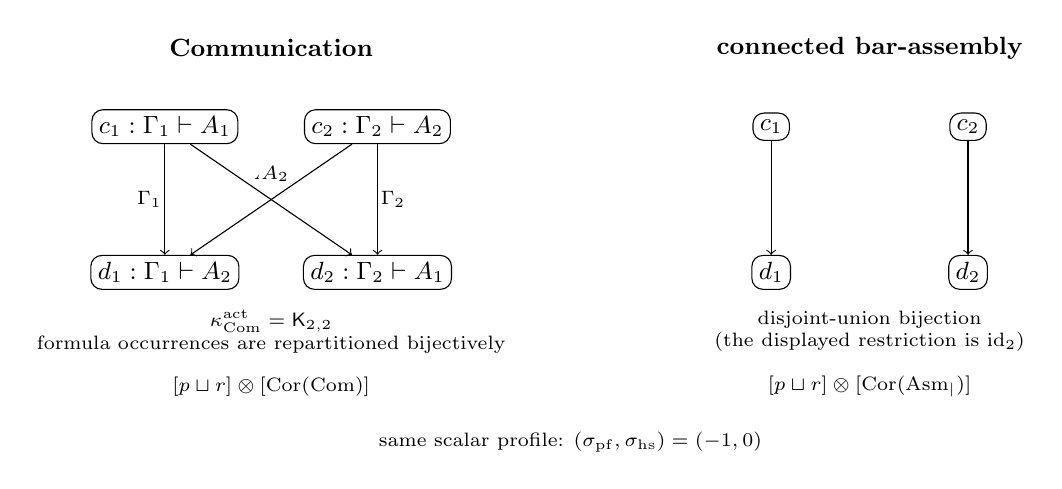
\begin{tikzpicture}[
  every node/.style={font=\small},
  component/.style={draw,rounded corners,inner sep=2.5pt},
  formula/.style={font=\scriptsize,fill=white,inner sep=1pt}
]
  \node[font=\small\bfseries] at (-3.8,2.85) {Communication};
  \node[component] (c1) at (-5.15,1.85) {$c_1:\Gamma_1\ms A_1$};
  \node[component] (c2) at (-2.45,1.85) {$c_2:\Gamma_2\ms A_2$};
  \node[component] (d1) at (-5.15,0) {$d_1:\Gamma_1\ms A_2$};
  \node[component] (d2) at (-2.45,0) {$d_2:\Gamma_2\ms A_1$};
  \draw[->] (c1) -- node[formula,left] {$\Gamma_1$} (d1);
  \draw[->] (c1) -- node[formula,pos=.37,above right] {$A_1$} (d2);
  \draw[->] (c2) -- node[formula,pos=.37,above left] {$A_2$} (d1);
  \draw[->] (c2) -- node[formula,right] {$\Gamma_2$} (d2);
  \node[align=center,font=\scriptsize] at (-3.8,-.75)
    {$\kappa_{\mathrm{Com}}^{\mathrm{act}}=\mathsf K_{2,2}$\\
     formula occurrences are repartitioned bijectively};
  \node[font=\scriptsize] at (-3.8,-1.45)
    {$[p\fjoin r]\otimes[\operatorname{Cor}(\mathrm{Com})]$};

  \node[font=\small\bfseries] at (3.8,2.85)
    {connected bar-assembly};
  \node[component] (a1) at (2.55,1.85) {$c_1$};
  \node[component] (a2) at (5.05,1.85) {$c_2$};
  \node[component] (b1) at (2.55,0) {$d_1$};
  \node[component] (b2) at (5.05,0) {$d_2$};
  \draw[->] (a1) -- (b1);
  \draw[->] (a2) -- (b2);
  \node[align=center,font=\scriptsize] at (3.8,-.75)
    {disjoint-union bijection\\
     (the displayed restriction is $\mathrm{id}_2$)};
  \node[font=\scriptsize] at (3.8,-1.45)
    {$[p\fjoin r]\otimes
      [\operatorname{Cor}(\mathrm{Asm}_{\mid})]$};

  \node[font=\scriptsize] at (0,-2.15)
    {same scalar profile:
     $(\sigma_{\mathrm{pf}},\sigma_{\mathrm{hs}})=(-1,0)$};
\end{tikzpicture}
\caption{Component transport at the immediate-input CK cut.  In the
displayed nondegenerate Communication instance, each input component
contributes disjoint formula occurrences to both outputs, giving
\(\mathsf K_{2,2}\) at component level without copying or erasing any
formula occurrence.  Connected bar-assembly instead transports the two
component occurrences bijectively.}
\label{fig:communication-assembly-transport}
\end{figure}

\begin{proposition}[Scalar collision, relational separation]
\label{prop:communication-footprint}
Communication and connected bar-assembly both have
\[
       (\sigma_{\mathrm{pf}},\sigma_{\mathrm{hs}})=(-1,0).
\]
On the nondegenerate active instance, however,
\(\kappa_{\mathrm{Com}}^{\mathrm{act}}=\mathsf K_{2,2}\), which is neither
functional nor inverse-functional, whereas bar-assembly has a
disjoint-union bijection.  Their full formula-occurrence transports are
bijective.

For compatible complete proofs \(p,r\), cutting at their roots gives
\[
\begin{aligned}
 (\mathrm{id}\otimes\operatorname{pr}_1)\DeltaCK[\mathrm{Com}(p,r)]
   &=[p\fjoin r]\otimes[\operatorname{Cor}(\mathrm{Com})],\\
 (\mathrm{id}\otimes\operatorname{pr}_1)\DeltaCK[\mathrm{Asm}_{\mid}(p,r)]
   &=[p\fjoin r]\otimes[\operatorname{Cor}(\mathrm{Asm}_{\mid})].
\end{aligned}
\eqtag\label{eq:communication-assembly-extraction}
\]
The corresponding immediate-input entries of \(\mathsf{CT}\) therefore
have the same cut addresses and scalar size.  Their restrictions to the
two active input and output components carry, respectively,
\(\mathsf K_{2,2}\) and \(\mathrm{id}_2\); the full relations additionally
carry every passive component occurrence.
\end{proposition}

\begin{proof}
Both occurrences have two proof premises and preserve the total number of
displayed components, giving the scalar pair.  Equations
\eqref{eq:communication-k22} and
\eqref{eq:communication-occurrences} give the two incidence claims.
Bar-assembly sends each premise component to its own output component.
Final-rule extraction and Proposition~\ref{prop:ck-component-profile} give
the displayed CK and component-trace statements.
\end{proof}

\begin{corollary}[Component-transport obstruction to macro-realisation]
\label{cor:communication-macro-obstruction}
Let \(\mathcal S\) be a fragment whose every concrete rule occurrence has
a functional component relation.  Then every proof context generated by
\(\mathcal S\) has functional composite component transport.  Hence no
context in \(\mathcal S\) with the typed interface of a nondegenerate
Communication instance can realise its active
\(\mathsf K_{2,2}\)-transport.  Dually, the same conclusion follows if
all generating relations are inverse-functional.
\end{corollary}

\begin{proof}
Functionality and inverse-functionality are preserved by disjoint union
and relational composition
(Lemma~\ref{thm:structural-footprints}), whereas
\(\mathsf K_{2,2}\) has neither property.
\end{proof}

Thus the component trace is not merely descriptive: it obstructs
macro-realisation of Communication in a fragment whose local
rules are uniformly splitting-free (all local rule traces are functional)
or uniformly merger-free (all local rule traces are inverse-functional).  The uniformity
is essential: Example~\ref{ex:splitting-component-calibration} shows that
mixed splitting and merging traces can compose to \(\mathsf K_{2,2}\) at
the level of bare component transport.  This defeats that bare relational
obstruction only; it does not construct a correctly typed Communication
macro.

\begin{example}[Splitting calibrates the component criterion]
\label{ex:splitting-component-calibration}
Avron's intuitionistic Splitting rule in GLC is
\[
\frac{
 \mathcal G\mid\Gamma,\Delta\ms A\mid\mathcal H
}{
 \mathcal G\mid\Gamma\ms A
 \mid\Delta\ms A\mid\mathcal H
}\;(\mathrm{SI})
\]
\cite[\S III.1.2]{avron1996hypersequents}.  If \(c\) is the active
input component and \(d_\Gamma,d_\Delta\) the two active outputs, then
\[
 \kappa_{\mathrm{SI}}^{\mathrm{act}}
   =\{(c,d_\Gamma),(c,d_\Delta)\},\qquad
 (\sigma_{\mathrm{pf}},\sigma_{\mathrm{hs}})=(0,+1).
\eqtag\label{eq:splitting-component-profile}
\]
Thus Splitting is nonfunctional but inverse-functional on active
components; at formula-occurrence level it also copies the succedent
occurrence \(A\).  It has the same scalar pair as external Weakening
which adds one component, but that rule is functional and has an
unsupported output, hence is nonsurjective.  The relation separates the
two structural actions which the scalar pair identifies.

This also calibrates the limit of
Corollary~\ref{cor:communication-macro-obstruction}.  Communication-free
GLC still contains Splitting and external Contraction.  At the level of
bare component relations, a contraction trace
\(
\{(c_1,e),(c_2,e)\}
\)
followed by the splitting trace
\(
\{(e,d_1),(e,d_2)\}
\)
composes to \(\mathsf K_{2,2}\).  Component transport alone therefore
does not prove the Gentzen-Cut-free nondefinability of Communication in
that fragment; the analytic-support separation below is strictly
stronger.
\end{example}

\paragraph{Why the residue is not the separator here.}
The relative residue from Section~\ref{sec:harmony} compares contexts only
when they share one typed premise telescope and root boundary.  Generic
Communication and bar-assembly do not share such an interface:
bar-assembly retains the two premise hypersequents as disjoint output
blocks, while Communication repartitions their active formula
occurrences.  Even when interfaces do agree, every one-vertex corolla has
zero residue by \eqref{eq:corolla-residue-zero}.
Final-corolla extraction and the CK-resolved component relation are
therefore essential here: they distinguish root-level component transport
which scalar CK cut data and the input-relative residue leave unresolved.

The scalar defects check boundary arithmetic; the component relation
classifies the relevant transport.  The immediate-input cut exposes
two independent hyperproofs together with the two-punctured Communication
corolla whose concrete rule instance crosses their active components.

\subsection{Prelinearity and a resource-sensitive check}

Communication yields the familiar prelinearity derivation
\[
\begin{aligned}
 A\ms A,\ B\ms B
 &\xRightarrow{\ \mathrm{Com}\ }
       A\ms B\mid B\ms A\\
 &\xRightarrow{\ 2(\to R)\ }
       \ms A\to B\mid\ms B\to A\\
 &\xRightarrow{\ 2(\lor R),\,\mathrm{EC}\ }
       \ms (A\to B)\lor(B\to A).
\end{aligned}
\eqtag\label{eq:prelinearity-derivation}
\]
Here \(\mathrm{EC}\) is external Contraction.  The soundness, completeness,
and Gentzen-Cut elimination of Avron's hypersequent calculus GLC for
Dummett's logic LC, and the
connection of Communication with prelinearity, are inherited results
\cite{avron1991,avron1996hypersequents,
baazciabattonifermuller2003}.  The present calculation is
proof-intensional.  Let \(C_{\mathrm{lin}}(-)\) be the outer context
formed by the two \((\to R)\)-steps, the two \((\lor R)\)-steps, and
external Contraction, and put
\[
 t_{\mathrm{lin}}
   =C_{\mathrm{lin}}\bigl(
       \mathrm{Com}(\mathrm{id}_A,\mathrm{id}_B)\bigr).
\]
The CK cut at the two identity roots contributes the explicit tensor
\[
 [\mathrm{id}_A\fjoin\mathrm{id}_B]\ \otimes\
 \boxed{\bigl[
 C_{\mathrm{lin}}\bigl(\mathrm{Com}(\Box_A,\Box_B)\bigr)
 \bigr]}
 \quad\text{to}\quad \DeltaCK[t_{\mathrm{lin}}].
\eqtag\label{eq:prelinearity-ck-factor}
\]
The boxed retained factor carries two premise obligations, the
\(\mathsf K_{2,2}\) Communication relation at its embedded corolla, and
the later component-local logical and contraction steps.  Retrospectively
it records how the two identity proofs were recombined; prospectively it
can accept any proofs of the same two hypersequent premises.

The same active-component relation is not an artefact of internal Weakening or
Contraction.  HUL, the hypersequent calculus for uninorm logic, is based on
multiplicative--additive intuitionistic linear logic and has no general
internal Weakening or Contraction rules.  Its empty-shared-side
Communication instance is
\[
\frac{
 p:\Gamma_1,\Delta_1\ms\Psi_1
 \qquad
 r:\Gamma_2,\Delta_2\ms\Psi_2
}{
 \Gamma_1,\Gamma_2\ms\Psi_1
 \mid
 \Delta_1,\Delta_2\ms\Psi_2
}\;(\mathrm{Com}_{\mathrm{UL}}).
\eqtag\label{eq:hul-communication}
\]
Whenever both premises contribute occurrences to both output components,
its active relation is \(\mathsf K_{2,2}\) and its occurrence relation is
bijective.  In particular, the identity instance
\[
       B\ms B\qquad A\ms A
       \quad\Longrightarrow\quad
       A\ms B\mid B\ms A
\eqtag\label{eq:hul-comparability}
\]
has this profile.  No internal Weakening or Contraction occurrence appears in the
calculation.  We rely on the established metatheory of HUL
\cite{metcalfemontagna2007,baldi2014}.

\subsection{Consequence equivalence versus analytic proof structure}

Communication is consequence-conservative in full GLC but analytically
intensional in its Gentzen-Cut-free fragment.  Let \(C^+\) be GLC and let
\(C^-\) be the system obtained by deleting Communication while retaining
all other GLC rules, in particular conjunction, Splitting, and Gentzen
Cut.
For any equipped calculus \(C\), write \(H_C\) for its proof-tree Hopf
algebra and put
\[
\begin{aligned}
 \operatorname{Conseq}(C)
   &=\{G:\Prf_C(G)\ne\varnothing\},\\
 \operatorname{An}_{D}(C)
   &=\{G:\Prf_C^{\neg D}(G)\ne\varnothing\}\\
   &=\left\{G:
      (H_C/I_D)_{\mathrm{cl}}^{\mathrm{con}}[G]\ne0
     \right\}.
\end{aligned}
\eqtag\label{eq:consequence-analytic-support}
\]
The second set is the support of direct connected complete proofs avoiding
the constructor family \(D\); its quotient presentation uses the sector
notation fixed at the start of Section~\ref{sec:identity}.

\begin{proposition}[Communication as analytic intensional enrichment]
\label{prop:communication-analytic-conservativity}
On GLC hypersequent boundaries,
\[
 \operatorname{Conseq}(C^-)=\operatorname{Conseq}(C^+),
 \qquad
 \operatorname{An}_{\mathrm{GCut}}(C^-)
   \subsetneq
 \operatorname{An}_{\mathrm{GCut}}(C^+).
\eqtag\label{eq:communication-support-separation}
\]
The first equality holds because Avron derives Communication in \(C^-\)
using conjunction, Splitting, and Gentzen Cut; the second says that this
macro-realisation is unavailable analytically.  For distinct atoms
\(p\ne q\), take
\[
                    G_{p,q}=p\ms q\mid q\ms p
\eqtag\label{eq:communication-atomic-witness}
\]
as a witness to strictness.  It has the direct Gentzen-Cut-free proof
\(t_{p,q}=\mathrm{Com}(\mathrm{id}_p,\mathrm{id}_q)\) in \(C^+\), but no
Gentzen-Cut-free proof in \(C^-\).

The direct proof has reduced CK coproduct
\[
\begin{aligned}
 \overline\Delta_{\mathrm{CK}}[t_{p,q}]
  ={}&
 [\mathrm{id}_p]\otimes
   [\mathrm{Com}(\Box_1,\mathrm{id}_q)]\\
 &+[\mathrm{id}_q]\otimes
   [\mathrm{Com}(\mathrm{id}_p,\Box_2)]\\
 &+[\mathrm{id}_p\fjoin\mathrm{id}_q]\otimes
 [\operatorname{Cor}(\mathrm{Com})].
\end{aligned}
\eqtag\label{eq:communication-analytic-cut}
\]
The constructor-deletion quotient of
Theorem~\ref{thm:constructor-deletion} expresses the inherited separator as
\[
\begin{aligned}
 (H_{C^+}/I_{\mathrm{GCut}})_{\mathrm{cl}}^{\mathrm{con}}[G_{p,q}]
   &\ne0,\\
 (H_{C^-}/I_{\mathrm{GCut}})_{\mathrm{cl}}^{\mathrm{con}}[G_{p,q}]
   &=0
\end{aligned}
\eqtag\label{eq:communication-cut-free-quotient-separation}
\]
\end{proposition}

\begin{proof}
The consequence and Gentzen-Cut-free claims are Avron's derivability and
separation results
\cite[\S III.2.1, Theorem~1]{avron1996hypersequents}.
The three coproduct terms are the three nonempty CK cuts of the two
identity leaves.  The quotient reformulation follows because deleting the
Gentzen-Cut constructors kills exactly the proof presentations which use
that rule.
\end{proof}

Thus equality of ordinary consequence support does not imply equality of
the direct analytic proof operations represented in the
constructor-free quotient.
Constructor deletion sends a Gentzen-Cut-containing proof to zero;
Gentzen-Cut elimination constructs a new proof in the surviving carrier.
Avron's Communication elimination requires Gentzen Cut and sufficient
logical structure, while the atomic separator rules out a Gentzen-Cut-free
replacement in the smaller fragment.  Avron supplies that separation; CK
exhibits the direct proof's three punctured factorisations and crossed
final-corolla relation.

\section{Conclusion}

The CK structure has two positive proof-theoretic readings.  First, the
ancestry-forgetting map is a Hopf morphism from typed proof forests to the
poset Hopf algebra of their dependency orders.  Its cut terms are
presentation-causal frontiers; coproduct iterates encode staged premise-first
assemblies---equivalently, reversals of backward-refinement histories---while
convolution powers of \(\zeta\) and \(\omega_1\) count weak layerings and
fully sequential schedules, respectively.  Via the standard
order-polynomial reciprocity theorem, the antipode evaluates signed strict
layerings; it is not a normalisation procedure.  Histories differing only by
the scheduling of independent refinements present the same context.  Thus
the proof-context carrier records no chosen temporal schedule, while the CK
coproduct retains and enumerates the presentation causality on which the
later proof-net obstruction turns.

Second, substitution-uniform hypothetical proof operations are represented by
open proof terms, and CK gives those operations a compositional resource
observation.  The polynomial
\(\mathsf Q_R(\mathbf z)=\prod_i(1+z_i)^{\nu_i(R)}\) is obtained by filling
formal inputs with probes and evaluating the actual coproduct.  Integrally,
its coefficients count probe selections at distinct occurrences, so the
coefficient \(2\) for a duplicated input is not inferred from a contraction
label.  Use vectors compose under
substitution by matrix multiplication, and probe-conservative CK quotients
must preserve them.  More precisely, if
\(M_R(\mathbf u)=\prod_i u_i^{\nu_i(R)}\), then
\(\mathsf Q_R(\mathbf z)=M_R(\mathbf 1+\mathbf z)\); Hasse derivatives of
\(M_R\) at \(\mathbf1\) count unordered CK probe selections, whereas
ordinary iterated derivatives mark ordered pointings.  This is a finite
occurrence-counting bridge to the combinatorics familiar from differential
linear logic, not a differential or Taylor semantics for the present
carrier.  The representation statement is standard free-term
infrastructure; the incidence morphism, convolution counts, resource
polynomial, and comodule obstructions are the specifically Hopf-algebraic
content.

Proof identity is chosen independently of CK factorisation.  Proof classes
always support filling; they support recursive CK decomposition if and
only if equivalent proofs have the same
multiplicities of equivalent detached evidence and equivalent punctured
remainders.  In that case the algebra of proof classes is the universal
connected filtered Hopf quotient realising precisely those equations.  Local
interface symmetries give a nontrivial positive family: they may forget a
local evidence tag or permute genuinely symmetric premise slots while
transporting every CK cut and its multiplicity.  Material-ground tag
irrelevance is the canonical instance.  For the discrete nullary material
presentation its quotient passes from tagged reasons to extensional primitive
support, commutes with persistent base extension, and retains every compound
logical and structural vertex.  The resource polynomial supplies a further
necessary test: any probe-conservative CK-stable identity must preserve the
input-use vector.  Harmony, input preservation, linear use, and CK stability
therefore remain four distinct requirements; the harmonious tensor reduction
passes the first three in the displayed linear instance and still fails the
fourth.

The negative boundary is equally exact.  No proof congruence containing the
standard MLL proof-net permutation or the harmonious principal tensor
reduction can retain the raw CK coproduct: their exposed factors lie in
different proof-interface sectors.  For local conversions, the
protected-input coaction first removes factorisations internal to designated
supplied proofs, and its residue localises the remaining change; the
class-level criterion then proves the global no-go.  Thus the tensor reduction
preserves its input reasons, non-cut boundary incidence, and component action
but not recursive tree factorisation.  \(\mathbin{\mathrm{tonk}}\) fails at
the earlier proof-theoretic stage because no uniformly typed principal reduct
exists.

The construction begins by decomposing a typed and decorated hypersequent
proof tree into detached subproofs and a punctured root context.
Premise-slot types and component incidence make the retained factor an
operation on a typed filling fibre.  Generic-filler separation shows
conversely that one tuple of fresh, distinctly tagged reasons determines the
raw context which uses them.  The typed CK-cut/context-composition bijection
linearises to the Fa\`a di Bruno identity, and its singleton sector pairs
prospective one-slot insertion with retrospective one-address cutting.

Component transport has its own compositional semantics.  The
occurrence-resolved \(\kappa\)-map respects typed context composition,
and the congruence given by equality of \(\kappa\)-values gives exactly the
quotient which forgets
everything except net component movement.  CK-resolved traces refine that
extensional quotient by retaining where the movement occurs.  In
particular, the crossed \(\mathsf K_{2,2}\) trace of Communication both
separates it from bijective bar-assembly and obstructs its macro-realisation
in a uniformly splitting-free or uniformly merger-free fragment.
Splitting calibrates the limit:
Communication-free GLC already has enough relation-level splitting and
merger to compose a \(\mathsf K_{2,2}\) trace, so Avron's analytic
separator is strictly stronger than that local obstruction.  At class
level, \(C^-\) and \(C^+\) have equal ordinary
consequence support but strictly different Gentzen-Cut-free analytic
support.

The standard constructor quotient and its truncated grammar respectively
reject and enumerate constructor-free presentations.  The associated
Birkhoff
factorisation, for the canonical constructor-membership splitting,
collapses to the same deletion projector; it does not normalise a proof.
Typed reducts, a well-founded strategy, and confluence or determinism
remain proof-theoretic data.  A nontrivial rank-sensitive Birkhoff semantics
would additionally require a target Rota--Baxter algebra, a character which
encodes typed redex data, and a theorem decoding its positive factor as a
chosen normal form; cut rank alone supplies none of these.

None of the fixed-calculus causal or resource results assumes monotonicity
of the material support relation in its formula premises.  They use exact
typed boundaries and already licensed proof occurrences, not premise
Weakening.  Persistent base extension may add grounds while retaining the
old ones and therefore acts by injective Hopf maps.  A genuinely defeasible
change which withdraws an old ground is revisory instead: the fixed-fibre
theorems remain valid, but no forward naturality map is claimed.  Constructor
deletion can remove affected presentations, and punctured contexts expose
replacement obligations; no general dynamics of defeat is claimed.

Two limitations of the tree carrier point toward one graph-level problem.
The proof-net obstruction arises because a tree chooses an ancestry between
rules which the net treats as independent; the extended-multicut
Communication case arises because a tree represents reuse by copied
occurrences rather than one shared input.  A proof-DAG or net carrier with
explicit sharing and native subnet decompositions could address both, but it
would require new notions of admissible cut and filling and a new
coassociativity proof.  It is not obtained by a further quotient of the
present tree coproduct.  A tracelet-style route
\cite{behrkock2022} is one concrete candidate:
present proof construction as typed rewrites, quotient histories only by a
proved shift equivalence of independent rewrites, and define decomposition
on the resulting causal traces rather than attempting to descend raw CK
through proof-net equations.  Formula interfaces and hypersequent-component
data would constrain that independence, but cannot decide it by themselves.
The decisive open test is whether such classes admit typed puncturing and
filling and give the two MLL sequentialisations a common native
decomposition.

A second natural step is a first-order
refinement with explicit eigenvariable and witness data and freshness
support, modulo \(\alpha\)-renaming.  Fully instantiated quantifier
occurrences still have nondependent premise telescopes; only a schematic
presentation in which an exposed name or witness parameter determines
later premise requirements would require a genuinely dependent refinement
of the present judgement-indexed CK-cut/context-composition identity.  The
present framework
therefore supplies positive factorisation-stable proof identities while
distinguishing equality of consequences, identity of proof uses, harmony,
and stability of recursive proof decomposition without reducing one to
another.

\clearpage
\section*{Notation index}

Symbols are grouped by their main scope.  Roman capitals such as \(G,H,K\)
denote hypersequent boundaries unless a more specific meaning is displayed;
lower-case letters are local and are redeclared when their role changes.

\begingroup
\footnotesize
\setlength{\tabcolsep}{3pt}
\renewcommand{\arraystretch}{1.05}
\begin{longtable}{@{}L{1.35cm}L{4.15cm}L{9.55cm}@{}}
\toprule
scope & symbol & meaning\\
\midrule
\endfirsthead
\toprule
scope & symbol & meaning\\
\midrule
\endhead
\midrule
\multicolumn{3}{r}{\footnotesize continued on next page}\\
\endfoot
\bottomrule
\endlastfoot
global & \(\Lang,\Base,\Rules\) & formula language, material base, and admitted rule stock\\
global & \(G,H,K\in\HSeq\) & proof-boundary hypersequents; a sequent is a singleton boundary\\
global & \(\Comp(G),\br(G)\) & component occurrences of \(G\), and their number\\
global & \(a:(G_1,\ldots,G_n)\to G,\operatorname{Cor}(a)\) & concrete rule occurrence and its one-vertex corolla; \(n(a)\) is its proof-input arity\\
global & \(\kappa_a\) & local relation from premise-component occurrences to conclusion-component occurrences\\
global & \(t,u\); \(R\) & derivation trees, complete unless stated; a punctured derivation or proof context, respectively\\
global & \(F,\fjoin,\one\) & proof forest, forest juxtaposition, and empty forest\\
\S1 & \(\Box_p,\Punc(R),\Req_R(p)\) & puncture at address \(p\), puncture set, and required boundary\\
\S1 & \(\Tel(R),\Fill(R)\) & ordered premise telescope and complete filling fibre\\
\S1 & \(\Prf(G),\Ctx(\mathbf H;G)\) & complete \(G\)-proofs and contexts with labelled premise family \(\mathbf H\)\\
\S1 & \(\OpenPrf(X),\mathcal O(\mathbf K;G)\) & open proof-term grammar and contexts indexed by requirement word \(\mathbf K\)\\
\S1 & \(\rootseq(t),\BRoot(F),\Root(F)\) & root boundary of a derivation, block-root profile, and flattened forest boundary\\
\S2 & \(p;\ c\in\mathcal A(t)\) & slot address; CK-admissible cut (neither denotes Gentzen Cut)\\
\S2 & \(\mathbf P^c(t),P^c(t),R^c(t)\) & indexed detached subderivations, their forest product, and punctured remainder\\
\S2 & \(\mathbb W_c(t)\) & address-indexed CK-cut witness retaining the matching of factors and holes\\
\S2 & \([F],\HCK=\Hlic,\DeltaCK,\epsCK\) & basis vector, the proof-tree Hopf algebra with structural or calculus-relative emphasis, CK coproduct, and empty-forest counit\\
\S2 & \(\overline\Delta_{\mathrm{CK}},D_F,\mathfrak G^G_{\mathbf K}\) & proper-cut coproduct, premise-ancestry poset, and context Green series\\
\S2 & \(\mathsf{Cut}_t(q),\Delta_{\mathrm{CK}}^{(1)},\triangleright\) & cut-size polynomial, singleton-cut coproduct, and one-slot insertion product\\
\S2 & \(\mathsf{Hist}_C,\operatorname{Anc},H^{\mathbb Z}_{\mathsf{ForPos}}\) & backward-refinement histories, ancestry-forgetting Hopf map, and poset Hopf algebra of rooted forests\\
\S2 & \(\zeta,\omega_1\) & all-ones character and degree-one infinitesimal character; their convolution powers count causal layers and schedules\\
\S2--5 & \(I_D,q_D\) & constructor-deletion ideal and quotient; deletion rejects rather than reduces\\
\S3 & \(C_G^{\mathrm{con}},\delta_G\) & connected \(G\)-rooted derivation space and its root-preserving coaction\\
\S3 & \(\sigma_{\mathrm{pf}},\sigma_{\mathrm{hs}},\kappa_R,\mathsf{CT}(t)\) & scalar defects, composite component transport, and CK-resolved transport profile\\
\S3 & \(E,\sim_E,I_E,q_E,A_E\) & proof congruence, its ideal, quotient map, and algebra of proof classes\\
\S3 & \(\mathsf{Int}(F),\mathcal S,E_{\mathcal S}\) & open proof-interface signature, local interface symmetries, and their generated proof congruence\\
\S3 & \(E_{\mathrm{gr}},\Base_{\mathrm{ext}}\) & material-ground tag irrelevance and the extensionalised nullary material base\\
\S3 & \(N_F^E(U,V)\) & multiplicity of proper CK factorisations into \(E\)-classes \(U,V\)\\
\S4 & \(\Xi=(x_i:G_i),V_\Xi,\lambda_\Xi\) & labelled input telescope, pointed input space, and input coaction\\
\S4 & \(\mathsf{Sub}_C,T_C(X)_G,\alpha_R,\nu_i(R)\) & proof-substitution category, open proof terms, independent-copy alias map, and input-use number\\
\S4 & \(\varphi_{\mathbf z},\mathsf Q_R(\mathbf z)\) & probe character and CK resource polynomial\\
\S4 & \(M_R(\mathbf u),\operatorname{Pt}_{\mathbf r}(R),D^{[\mathbf r]}\) & use monomial, ordered pointings, and multivariate Hasse derivative\\
\S4 & \(e_s,\Omega_s,\operatorname{Res}_{s,s'},\operatorname{Res}^{\mathsf{Prot}}_{e_0,e_1}\) & context evaluation, context-relative residue, full-input replacement residue, and protected replacement residue\\
\S4 & \(\mathsf{Prot},\chi,J\) & protected input positions, comparison difference, and generated comparison ideal\\
\S4 & \(I_{\mathrm{bg}},q_{\mathrm{bg}},K_A\) & accepted background ideal, its quotient map, and Gentzen-Cut corolla\\
\S4 & \(\Pi_{\mathrm{cf}},\Pi_{\mathrm{bad}},\star,S_{\mathrm{CK}}\) & constructor-free/bad projectors, convolution, and antipode\\
\S5 & \(\mathrm{Com},\mathrm{Asm}_{\mid},\mathrm{SI}\) & Communication, connected bar-assembly, and Splitting vertices\\
\S5 & \(\operatorname{Conseq}(C),\operatorname{An}_D(C)\) & ordinary consequence support and direct \(D\)-free analytic support\\
\end{longtable}
\endgroup

Two conventions are especially important.  A proof forest is a multiset of
proof-labelled derivation trees, not an ordinary displayed hypersequent.
A CK cut decomposes an existing tree; Gentzen Cut is a rule occurrence;
filling or context composition inserts a derivation at a typed puncture.
Finally, \([F]\) is a linear basis vector, whereas \([F]_E\) is an
\(E\)-equivalence class.

Several familiar glyphs are deliberately local.  The \(\Delta\) in a
sequent such as \(\Gamma\ms\Delta\) is a formula multiset, unlike
\(\DeltaCK\).  The proof polynomial \(P_{\Base,\Rules}\) is unrelated to
the detached factor \(P^c(t)\).  The letter \(C\) may denote a displayed
proof context or, when declared as \(C=(\Base,\Rules)\), an equipped
calculus.  Finally, \(D_F\) is a premise-ancestry poset, whereas \(D\) in
\(I_D\) and \(\operatorname{An}_D\) is a family of constructor tags.

\begin{thebibliography}{99}
\footnotesize
\raggedright
\setlength{\itemsep}{0pt}
\setlength{\parskip}{0pt}

\bibitem{abbott2003derivatives}
M.~Abbott, T.~Altenkirch, N.~Ghani, and C.~McBride.
\newblock Derivatives of containers.
\newblock In \emph{Typed Lambda Calculi and Applications}, volume 2701 of
\emph{Lecture Notes in Computer Science}, pages 16--30. Springer, 2003.
\newblock doi:10.1007/3-540-44904-3\_2.

\bibitem{aguiarbergeronsottile2006}
M.~Aguiar, N.~Bergeron, and F.~Sottile.
\newblock Combinatorial Hopf algebras and generalized
Dehn--Sommerville relations.
\newblock \emph{Compositio Mathematica}, 142(1):1--30, 2006.
\newblock doi:10.1112/S0010437X0500165X.

\bibitem{andreoli1992}
J.-M.~Andreoli.
\newblock Logic programming with focusing proofs in linear logic.
\newblock \emph{Journal of Logic and Computation}, 2(3):297--347, 1992.
\newblock doi:10.1093/logcom/2.3.297.

\bibitem{avron1991}
A.~Avron.
\newblock Hypersequents, logical consequence and intermediate logics for
concurrency.
\newblock \emph{Annals of Mathematics and Artificial Intelligence},
4:225--248, 1991.

\bibitem{avron1996hypersequents}
A.~Avron.
\newblock The method of hypersequents in the proof theory of propositional
non-classical logics.
\newblock In W.~Hodges, M.~Hyland, C.~Steinhorn, and J.~Truss, editors,
\emph{Logic: From Foundations to Applications}, pages 1--32.
Oxford University Press, 1996.

\bibitem{baazciabattonifermuller2003}
M.~Baaz, A.~Ciabattoni, and C.~G. Ferm\"uller.
\newblock Hypersequent calculi for G\"odel logics---a survey.
\newblock \emph{Journal of Logic and Computation}, 13(6):835--861, 2003.
\newblock doi:10.1093/logcom/13.6.835.

\bibitem{baldi2014}
P.~Baldi.
\newblock A note on standard completeness for some axiomatic extensions of
uninorm logic.
\newblock \emph{Soft Computing}, 18:1463--1470, 2014.
\newblock doi:10.1007/s00500-014-1265-1.

\bibitem{barrosonascimentopiotrovskapimentel2026}
V.~Barroso-Nascimento, E.~Piotrovskaya, and E.~Pimentel.
\newblock A sequent calculus perspective on base-extension semantics.
\newblock In \emph{Automated Reasoning with Analytic Tableaux and Related
Methods}, volume 15980 of \emph{Lecture Notes in Artificial Intelligence},
pages 3--21. Springer, 2026.
\newblock doi:10.1007/978-3-032-06085-3\_1.

\bibitem{behrkock2022}
N.~Behr and J.~Kock.
\newblock Tracelet Hopf algebras and decomposition spaces (extended
abstract).
\newblock \emph{Electronic Proceedings in Theoretical Computer Science},
372:323--337, 2022.
\newblock doi:10.4204/EPTCS.372.23.

\bibitem{benson1989}
D.~B. Benson.
\newblock Bialgebras: Some foundations for distributed and concurrent
computation.
\newblock \emph{Fundamenta Informaticae}, 12(4):427--486, 1989.
\newblock doi:10.3233/FI-1989-12402.

\bibitem{blutescott1998}
R.~F. Blute and P.~J. Scott.
\newblock The shuffle Hopf algebra and noncommutative full completeness.
\newblock \emph{Journal of Symbolic Logic}, 63(4):1413--1436, 1998.
\newblock doi:10.2307/2586659.

\bibitem{calaqueebrahimifardmanchon2011}
D.~Calaque, K.~Ebrahimi-Fard, and D.~Manchon.
\newblock Two interacting Hopf algebras of trees: A Hopf-algebraic approach
to composition and substitution of B-series.
\newblock \emph{Advances in Applied Mathematics}, 47(2):282--308, 2011.
\newblock doi:10.1016/j.aam.2009.08.003.

\bibitem{chapoton2002}
F.~Chapoton.
\newblock Rooted trees and an exponential-like series.
\newblock Preprint, 2002.
\newblock arXiv:math/0209104.

\bibitem{chapotonlivernet2001}
F.~Chapoton and M.~Livernet.
\newblock Pre-Lie algebras and the rooted trees operad.
\newblock \emph{International Mathematics Research Notices},
2001(8):395--408, 2001.

\bibitem{castellanyoshida2019}
S.~Castellan and N.~Yoshida.
\newblock Causality in linear logic: Full completeness and injectivity
(unit-free multiplicative-additive fragment).
\newblock In \emph{Foundations of Software Science and Computation
Structures}, volume 11425 of \emph{Lecture Notes in Computer Science},
pages 150--168. Springer, 2019.
\newblock doi:10.1007/978-3-030-17127-8\_9.

\bibitem{chaudhurimillersaurin2008}
K.~Chaudhuri, D.~Miller, and A.~Saurin.
\newblock Canonical sequent proofs via multi-focusing.
\newblock In G.~Ausiello, J.~Karhum\"aki, G.~Mauri, and L.~Ong, editors,
\emph{Fifth IFIP International Conference on Theoretical Computer Science},
volume 273 of \emph{IFIP Advances in Information and Communication
Technology}, pages 383--396. Springer, 2008.
\newblock doi:10.1007/978-0-387-09680-3\_26.

\bibitem{conneskreimer1998}
A.~Connes and D.~Kreimer.
\newblock Hopf algebras, renormalization and noncommutative geometry.
\newblock \emph{Communications in Mathematical Physics}, 199(1):203--242,
1998.

\bibitem{dummett1991}
M.~Dummett.
\newblock \emph{The Logical Basis of Metaphysics}.
\newblock Harvard University Press, Cambridge, MA, 1991.

\bibitem{ebrahimifardguokreimer2004}
K.~Ebrahimi-Fard, L.~Guo, and D.~Kreimer.
\newblock Spitzer's identity and the algebraic Birkhoff decomposition in
perturbative quantum field theory.
\newblock \emph{Journal of Physics A: Mathematical and General},
37(45):11037--11052, 2004.
\newblock doi:10.1088/0305-4470/37/45/020.

\bibitem{ehrenborg1996}
R.~Ehrenborg.
\newblock On posets and Hopf algebras.
\newblock \emph{Advances in Mathematics}, 119(1):1--25, 1996.
\newblock doi:10.1006/aima.1996.0026.

\bibitem{ehrhard2018dll}
T.~Ehrhard.
\newblock An introduction to differential linear logic: proof-nets, models
and antiderivatives.
\newblock \emph{Mathematical Structures in Computer Science},
28(7):995--1060, 2018.
\newblock doi:10.1017/S0960129516000372.

\bibitem{ehrhardregnier2003}
T.~Ehrhard and L.~Regnier.
\newblock The differential lambda-calculus.
\newblock \emph{Theoretical Computer Science}, 309(1--3):1--41, 2003.
\newblock doi:10.1016/S0304-3975(03)00392-X.

\bibitem{ehrhardregnier2006}
T.~Ehrhard and L.~Regnier.
\newblock Differential interaction nets.
\newblock \emph{Theoretical Computer Science}, 364(2):166--195, 2006.
\newblock doi:10.1016/j.tcs.2006.08.003.

\bibitem{ehrhardregnier2008}
T.~Ehrhard and L.~Regnier.
\newblock Uniformity and the Taylor expansion of ordinary lambda-terms.
\newblock \emph{Theoretical Computer Science}, 403(2--3):347--372, 2008.
\newblock doi:10.1016/j.tcs.2008.06.001.

\bibitem{foissy2002}
L.~Foissy.
\newblock Les alg\`ebres de Hopf des arbres enracin\'es d\'ecor\'es, I.
\newblock \emph{Bulletin des Sciences Math\'ematiques}, 126(3):193--239,
2002.

\bibitem{foissy2021typed}
L.~Foissy.
\newblock Algebraic structures on typed decorated rooted trees.
\newblock \emph{SIGMA}, 17:086, 2021.
\newblock doi:10.3842/SIGMA.2021.086.

\bibitem{frabettimanchon2015}
A.~Frabetti and D.~Manchon.
\newblock Five interpretations of Fa\`a di Bruno's formula.
\newblock In K.~Ebrahimi-Fard and F.~Fauvet, editors,
\emph{Fa\`a di Bruno Hopf Algebras, Dyson--Schwinger Equations, and
Lie--Butcher Series}, pages 91--147. European Mathematical Society, 2015.
\newblock doi:10.4171/143-1/3.

\bibitem{galvezkocktonks2014}
I.~G\'alvez-Carrillo, J.~Kock, and A.~Tonks.
\newblock Groupoids and Fa\`a di Bruno formulae for Green functions in
bialgebras of trees.
\newblock \emph{Advances in Mathematics}, 254:79--117, 2014.
\newblock doi:10.1016/j.aim.2013.12.015.

\bibitem{girard1987}
J.-Y.~Girard.
\newblock Linear logic.
\newblock \emph{Theoretical Computer Science}, 50(1):1--101, 1987.
\newblock doi:10.1016/0304-3975(87)90045-4.

\bibitem{gheorghiuGuPymIMLL}
A.~V. Gheorghiu, T.~Gu, and D.~J. Pym.
\newblock Proof-theoretic semantics for intuitionistic multiplicative
linear logic.
\newblock \emph{Studia Logica}, 114(2):451--511, 2026.
\newblock doi:10.1007/s11225-024-10158-6.

\bibitem{guGheorghiuPymBI}
T.~Gu, A.~V. Gheorghiu, and D.~J. Pym.
\newblock Proof-theoretic semantics for the logic of bunched implications.
\newblock \emph{Studia Logica}, 2025.
\newblock doi:10.1007/s11225-025-10202-z.

\bibitem{kock2017}
J.~Kock.
\newblock Polynomial functors and combinatorial Dyson--Schwinger equations.
\newblock \emph{Journal of Mathematical Physics}, 58:041703, 2017.
\newblock doi:10.1063/1.4977012.

\bibitem{kockweber2019}
J.~Kock and M.~Weber.
\newblock Fa\`a di Bruno for operads and internal algebras.
\newblock \emph{Journal of the London Mathematical Society},
99:919--944, 2019.
\newblock doi:10.1112/jlms.12201.

\bibitem{mcbride2001}
C.~McBride.
\newblock The derivative of a regular type is its type of one-hole contexts.
\newblock Unpublished extended abstract, 2001.
\newblock \url{https://strictlypositive.org/diff.pdf}.

\bibitem{metcalfemontagna2007}
G.~Metcalfe and F.~Montagna.
\newblock Substructural fuzzy logics.
\newblock \emph{Journal of Symbolic Logic}, 72(3):834--864, 2007.
\newblock doi:10.2178/jsl/1191333844.

\bibitem{nielsenplotkinwinskel1981}
M.~Nielsen, G.~Plotkin, and G.~Winskel.
\newblock Petri nets, event structures and domains, part I.
\newblock \emph{Theoretical Computer Science}, 13(1):85--108, 1981.
\newblock doi:10.1016/0304-3975(81)90112-2.

\bibitem{pistonetranchini2024}
P.~Pistone and L.~Tranchini.
\newblock Intensional harmony as isomorphism.
\newblock In T.~Piecha and K.~F. Wehmeier, editors,
\emph{Peter Schroeder-Heister on Proof-Theoretic Semantics},
volume 29 of \emph{Outstanding Contributions to Logic},
pages 315--337. Springer, Cham, 2024.

\bibitem{prior1960}
A.~N. Prior.
\newblock The runabout inference-ticket.
\newblock \emph{Analysis}, 21(2):38--39, 1960.
\newblock doi:10.1093/analys/21.2.38.

\bibitem{prawitz1965}
D.~Prawitz.
\newblock \emph{Natural Deduction: A Proof-Theoretical Study}.
\newblock Stockholm Studies in Philosophy 3. Almqvist \& Wiksell,
Stockholm, 1965.

\bibitem{sandqvist2015}
T.~Sandqvist.
\newblock Base-extension semantics for intuitionistic sentential logic.
\newblock \emph{Logic Journal of the IGPL}, 23(5):719--731, 2015.
\newblock doi:10.1093/jigpal/jzv021.

\bibitem{schroederheister2015}
P.~Schroeder-Heister.
\newblock Harmony in proof-theoretic semantics: A reductive analysis.
\newblock In H.~Wansing, editor, \emph{Dag Prawitz on Proofs and Meaning},
Outstanding Contributions to Logic 7, pages 329--358.
Springer, Cham, 2015.

\bibitem{stanley1972}
R.~P. Stanley.
\newblock \emph{Ordered Structures and Partitions}.
\newblock Memoirs of the American Mathematical Society 119.
American Mathematical Society, Providence, RI, 1972.

\end{thebibliography}

\end{document}
